\documentclass[a4paper,12pt]{ctexart}

\usepackage{geometry}
\usepackage{amsmath}
\usepackage{amssymb}
\usepackage{xcolor}

% Force graphicx to use final mode and display real figures
\usepackage[final]{graphicx}
\setkeys{Gin}{draft=false}

% Figure directory
\graphicspath{{pic/}{./pic/}}

% Accepted graphics extensions
\DeclareGraphicsExtensions{.png,.jpg,.jpeg,.pdf}

\usepackage{multirow}
\usepackage{fancyhdr}
\usepackage{float}
\usepackage{subcaption}
\usepackage{booktabs}
\usepackage{tabularx}
\usepackage{array}
\usepackage{longtable}
\usepackage{bm}
\usepackage[hidelinks]{hyperref}
\usepackage[numbers,sort&compress]{natbib}

\geometry{left=2.5cm, right=2.5cm, top=2.5cm, bottom=2.5cm}

\renewcommand{\figurename}{Figure}
\renewcommand{\abstractname}{Abstract}
\numberwithin{equation}{section}
\renewcommand{\theequation}{\thesection.\arabic{equation}}

\pagestyle{fancy}
\fancyhf{}
\fancyfoot[C]{\thepage}

\newcommand{\vb}[1]{\bm{#1}}
\newcommand{\vx}{\vb{x}}
\newcommand{\vn}{\vb{n}}
\newcommand{\vs}{\vb{s}}
\newcommand{\vq}{\vb{q}}
\newcommand{\vc}{\vb{c}}
\newcommand{\vxi}{\bm{\xi}}
\newcommand{\dd}{\mathrm{d}}
\newcommand{\figwidth}{0.32\textwidth}
\newcommand{\TODO}[1]{\textcolor{red}{TODO: #1}}
\newcounter{procedure}
\renewcommand{\theprocedure}{\arabic{procedure}}

\makeatletter
\renewcommand\maketitle{
\begin{center}
\vspace*{1cm}
\LARGE\bfseries \@title
\par\vskip 0.5em
\large \@author
\par\vskip 0.8cm
\end{center}
}
\makeatother

\begin{document}

\title{A coupled DUGKS for transient conduction–radiation in participating media}

\begin{abstract}
Transient heat transfer in participating media couples local thermal diffusion with nonlocal angular radiation. A numerical difficulty is that the energy equation and radiative transfer equation are often advanced by different discretisations, although the radiative source depends on the local temperature and incident radiation at every time step. Here, a coupled discrete unified gas-kinetic scheme (DUGKS) is formulated for gray, absorbing, emitting, and isotropically scattering media. A temperature distribution function represents the energy equation, and a pseudo-time kinetic relaxation equation resolves the radiative intensity. The two fields are advanced on the same control-volume grid, and both interface fluxes are reconstructed from characteristic solutions. This coupling evaluates the radiative source directly at temperature nodes and avoids interpolation between thermal and radiative meshes. The scheme is assessed using one-dimensional slab, two-dimensional square-enclosure, and three-dimensional cubical-enclosure benchmarks. The slab and square-enclosure calculations reproduce reference temperature and heat-flux data, with maximum differences of $1.8\times10^{-3}$ and $4.0\times10^{-3}$ from the corresponding LBM--FVM references. The cubical calculations extend the same update to the Sun et al. benchmark matrix, including scattering, conduction--radiation strength, wall emissivity, and optical thickness. Across these cases, the results show faster heating under stronger radiative exchange and slower heating when scattering reduces absorption or wall emissivity is lowered. The coupled DUGKS therefore provides a single finite-volume kinetic route for transient conduction--radiation simulations from planar to fully three-dimensional participating media, within the gray and isotropic-scattering assumptions tested here.
\end{abstract}

\section{Introduction}
\label{sec:introduction}

Heat transfer in high-temperature participating media depends on the interaction between thermal diffusion and radiative transport. This interaction governs thermal protection systems, combustion chambers, insulation layers, and radiatively active enclosures. Numerical prediction is difficult because the energy equation contains a radiative source, whereas the radiative transfer equation (RTE) contains emission proportional to $T^4$. The resulting coupling is nonlinear, nonlocal, and sensitive to optical thickness, scattering albedo, the conduction--radiation parameter, and geometry. One-dimensional slabs provide a standard benchmark for transient conduction--radiation coupling~\cite{Talukdar2001}. Transient finite-element analyses further illustrate the numerical demands of coupled radiative heat transfer~\cite{Feng2021}. Extensions to anisotropically scattering cylinders and high-temperature media show the additional influence of geometry and coupling strategy~\cite{YasongSun2021,Zhu2024}.

Numerical studies have therefore relied widely on hybrid treatments of the energy equation and the RTE. Early work combined LBM heat conduction with the discrete transfer method~\cite{MishraLankadasu2005} or with an FVM radiation solver~\cite{MishraRoy2007}. Other formulations coupled LBM with the discrete ordinates method~\cite{MondalMishra2007} or adopted a shared-grid LBM--FVM treatment for planar and square media~\cite{Sun2016}. The same benchmark family includes short-time slab solutions~\cite{Sutton1986}, transient scattering calculations~\cite{LinTsai1990}, and two-dimensional rectangular or square enclosures~\cite{YuenTakara1988,WuOu1994}. Sun et al.~\cite{SunMaLi2012} further considered a three-dimensional cubical enclosure using a Chebyshev collocation spectral method, providing a useful transient test matrix for scattering albedo, conduction--radiation parameter, wall emissivity, and optical thickness. This route was subsequently extended to irregular geometries and composite or graded materials~\cite{Abaszadeh2022,Tong2022}. Related models treated graded-index media~\cite{Wei2023} and curved radiative boundaries~\cite{Sharifi2023}. Unstructured radiation models and complex-geometry LBM--FVM algorithms broadened the available spatial discretisations~\cite{Liu2024,Miao2025}. These methods offer accuracy and geometric flexibility. However, they generally advance thermal diffusion and radiative transport through distinct numerical mechanisms.

The discrete unified gas-kinetic scheme (DUGKS) offers a route to reduce this separation. The original DUGKS reconstructs finite-volume interface fluxes from characteristic solutions of the governing kinetic equation~\cite{Guo2013}. Wang et al. subsequently coupled separate velocity and temperature distributions for Boussinesq flows~\cite{Wang2015}. Characteristic reconstruction incorporates transport and relaxation into flux evaluation, while the time step follows a CFL condition rather than fixed lattice streaming. The finite-volume kinetic framework was later extended to conjugate heat transfer~\cite{Tao2021} and immersed-boundary fluid-solid thermal coupling~\cite{Tao2022}. Further developments addressed non-Oberbeck--Boussinesq convection~\cite{Wen2025} and complex thermal flows on hierarchical Cartesian grids~\cite{Tao2025}.

Gas-kinetic schemes have also advanced radiative-transfer modelling. Unified gas-kinetic schemes were first developed for gray RTEs~\cite{SunJiangXu2015} and then extended to frequency-dependent transport~\cite{Sun2015Frequency}. Multidimensional formulations supported unstructured radiation meshes~\cite{Sun2017}, while DUGKS enabled multiscale radiative heat-transfer calculations~\cite{Luo2018}. Later work introduced positive asymptotic-preserving moment treatments~\cite{Xu2021} and accelerated steady DUGKS iterations~\cite{Song2022}. Diffusion synthetic acceleration improved steady radiative calculations~\cite{Song2023}, whereas spatially second-order schemes strengthened accuracy and asymptotic preservation~\cite{Xu2023}. Positive formulations were subsequently extended to nonlinear radiative transfer~\cite{Xu2024,Song2025}. Cylindrical-coordinate systems~\cite{Wang2025Cyl} and three-temperature radiation models~\cite{Li2025} further broadened their scope. Positivity-preserving gray RTE schemes continue to refine kinetic flux construction~\cite{Wang2026}. Collectively, these studies establish gas-kinetic schemes as credible RTE solvers. However, a common DUGKS treatment of thermal and radiative updates in transient benchmarks remains underexplored.

These studies leave a specific numerical question: whether transient conduction and radiative transfer can be advanced within one DUGKS update structure while retaining a direct source coupling on a shared grid. The present study addresses this question for gray participating media. A temperature distribution function represents the energy equation, and a pseudo-time kinetic relaxation equation advances the radiative intensity. Both fields are solved on the same control-volume grid, and both fluxes are obtained through characteristic reconstruction. The radiative source is therefore evaluated at the temperature nodes without inter-mesh interpolation. The formulation is first verified by recomputing representative slab and square-enclosure cases selected from the above literature. It is then applied to the three-dimensional cubical configuration of Sun et al.~\cite{SunMaLi2012}. This ordering keeps the evidence progressive: the one-dimensional case checks the coupled source term, the two-dimensional case checks multidirectional wall exchange and angular sensitivity, and the three-dimensional case tests the same update structure under fully three-component transport, six wall boundaries, and optical-thickness scaling.

\section{Coupled DUGKS formulation for conduction--radiation heat transfer}
\label{sec:coupled_dugks}

This section separates the physical model from its DUGKS discretisation. The continuous model defines the conduction--radiation coupling and nondimensional parameters. The discrete formulation then introduces the temperature and radiation distribution functions, characteristic flux reconstruction, boundary treatment, and time-marching sequence.

\subsection{Gas-kinetic model for transient conduction--radiation problems}
\label{subsec:kinetic_model}

The participating medium is gray, absorbing, emitting, and isotropically scattering. The density $\rho$, specific heat $c_p$, thermal conductivity $k$, absorption coefficient $\kappa_a$, and scattering coefficient $\kappa_s$ are constant. Because the benchmark configurations exclude fluid motion, the macroscopic model contains only the transient energy equation and the RTE. The dimensional energy equation is
\begin{equation*}
\rho c_p\frac{\partial T}{\partial t}=k\nabla^2T-\nabla\cdot\vq_r,
\end{equation*}
where $T$ denotes temperature and $\vq_r$ denotes radiative heat flux. For a gray medium with isotropic scattering, the radiative-flux divergence is
\begin{equation*}
\nabla\cdot\vq_r=\beta(1-\omega)\left(4\sigma T^4-G_d\right),
\end{equation*}
where $\beta=\kappa_a+\kappa_s$ is the extinction coefficient, $\omega=\kappa_s/\beta$ is the scattering albedo, and $\sigma$ is the Stefan--Boltzmann constant. The quantity $G_d$ is the dimensional incident radiation. The RTE along direction $\vs$ is
\begin{equation*}
\vs\cdot\nabla I=-\beta I+\kappa_a I_b+\frac{\kappa_s}{4\pi}\int_{4\pi}I(\vs')\dd\Omega',
\end{equation*}
where $I=I(\vx,\vs)$ is the directional radiation intensity and $I_b=\sigma T^4/\pi$ is the blackbody intensity.

The characteristic length is $L$, and the hot-wall temperature $T_w$ defines the reference temperature. Using the thermal diffusivity $\alpha=k/(\rho c_p)$, the dimensionless variables are
\begin{equation*}
\begin{aligned}
\theta&=\frac{T}{T_w},\\
\vx^*&=\frac{\vx}{L},\\
\zeta&=\frac{\alpha t}{L^2},\\
G&=\frac{G_d}{4\sigma T_w^4}.
\end{aligned}
\end{equation*}
The optical thickness is $\tau_L=\beta L$, and the conduction--radiation parameter is
\begin{equation*}
N=\frac{\kappa_a k}{4\sigma T_w^3}.
\end{equation*}
The dimensionless energy equation is
\begin{equation}
\begin{aligned}
\frac{\partial\theta}{\partial\zeta}&=\nabla^2\theta+Q_r,
\\
Q_r&=\frac{1-\omega}{N}\left(G-\theta^4\right),
\end{aligned}
\label{eq:dimensionless_energy}
\end{equation}
where $Q_r$ is the dimensionless radiative source. Small $N$ indicates strong radiative exchange relative to conduction, whereas large $N$ corresponds to a conduction-dominated regime.

To represent Eq.~\eqref{eq:dimensionless_energy} within DUGKS, a temperature distribution function $g=g(\vx,\vxi,t)$ is introduced. With zero macroscopic velocity, its kinetic equation is
\begin{equation}
\begin{aligned}
\frac{\partial g}{\partial t}+\vxi\cdot\nabla g&=\Omega^g+S^g,
\\
\Omega^g&=\frac{g^{eq}-g}{\tau_g},
\end{aligned}
\label{eq:thermal_kinetic_continuous}
\end{equation}
where $\tau_g$ is the thermal relaxation time. The equilibrium and radiative-source distributions are
\begin{equation*}
\begin{aligned}
g^{eq}&=\theta\,\mathcal{M}(\vxi),
\\
S^g&=Q_r\,\mathcal{M}(\vxi),
\end{aligned}
\end{equation*}
where $\mathcal{M}$ is a normalised weight function. The zeroth moment of Eq.~\eqref{eq:thermal_kinetic_continuous} recovers the energy equation because $\int\Omega^g\dd\vxi=0$ and $\int S^g\dd\vxi=Q_r$.

The steady RTE is solved through a pseudo-time kinetic relaxation equation. For each angular control volume, indexed by $m$, the dimensionless intensity $I_m$ satisfies
\begin{equation}
\begin{aligned}
\frac{\partial I_m}{\partial \chi}+\vs_m\cdot\nabla I_m&=\Omega_m^I,
\\
\Omega_m^I&=\frac{I_m^{eq}-I_m}{\tau_I},
\end{aligned}
\label{eq:radiation_kinetic}
\end{equation}
where $\chi$ is pseudo time and $\tau_I$ is the radiative relaxation time. The present calculations use $\tau_I=1$. The equilibrium intensity is
\begin{equation}
I_m^{eq}=(1-\omega)\theta^4+\omega G.
\label{eq:radiation_equilibrium}
\end{equation}
Angular moments of the intensity give the incident radiation and radiative heat flux,
\begin{equation}
\begin{aligned}
G&=\sum_{m=1}^{M}w_m I_m,
\\
\vq_r&=\sum_{m=1}^{M}w_m\vs_m I_m,
\end{aligned}
\label{eq:angular_moments}
\end{equation}
where $w_m$ is the angular quadrature weight. For the one-dimensional slab, the zenith interval $[0,\pi]$ is divided into $M=16$ angular control volumes. Over an interval $[\theta_l,\theta_r]$, the quadrature weight and representative direction cosine are
\begin{equation*}
\begin{aligned}
w_m&=\frac{1}{2}(\cos\theta_l-\cos\theta_r),
\\
\mu_m&=\frac{1}{2}(\cos\theta_l+\cos\theta_r).
\end{aligned}
\end{equation*}
The corresponding directional heat-flux weight is
\begin{equation*}
w_m^q=\frac{1}{4}(\sin^2\theta_r-\sin^2\theta_l).
\end{equation*}
For the two-dimensional square enclosure, polar and azimuthal control volumes discretise the solid angle. The angular data contain the projected directions $(\mu_{x,m},\mu_{y,m})$, solid-angle weights $w_m$, and heat-flux weights used along the centreline. The fully three-dimensional cubical case uses the same angular finite-volume idea but retains all three components of the representative direction vector, as detailed in Sec.~\ref{subsec:three_dimensional_extension}. A CFL condition based on the largest projected transport speed determines the pseudo-time step. Equations~\eqref{eq:thermal_kinetic_continuous} and \eqref{eq:radiation_kinetic} form the coupled kinetic model. The radiation equation depends on local emission $\theta^4$, whereas the temperature equation depends on the incident radiation $G$ through $Q_r$. The numerical coupling therefore occurs through the source and equilibrium terms rather than through a separate mesh-transfer step.

\subsection{DUGKS for the temperature field}
\label{subsec:temperature_dugks}

The computational domain is divided into finite-volume cells $V_j$ centred at $\vx_j$. After discretisation of velocity space by $\vxi_i$, the temperature kinetic equation becomes
\begin{equation}
\begin{aligned}
\frac{\partial g_i}{\partial t}+\vxi_i\cdot\nabla g_i&=\Omega_i^g+S_i^g,
\\
\Omega_i^g&=\frac{g_i^{eq}-g_i}{\tau_g},
\\
S_i^g&=w_i Q_r,
\end{aligned}
\label{eq:thermal_kinetic_discrete}
\end{equation}
where $w_i$ is the velocity quadrature weight. Without macroscopic motion, the equilibrium distribution is
\begin{equation*}
g_i^{eq}=w_i\theta.
\end{equation*}
Equation~\eqref{eq:thermal_kinetic_discrete} is integrated over $V_j$ from $t_n$ to $t_{n+1}$. Applying midpoint integration to the flux and trapezoidal integration to the collision and source terms gives
\begin{equation}
\tilde g_{i,j}^{n+1}=\tilde g_{i,j}^{+,n}-\frac{\Delta t}{|V_j|}F_{i,j}^{n+1/2},
\label{eq:g_update}
\end{equation}
where
\begin{equation}
\begin{aligned}
F_{i,j}^{n+1/2}&=\int_{\partial V_j}(\vxi_i\cdot\vn)g_i(\vx,t_n+h)\,\dd S,
\\
h&=\frac{\Delta t}{2}.
\end{aligned}
\label{eq:g_flux}
\end{equation}
The auxiliary distributions are defined by
\begin{equation*}
\begin{aligned}
\tilde g_i&=g_i-\frac{\Delta t}{2}\left(\Omega_i^g+S_i^g\right),
\\
\tilde g_i^+&=g_i+\frac{\Delta t}{2}\left(\Omega_i^g+S_i^g\right).
\end{aligned}
\end{equation*}
Because the collision term has zero zeroth moment, the macroscopic temperature is recovered from
\begin{equation}
\theta=\sum_i\tilde g_i+\frac{\Delta t}{2}Q_r.
\label{eq:temperature_from_tilde}
\end{equation}
The source $Q_r$ is evaluated from the latest converged radiation field. For implicit treatment of $\theta^4$, Eq.~\eqref{eq:temperature_from_tilde} is solved by local fixed-point iteration. Otherwise, a second-order explicit prediction provides $Q_r$.

The central DUGKS step evaluates the interface distribution $g_i(\vx_b,t_n+h)$ in Eq.~\eqref{eq:g_flux}. Equation~\eqref{eq:thermal_kinetic_discrete} is integrated over a half time step ending at interface $\vx_b$. Introducing
\begin{equation*}
\begin{aligned}
\bar g_i&=g_i-\frac{h}{2}\left(\Omega_i^g+S_i^g\right),
\\
\bar g_i^+&=g_i+\frac{h}{2}\left(\Omega_i^g+S_i^g\right),
\end{aligned}
\end{equation*}
gives
\begin{equation*}
\bar g_i(\vx_b,t_n+h)=\bar g_i^+(\vx_b-\vxi_i h,t_n).
\end{equation*}
For smooth solutions, a Taylor expansion about the upwind cell centre $\vx_c$ reconstructs the right-hand side,
\begin{equation}
\bar g_i^+(\vx_b-\vxi_i h,t_n)
\approx \bar g_i^+(\vx_c,t_n)+\nabla\bar g_i^+(\vx_c,t_n)\cdot(\vx_b-\vxi_i h-\vx_c),
\label{eq:g_reconstruction}
\end{equation}
where a gradient limiter can suppress nonphysical oscillations.

The physical interface distribution is recovered from $\bar g_i$ as
\begin{equation*}
g_i(\vx_b,t_n+h)=\frac{2\tau_g}{2\tau_g+h}\bar g_i(\vx_b,t_n+h)
+\frac{h}{2\tau_g+h}g_i^{eq}(\vx_b,t_n+h)
+\frac{\tau_g h}{2\tau_g+h}S_i^g(\vx_b,t_n+h).
\end{equation*}
The corresponding post-collision variables are
\begin{equation}
\bar g_i^+=\frac{2\tau_g-h}{2\tau_g+\Delta t}\tilde g_i
+\frac{3h}{2\tau_g+\Delta t}g_i^{eq}
+\frac{3h\tau_g}{2\tau_g+\Delta t}S_i^g,
\label{eq:g_bar_plus}
\end{equation}
\begin{equation}
\tilde g_i^+=\frac{4}{3}\bar g_i^+-\frac{1}{3}\tilde g_i.
\label{eq:g_tilde_plus}
\end{equation}
Here, the source term is the radiative heat source $Q_r$. This coupling distinguishes the formulation from thermal DUGKS models driven by buoyancy alone.

The one-dimensional slab uses the D1Q3 velocity set,
\begin{equation*}
\begin{aligned}
\vxi_i&\in \{0, c_t, -c_t\},
\\
w_i&\in \left\{ \frac{2}{3}, \frac{1}{6}, \frac{1}{6} \right\}.
\end{aligned}
\end{equation*}
The two-dimensional square medium uses the D2Q9 tensor-product set. The three-dimensional cubical medium uses the D3Q27 tensor-product set introduced in Sec.~\ref{subsec:three_dimensional_extension}. For the slab and square-enclosure cases written in the diffusion time $\zeta=\alpha t/L^2$, the relaxation time is selected to recover
\begin{equation*}
\alpha^*=\tau_g RT=1,
\end{equation*}
where $RT$ is the lattice temperature of the discrete velocity set. When the cubical benchmark is written in the original Sun et al. time scale, the corresponding relation is modified as Eq.~\eqref{eq:3d_relaxation}.

Non-equilibrium extrapolation imposes the thermal boundary condition. Each unknown incoming distribution contains an equilibrium part prescribed at the wall and a non-equilibrium part extrapolated from the adjacent cell. For a generic distribution $\phi_\ell$, representing either $g_i$ or $I_m$, this treatment is
\begin{equation}
\begin{aligned}
\phi_\ell(\vx_w)&=\phi_\ell^{eq}(\vx_w;\Psi_w)+\left[\phi_\ell(\vx_f)-\phi_\ell^{eq}(\vx_f;\Psi_f)\right],
\\
\vc_\ell\cdot\vn_{in}&>0,
\end{aligned}
\label{eq:nee_boundary}
\end{equation}
Here, $\vx_w$ is the boundary face and $\vx_f$ is the nearest interior cell centre. The variables $\Psi_w$ and $\Psi_f$ denote the prescribed wall quantity and its interior counterpart. The vector $\vc_\ell$ is the transport velocity of the corresponding distribution: $\vxi_i$ for the temperature field, $\vs_m$ for the lower-dimensional radiation update, and $\vb{a}_m$ for the cubical-enclosure radiation update introduced below. For the temperature field, $\Psi_w$ is the prescribed wall temperature. Equation~\eqref{eq:nee_boundary} enters the DUGKS update during reconstruction at boundary-adjacent faces.

\subsection{DUGKS for the radiative intensity field}
\label{subsec:radiation_dugks}

The RTE is first discretised in angular space. For direction $\vs_m$, Eq.~\eqref{eq:radiation_kinetic} is integrated over cell $V_j$ and pseudo-time step $\Delta\chi$. With $h_r=\Delta\chi/2$, the DUGKS update is
\begin{equation}
\tilde I_{m,j}^{n+1}=\tilde I_{m,j}^{+,n}-\frac{\Delta\chi}{|V_j|}\mathcal{F}_{m,j}^{n+1/2},
\label{eq:I_update}
\end{equation}
where
\begin{equation*}
\mathcal{F}_{m,j}^{n+1/2}=\int_{\partial V_j}(\vs_m\cdot\vn)I_m(\vx,\chi_n+h_r)\,\dd S.
\end{equation*}
The auxiliary radiative intensities are
\begin{equation}
\begin{aligned}
\tilde I_m&=I_m-\frac{\Delta\chi}{2}\Omega_m^I,
\\
\tilde I_m^+&=I_m+\frac{\Delta\chi}{2}\Omega_m^I,
\end{aligned}
\label{eq:I_tilde}
\end{equation}
\begin{equation*}
\begin{aligned}
\bar I_m&=I_m-\frac{h_r}{2}\Omega_m^I,
\\
\bar I_m^+&=I_m+\frac{h_r}{2}\Omega_m^I.
\end{aligned}
\end{equation*}
The transformed distributions satisfy
\begin{equation*}
\bar I_m^+=\frac{2\tau_I-h_r}{2\tau_I+\Delta\chi}\tilde I_m
+\frac{3h_r}{2\tau_I+\Delta\chi}I_m^{eq},
\end{equation*}
\begin{equation*}
\tilde I_m^+=\frac{4}{3}\bar I_m^+-\frac{1}{3}\tilde I_m.
\end{equation*}
The auxiliary interface intensity is reconstructed along the radiative characteristic,
\begin{equation}
\bar I_m(\vx_b,\chi_n+h_r)=\bar I_m^+(\vx_b-\vs_m h_r,\chi_n),
\label{eq:I_characteristic}
\end{equation}
and the physical interface intensity is
\begin{equation}
I_m(\vx_b,\chi_n+h_r)=\frac{2\tau_I}{2\tau_I+h_r}\bar I_m(\vx_b,\chi_n+h_r)
+\frac{h_r}{2\tau_I+h_r}I_m^{eq}(\vx_b,\chi_n+h_r).
\label{eq:I_interface}
\end{equation}

Because $I_m^{eq}$ contains the incident radiation $G$, this moment must be recovered from the auxiliary intensity. Taking the angular moment of Eq.~\eqref{eq:I_tilde} gives
\begin{equation}
G=\frac{\sum_m w_m\tilde I_m+\frac{\Delta\chi}{2\tau_I}(1-\omega)\theta^4}
{1+\frac{\Delta\chi}{2\tau_I}(1-\omega)}.
\label{eq:G_from_tilde}
\end{equation}
After recovering $G$, Eq.~\eqref{eq:radiation_equilibrium} updates $I_m^{eq}$, and the physical intensity is
\begin{equation*}
I_m=\frac{2\tau_I}{2\tau_I+\Delta\chi}\tilde I_m+\frac{\Delta\chi}{2\tau_I+\Delta\chi}I_m^{eq}.
\end{equation*}
The physical intensity then yields the radiative flux in Eq.~\eqref{eq:angular_moments}. Pseudo-time iteration continues until $G$ converges for the current temperature field. At radiative boundaries, Eq.~\eqref{eq:nee_boundary} prescribes the black or diffuse-gray equilibrium intensity. Its non-equilibrium correction is extrapolated from the adjacent interior cell.

Each physical time step contains a radiation stage followed by a temperature stage.

During the radiation stage, the radiative intensity equation is iterated in pseudo time at fixed temperature. Equation~\eqref{eq:G_from_tilde} first recovers $G$, and Eq.~\eqref{eq:radiation_equilibrium} updates $I_m^{eq}$. Equations~\eqref{eq:I_characteristic} and \eqref{eq:I_interface} then reconstruct the interface intensity before Eq.~\eqref{eq:I_update} advances the auxiliary intensity. This cycle continues until the incident radiation converges.

During the temperature stage, Eq.~\eqref{eq:dimensionless_energy} evaluates $Q_r$ from the converged radiation field. Equations~\eqref{eq:g_bar_plus} and \eqref{eq:g_tilde_plus} construct the auxiliary temperature distributions. Equation~\eqref{eq:g_reconstruction}, together with Eq.~\eqref{eq:nee_boundary}, reconstructs the interface distribution before Eq.~\eqref{eq:g_update} advances the temperature field.

The two stages repeat until the coupled field reaches steady state. Both equations share one control-volume grid, so the radiative source is evaluated directly at temperature nodes. Their interface fluxes are both reconstructed from DUGKS characteristic solutions.

\subsection{Extension to a three-dimensional cubical enclosure}
\label{subsec:three_dimensional_extension}

The one- and two-dimensional cases above use the hot-wall temperature as the reference temperature. The cubical benchmark of Sun et al.~\cite{SunMaLi2012}, however, is traditionally written with the initial reference temperature. To keep the comparison on the same basis as that reference, the three-dimensional equations use
\begin{equation*}
H=\frac{T}{T_{\mathrm{ref}}},\qquad
\vx^*=\frac{\vx}{L},\qquad
\tau_L=\beta L,
\qquad
\omega=\frac{\kappa_s}{\beta},
\qquad
t^*=\frac{k\beta^2t}{\rho c_p},
\qquad
N_{cr}=\frac{k\beta}{4\sigma T_{\mathrm{ref}}^3}.
\end{equation*}
Here $H$ is used only for the cubical benchmark. The DUGKS update is performed in $H$, whereas the plotted and tabulated cubical temperatures are reported as $\theta=H/2$ unless otherwise stated, because the south wall is maintained at $2T_{\mathrm{ref}}$.

With these variables, the Sun et al. energy equation becomes
\begin{equation}
\frac{\partial H}{\partial t^*}
=
\frac{1}{\tau_L^2}
\left(
\frac{\partial^2H}{\partial X^2}
+\frac{\partial^2H}{\partial Y^2}
+\frac{\partial^2H}{\partial Z^2}
\right)
+\frac{1-\omega}{N_{cr}}\left(J-H^4\right),
\label{eq:3d_energy_sun}
\end{equation}
where the incident-radiation moment is
\begin{equation*}
J=\frac{1}{4\pi}\int_{4\pi}I(\vx,\vb{\Omega})\,\dd\Omega
\simeq \sum_{m=1}^{M}W_m I_m,
\end{equation*}
and $W_m=w_m/(4\pi)$ when the raw solid-angle weights satisfy $\sum_m w_m=4\pi$. The thermal DUGKS update used for Eq.~\eqref{eq:dimensionless_energy} is applied with $H$ as the recovered macroscopic variable and with
\begin{equation*}
Q_H=\frac{1-\omega}{N_{cr}}\left(J-H^4\right),
\qquad
g_i^{eq}=w_iH,\qquad
S_i^g=w_iQ_H.
\end{equation*}
For an angular direction $\vb{\Omega}_m=(\mu_{x,m},\mu_{y,m},\mu_{z,m})$, the steady RTE is written as
\begin{equation*}
\frac{1}{\tau_L}\vb{\Omega}_m\cdot\nabla I_m+I_m
=
(1-\omega)H^4+\omega J.
\end{equation*}
Its pseudo-time DUGKS form is therefore
\begin{equation*}
\frac{\partial I_m}{\partial \chi}
+
\vb{a}_m\cdot\nabla I_m
=
\frac{I_m^{eq}-I_m}{\tau_I},
\qquad
\vb{a}_m=\frac{\vb{\Omega}_m}{\tau_L},
\qquad
I_m^{eq}=(1-\omega)H^4+\omega J.
\end{equation*}
Thus the radiation-stage formulas in Sec.~\ref{subsec:radiation_dugks} remain unchanged after replacing the characteristic speed $\vs_m$ by $\vb{a}_m$. In particular, the radiative face flux and characteristic foot are evaluated with $\vb{a}_m\cdot\vn$ and $\vx_b-\vb{a}_m h_r$, respectively. This point is essential for optical-thickness sweeps because the transport speed is scaled by $1/\tau_L$.

The thermal equation is advanced by the same DUGKS update as Sec.~\ref{subsec:temperature_dugks}, but the relaxation time must recover the diffusion coefficient in Eq.~\eqref{eq:3d_energy_sun}:
\begin{equation}
\tau_gRT=\frac{1}{\tau_L^2}.
\label{eq:3d_relaxation}
\end{equation}
A D3Q27 tensor-product velocity set is used for the cubical medium. The finite-volume fluxes are summed over the six faces of each control volume,
\begin{equation*}
F_{i,j}^{n+1/2}
=
\sum_{f\in\partial V_j}
(\vxi_i\cdot\vn_f)
 g_i(\vx_f,t_n+h)A_f,
\qquad
\mathcal{F}_{m,j}^{n+1/2}
=
\sum_{f\in\partial V_j}
(\vb{a}_m\cdot\vn_f)
 I_m(\vx_f,\chi_n+h_r)A_f.
\end{equation*}
This is a geometric extension of the previous update; no interpolation between the temperature field and radiation field is introduced.

The cubical enclosure has six prescribed-temperature walls. Initially,
\begin{equation*}
H(X,Y,Z,0)=1.
\end{equation*}
For $t^*>0$, the south wall is heated to
\begin{equation*}
H_S=2,
\end{equation*}
whereas the north, west, east, bottom, and top walls remain at
\begin{equation*}
H_N=H_W=H_E=H_B=H_T=1.
\end{equation*}
For an opaque diffuse-gray wall and incoming directions satisfying $\vn_w\cdot\vb{\Omega}_m<0$, the radiative boundary intensity is
\begin{equation}
I_{w,m}
=
\varepsilon_w H_w^4
+
\frac{1-\varepsilon_w}{\pi}
\sum_{\vn_w\cdot\vb{\Omega}_{m'}>0}
w_{m'}I_{w,m'}\left|\vn_w\cdot\vb{\Omega}_{m'}\right|.
\label{eq:3d_radiative_boundary}
\end{equation}
For black walls, Eq.~\eqref{eq:3d_radiative_boundary} reduces to $I_{w,m}=H_w^4$. These boundary values provide the wall equilibrium part in the non-equilibrium extrapolation formula, Eq.~\eqref{eq:nee_boundary}.

\section{Results}
\label{sec:results}

The numerical study follows an evidence ladder from simple coupling tests to fully three-dimensional transport. The one-dimensional slab first checks the source coupling against pointwise benchmark data. The two-dimensional square enclosure then tests multidirectional wall exchange and angular sensitivity. Finally, the three-dimensional cubical enclosure of Sun et al.~\cite{SunMaLi2012} applies the formulation in Sec.~\ref{subsec:three_dimensional_extension} to a six-wall configuration with optical-thickness scaling. This order keeps the thermal and radiative updates fixed while increasing the geometric and angular complexity of the benchmark.

Unless stated otherwise for a specific benchmark, all material properties were constant, the optical thickness in each coordinate direction was unity, and all walls were black and diffuse.

\subsection{1D cases}
\label{subsec:1d_cases}

The one-dimensional domain was a slab of thickness $L$, represented by $0\leq X\leq 1$. The slab was initially at a uniform temperature $T_E$. At $t\geq0$, the left-wall temperature was raised to $T_w>T_E$ and held constant, while the right wall remained at $T_E$. The medium then approached steady state through combined conduction and radiation.

The energy equation and RTE were solved on the same cell-centred finite-volume mesh. Consequently, $G$, $Q_r$, and $T$ were evaluated at coincident locations. The zenith direction was divided into 16 angular control volumes. The tests examined scattering at $N=0.01$, variations in $N$ at $\omega=0$, and decomposition of the total heat flux into conductive and radiative components. Before the transient profile study, the method was first applied to the black-wall slab benchmark used by Sutton~\cite{Sutton1986}, Lin and Tsai~\cite{LinTsai1990}, Talukdar and Mishra~\cite{Talukdar2001}, Mishra and Roy~\cite{MishraRoy2007}, and Mondal and Mishra~\cite{MondalMishra2007}. Table~\ref{tab:slab_validation} reproduces the original comparison matrix compiled by Sun and Zhang~\cite{Sun2016}. Their own LBM--FVM solution is included as a separate reference row, followed by the present DUGKS result for direct comparison. This case used $\tau_L=1.0$, $\omega=0.5$, $T_E=0$, $N=0.1$, and $\zeta=0.05$.

\begin{table}[H]
\centering
\scriptsize
\caption{Dimensionless temperature in the one-dimensional slab benchmark at $\tau_L=1.0$, $\omega=0.5$, $T_E=0$, $N=0.1$, and $\zeta=0.05$. The original comparison data and the LBM--FVM solution are taken from Sun and Zhang~\cite{Sun2016}; the present DUGKS results are listed immediately after the LBM--FVM reference.}
\label{tab:slab_validation}
\resizebox{\textwidth}{!}{%
\begin{tabular}{@{}cc l ccc@{}}
\toprule
$\varepsilon_W$ & $\varepsilon_E$ & Investigator/method & $X=0.25$ & $X=0.50$ & $X=0.75$ \\
\midrule
\multirow{7}{*}{1.0} & \multirow{7}{*}{1.0} & Sutton~\cite{Sutton1986} & 0.4888 & 0.1778 & 0.0591 \\
& & Lin and Tsai~\cite{LinTsai1990}           & 0.4889 & 0.1773 & 0.0588 \\
& & Talukdar and Mishra~\cite{Talukdar2001}   & 0.4892 & 0.1768 & 0.0585 \\
& & Mishra and Roy~\cite{MishraRoy2007}       & 0.4897 & 0.1771 & 0.0587 \\
& & Mondal and Mishra~\cite{MondalMishra2007} & 0.4898 & 0.1769 & 0.0583 \\
& & LBM--FVM (Sun and Zhang)~\cite{Sun2016}   & 0.4894 & 0.1771 & 0.0585 \\
& & Present DUGKS                              & 0.4912 & 0.1782 & 0.0590 \\
\bottomrule
\end{tabular}%
}
\end{table}

Table~\ref{tab:slab_validation} shows that the present DUGKS reproduces the pointwise temperature levels reported by the established slab benchmarks. Relative to the LBM--FVM results of Sun and Zhang~\cite{Sun2016}, the maximum absolute difference is $1.8\times10^{-3}$. The remaining differences are small relative to the spread among the published reference values and are consistent with differences in spatial, angular, and boundary discretisation.

\begin{figure}[H]
\centering
\begin{subfigure}[b]{\figwidth}
\centering
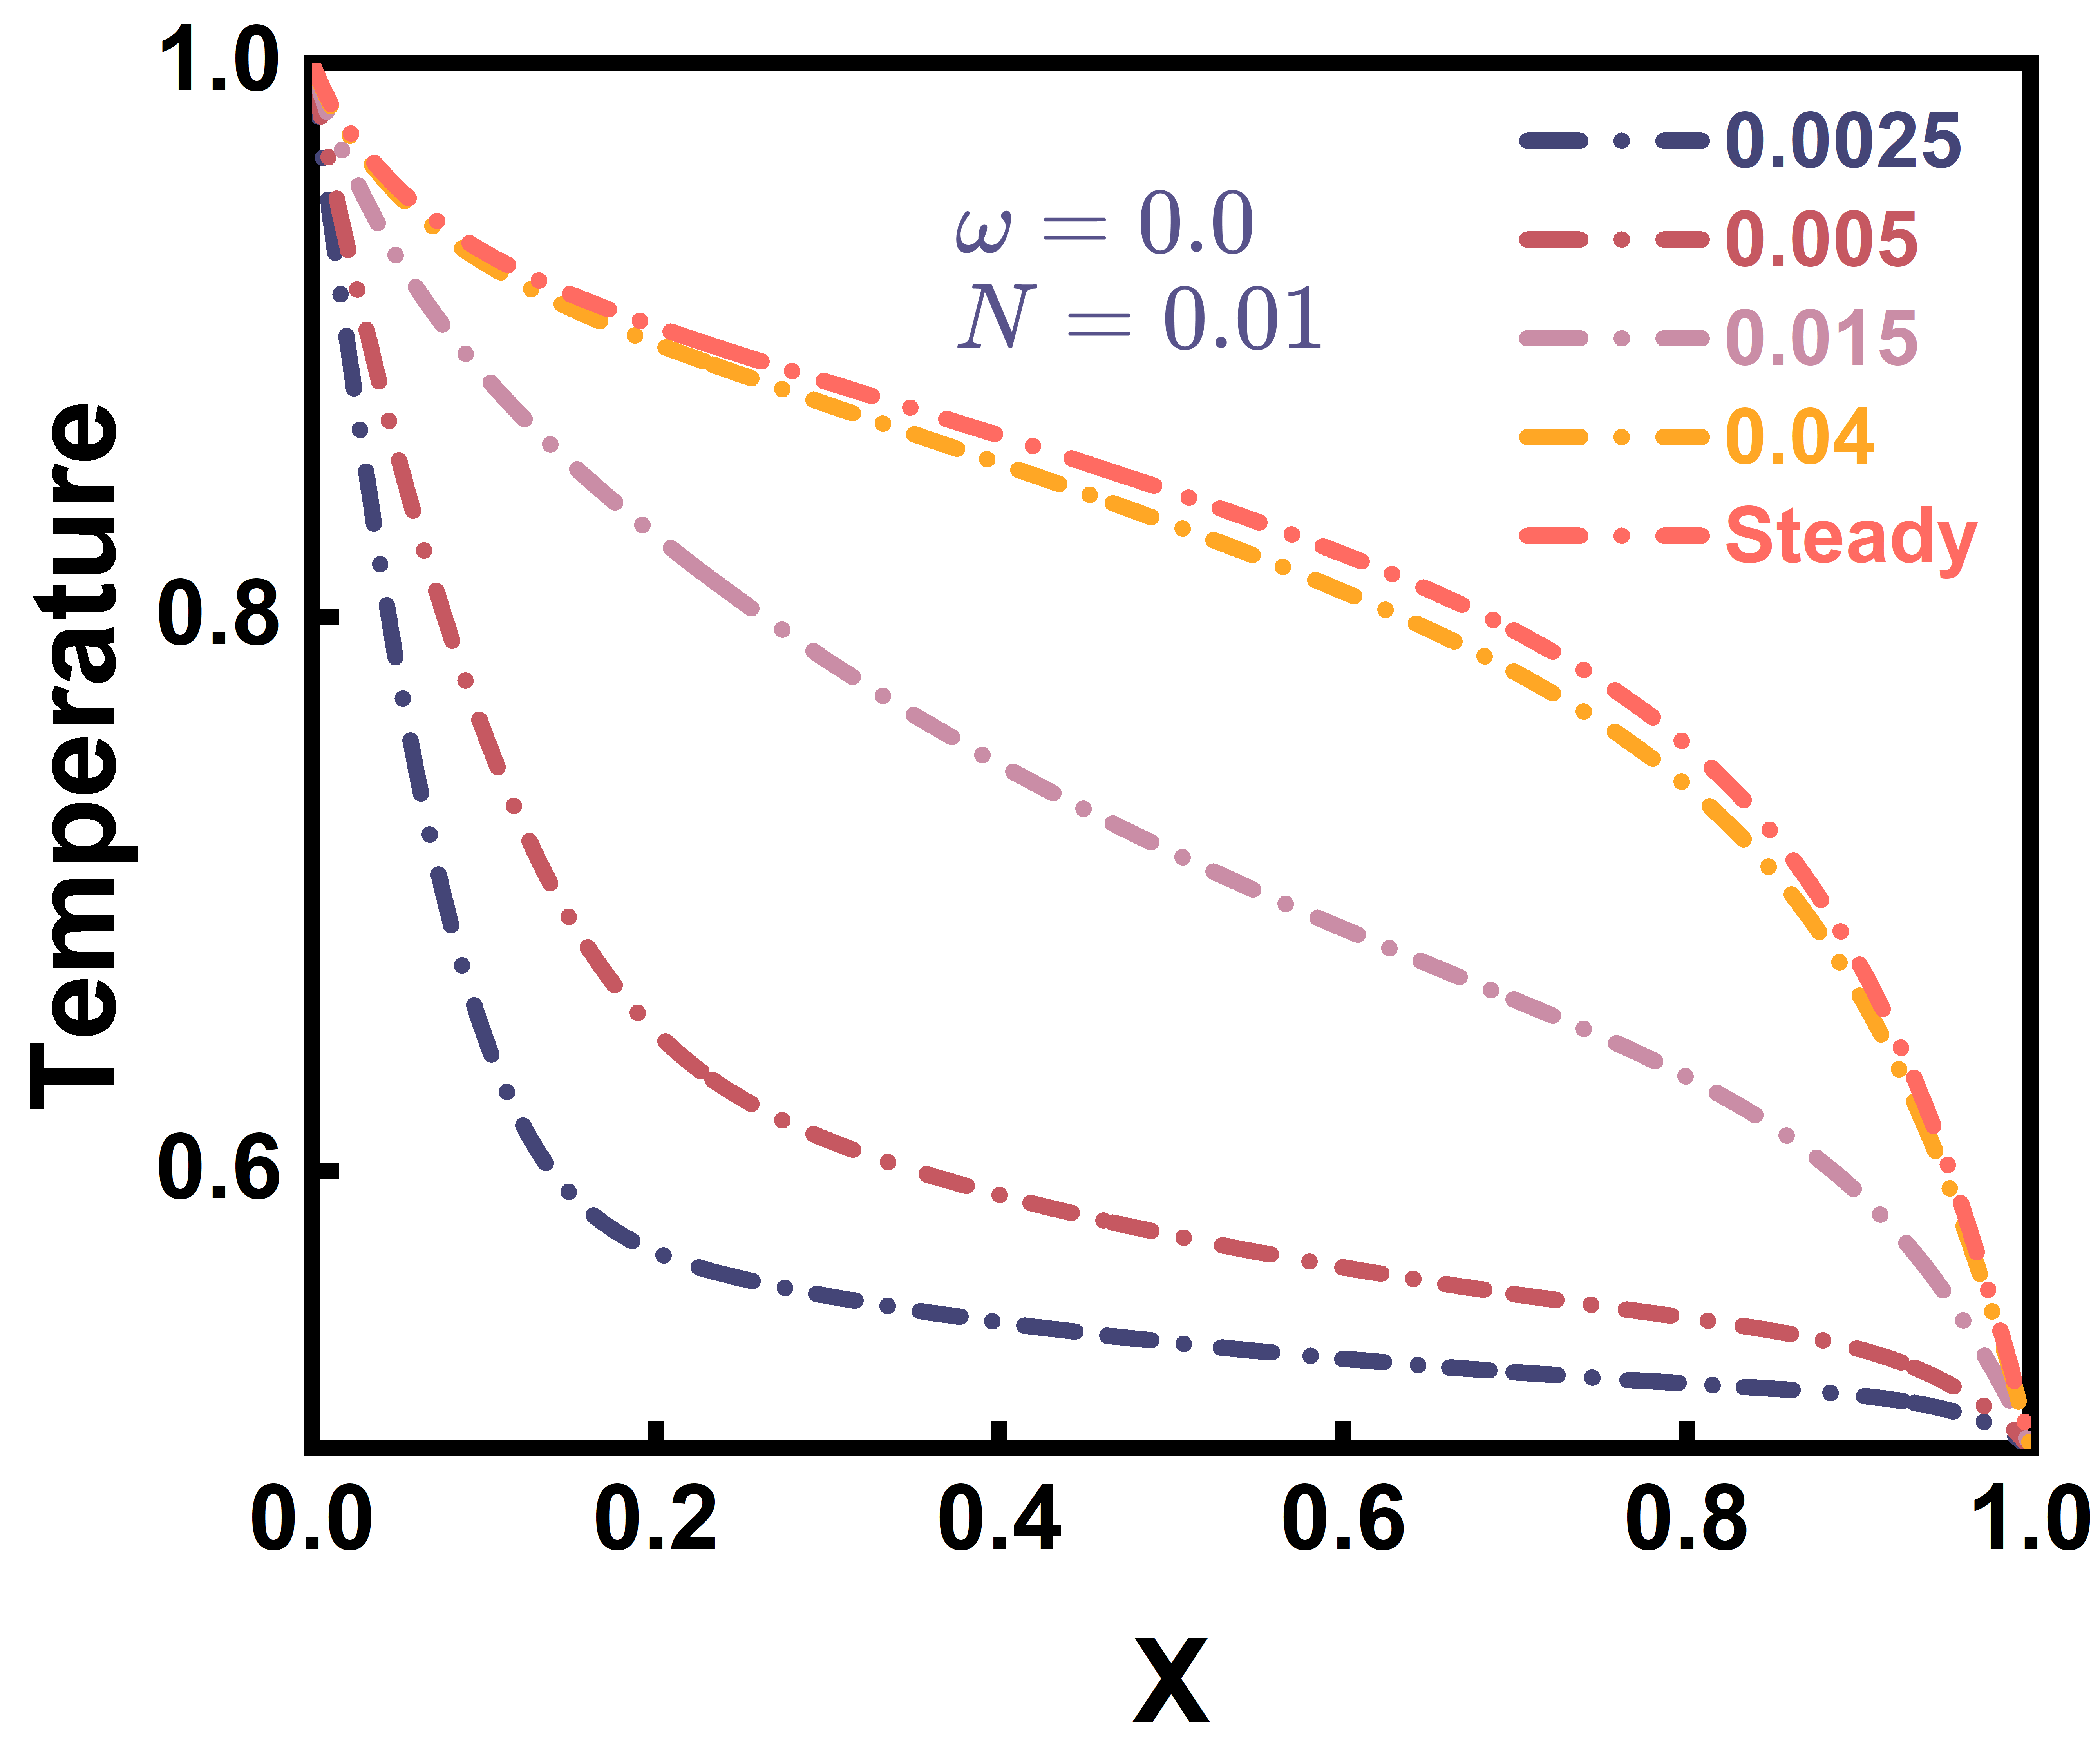
\includegraphics[width=\textwidth]{2A.png}
\caption{}
\end{subfigure}
\hfill
\begin{subfigure}[b]{\figwidth}
\centering
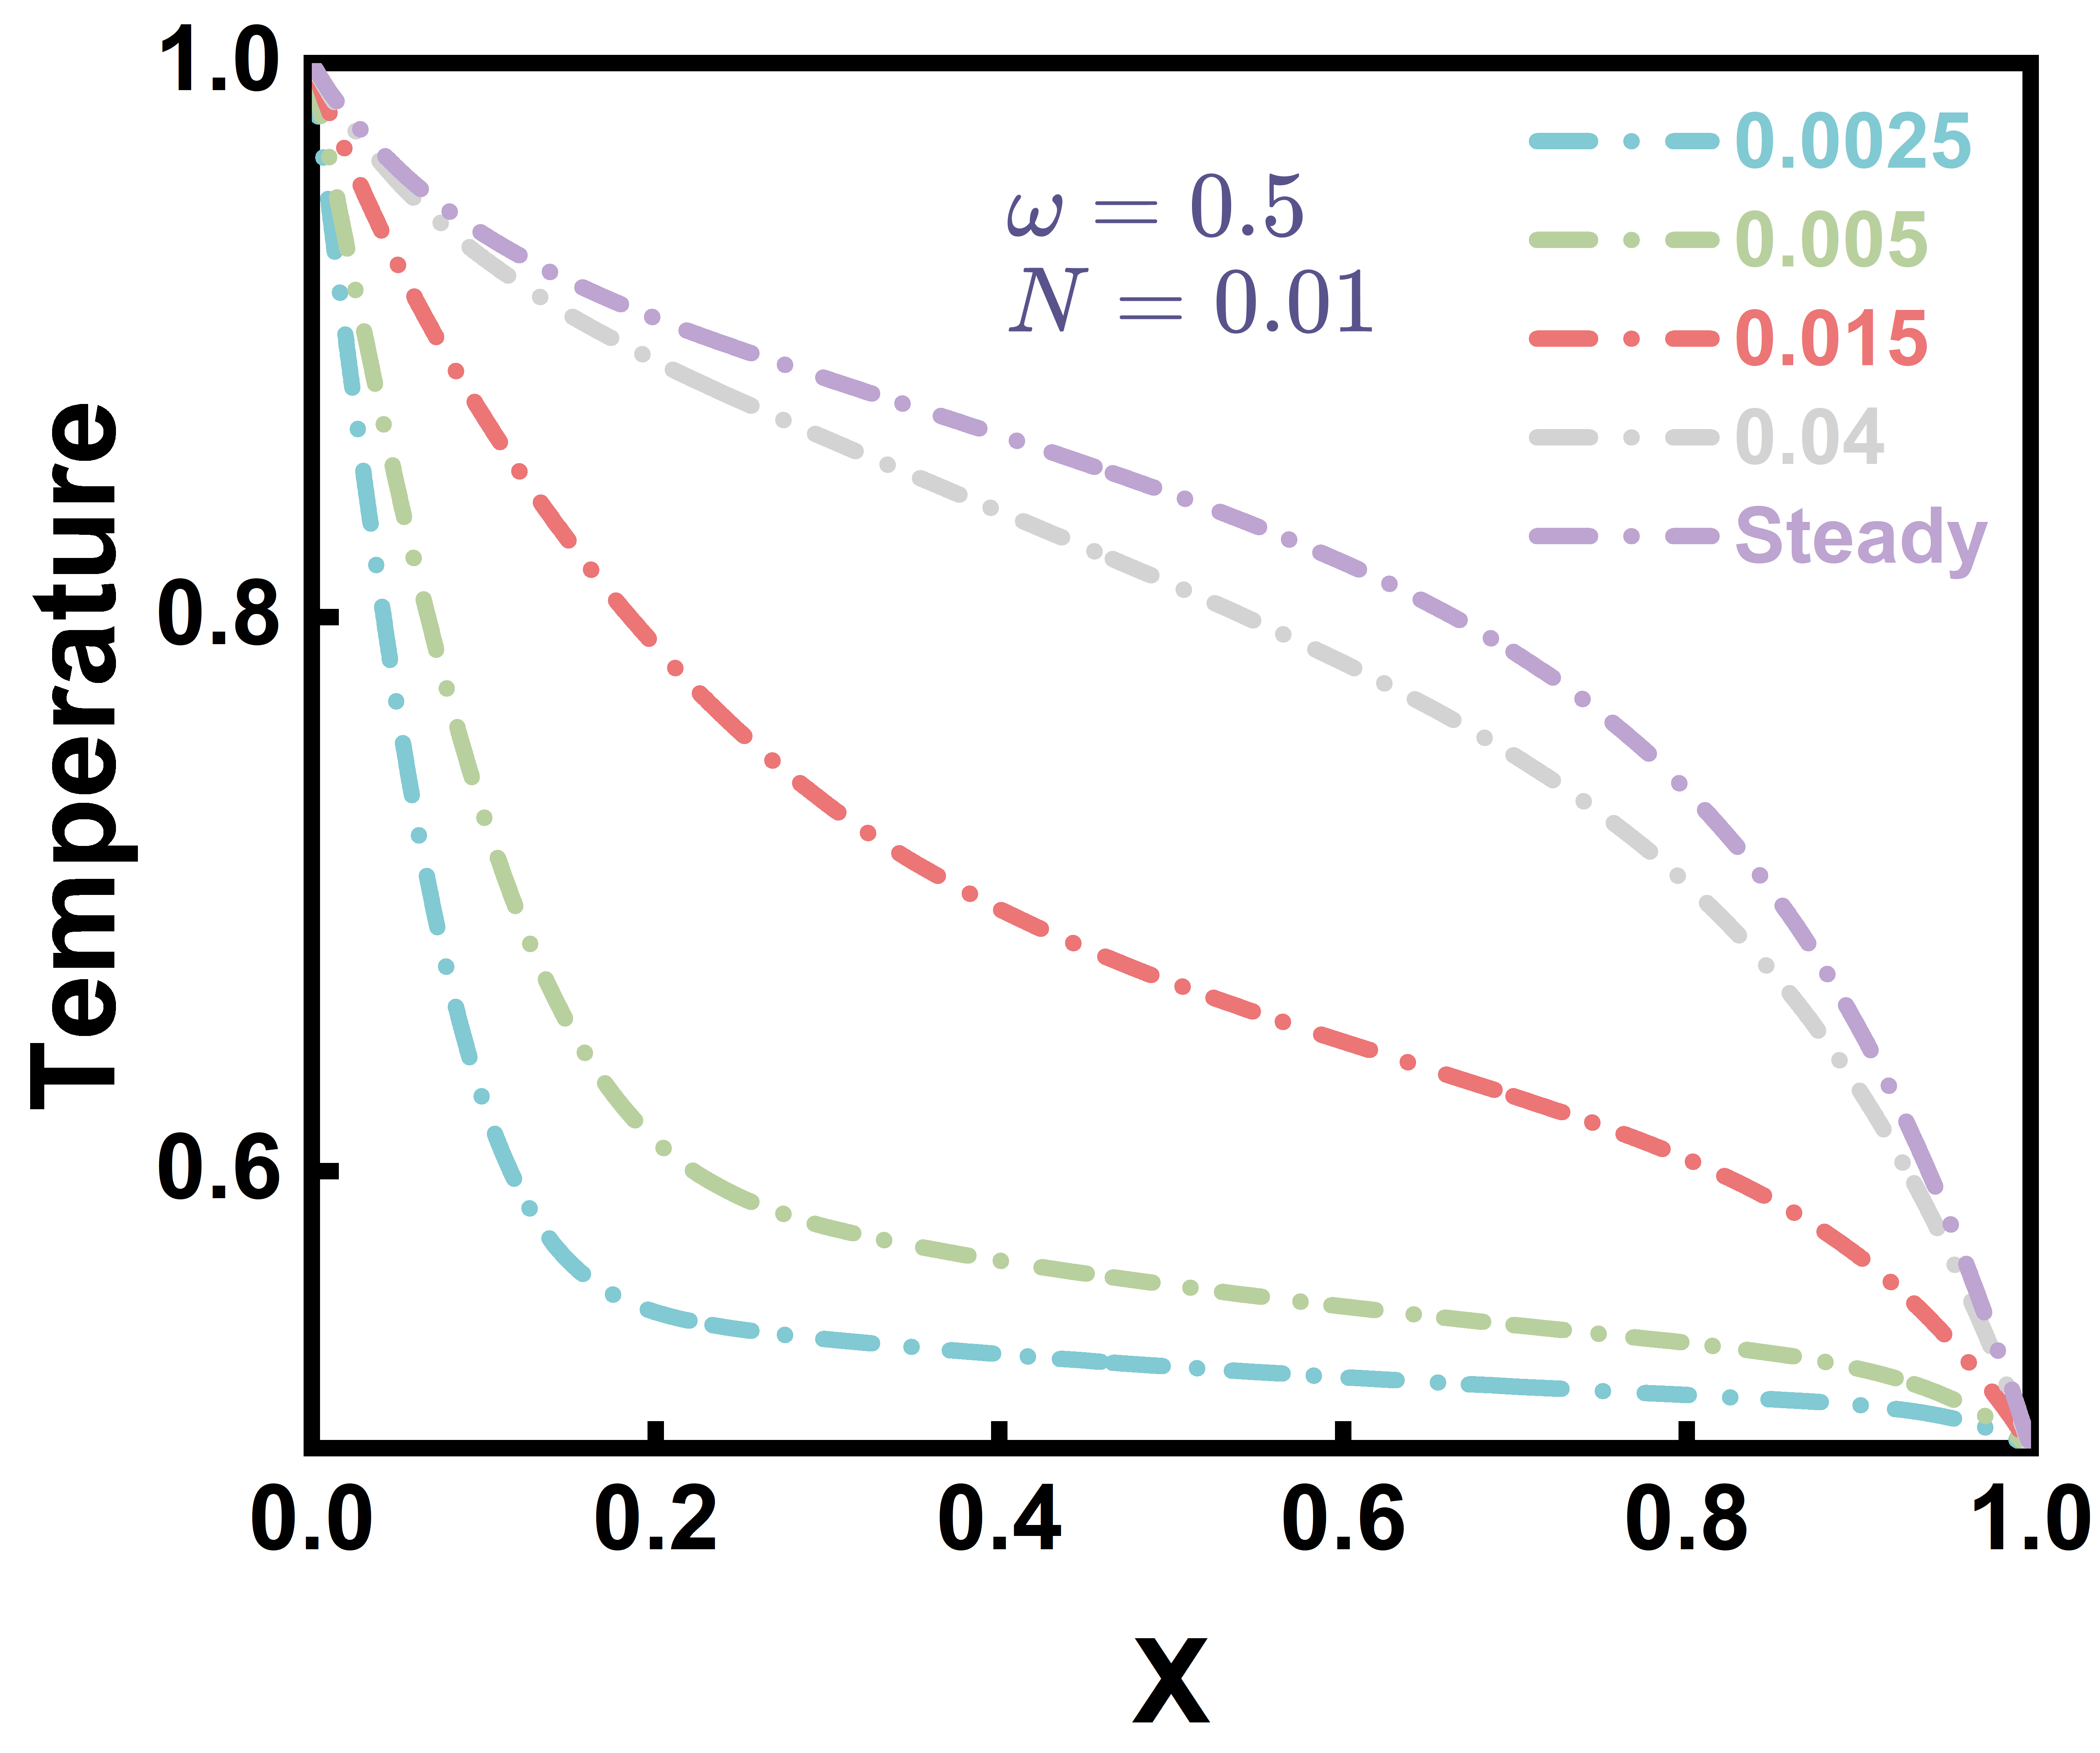
\includegraphics[width=\textwidth]{2B.png}
\caption{}
\end{subfigure}
\hfill
\begin{subfigure}[b]{\figwidth}
\centering
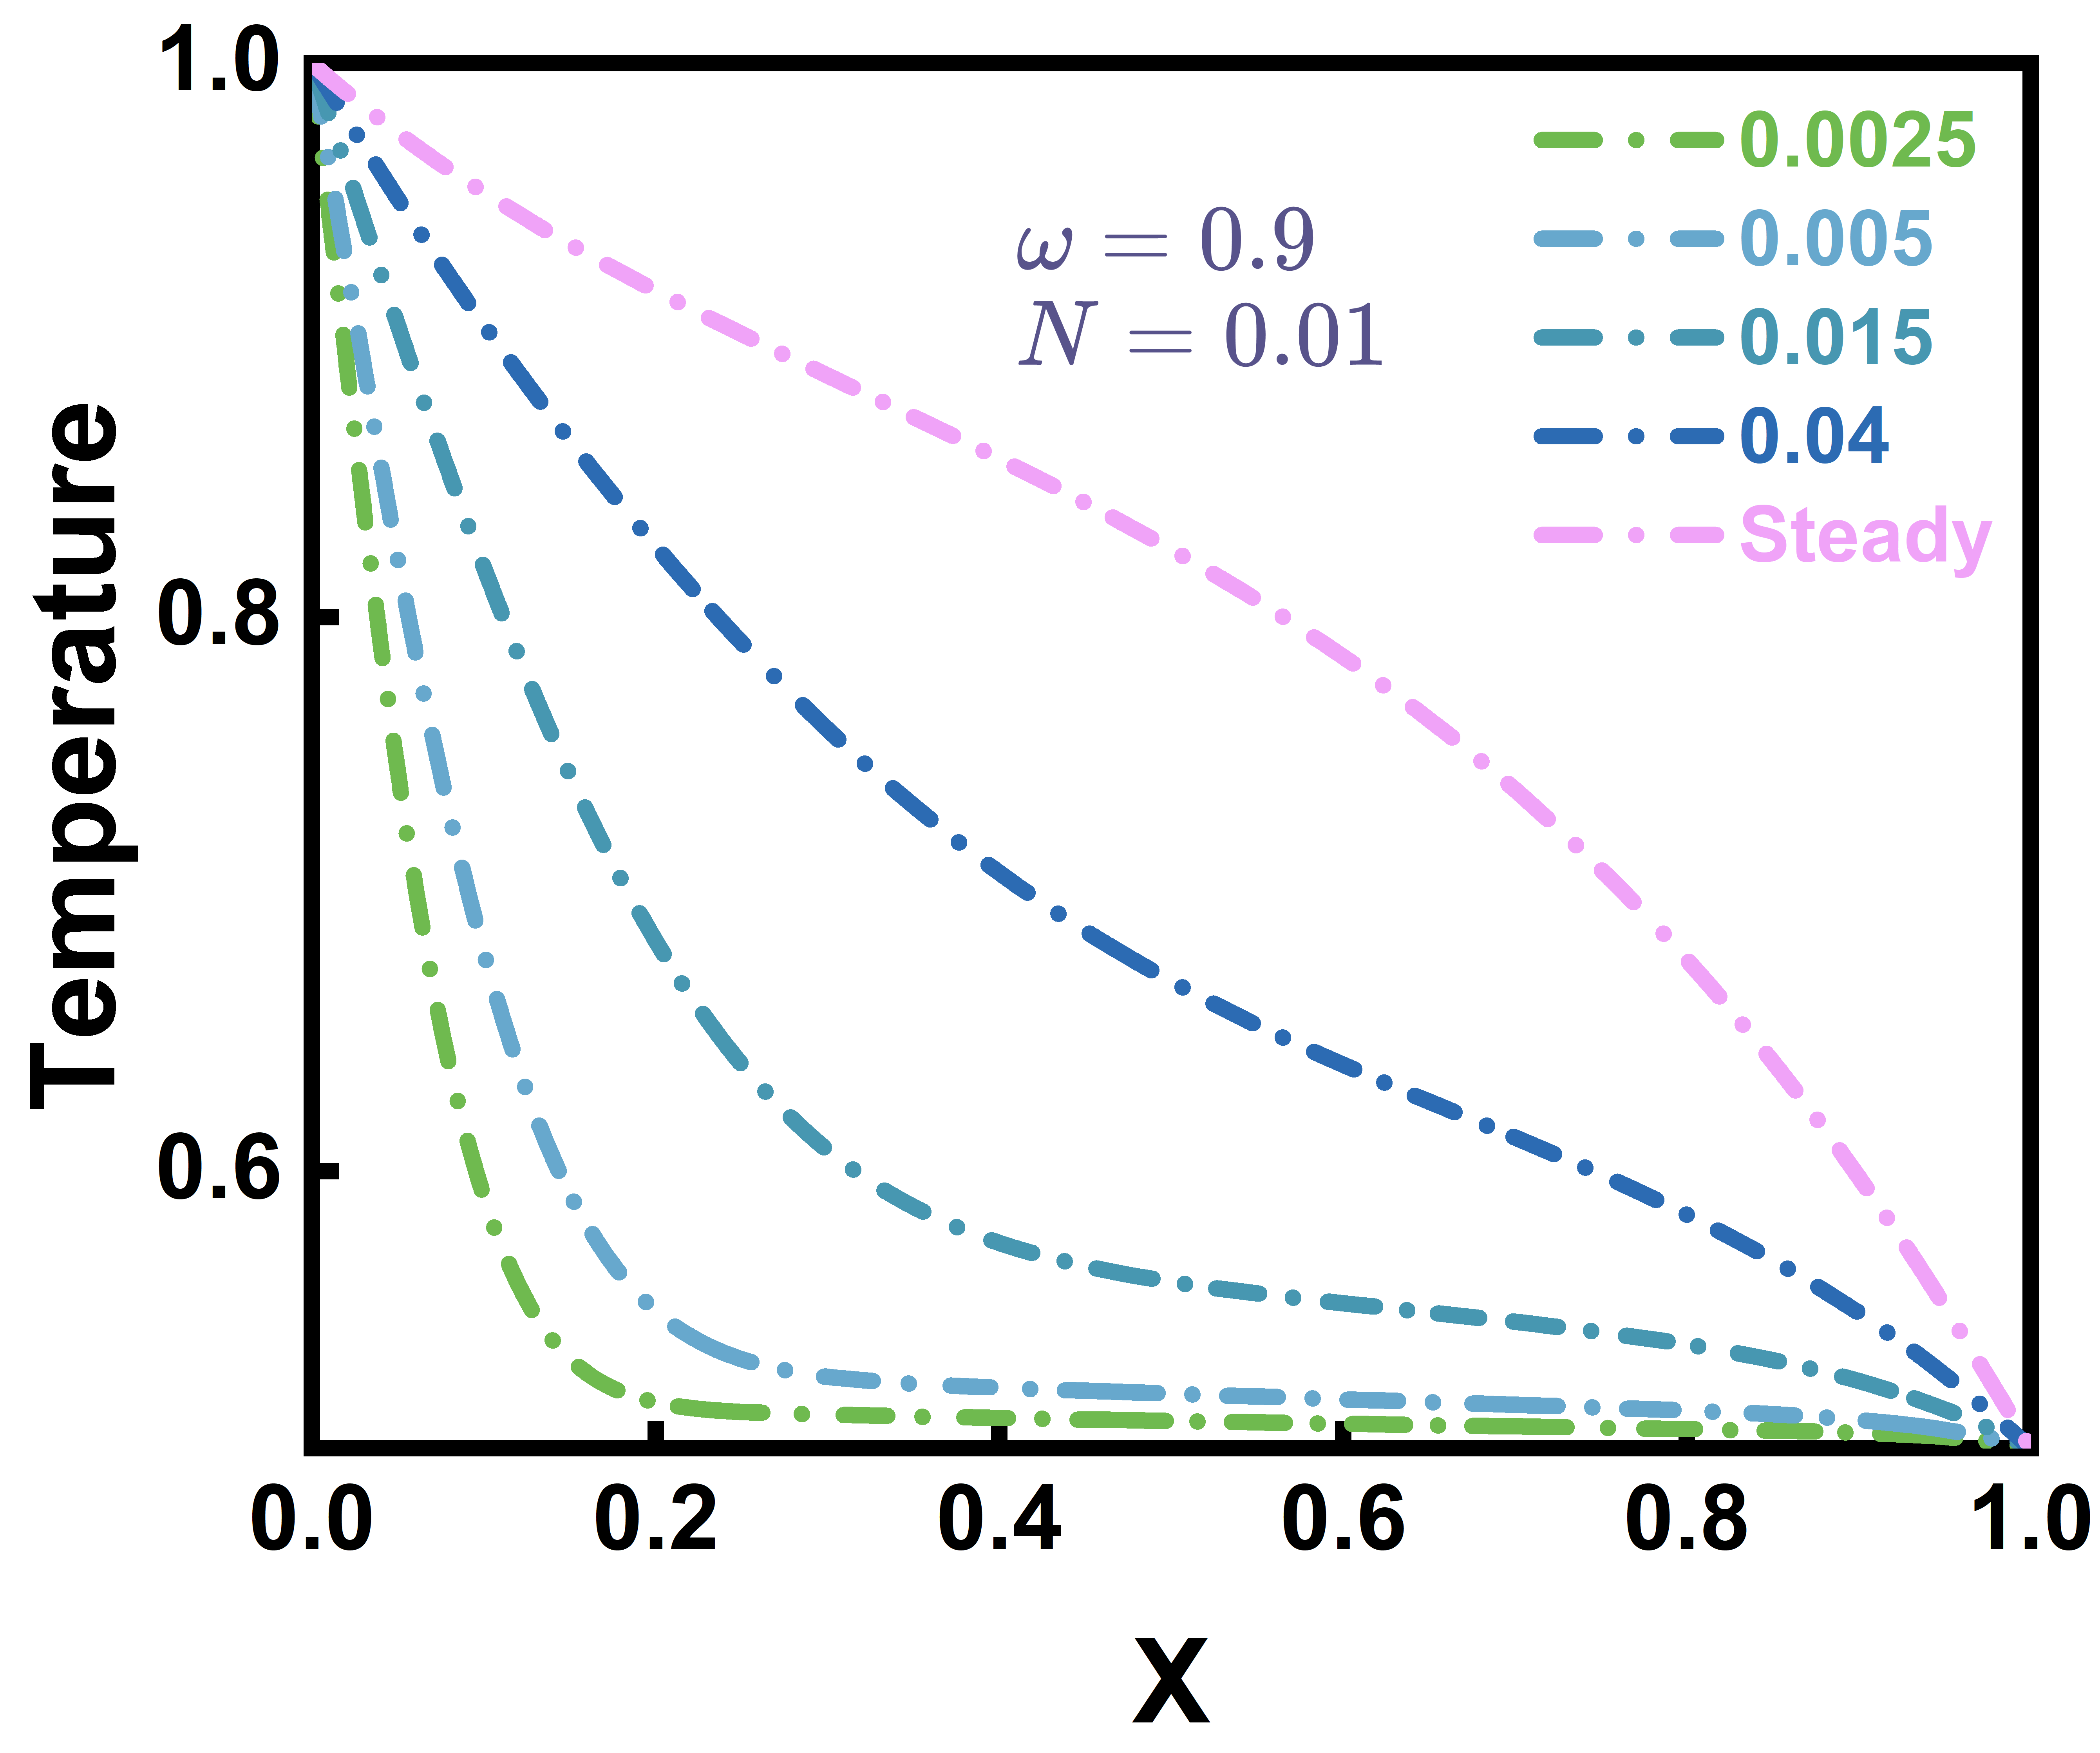
\includegraphics[width=\textwidth]{2C.png}
\caption{}
\end{subfigure}
\caption{Transient dimensionless temperature profiles in a one-dimensional participating slab at $N=0.01$. The scattering albedo is (a) $\omega=0$, (b) $\omega=0.5$,(c) $\omega=0.9$.}
\label{fig2}
\end{figure}

Figure~\ref{fig2} shows the transient temperature profiles at $N=0.01$. The profile was strongly nonlinear at $\omega=0$, and the interior temperature rose rapidly after heating began. Increasing $\omega$ to $0.5$ and $0.9$ lowered the temperature throughout the slab. It also increased the time required to approach steady state. The temperature remained nonlinear while the medium retained a non-zero absorbing component.

\begin{figure}[H]
\centering
\begin{subfigure}[b]{\figwidth}
\centering
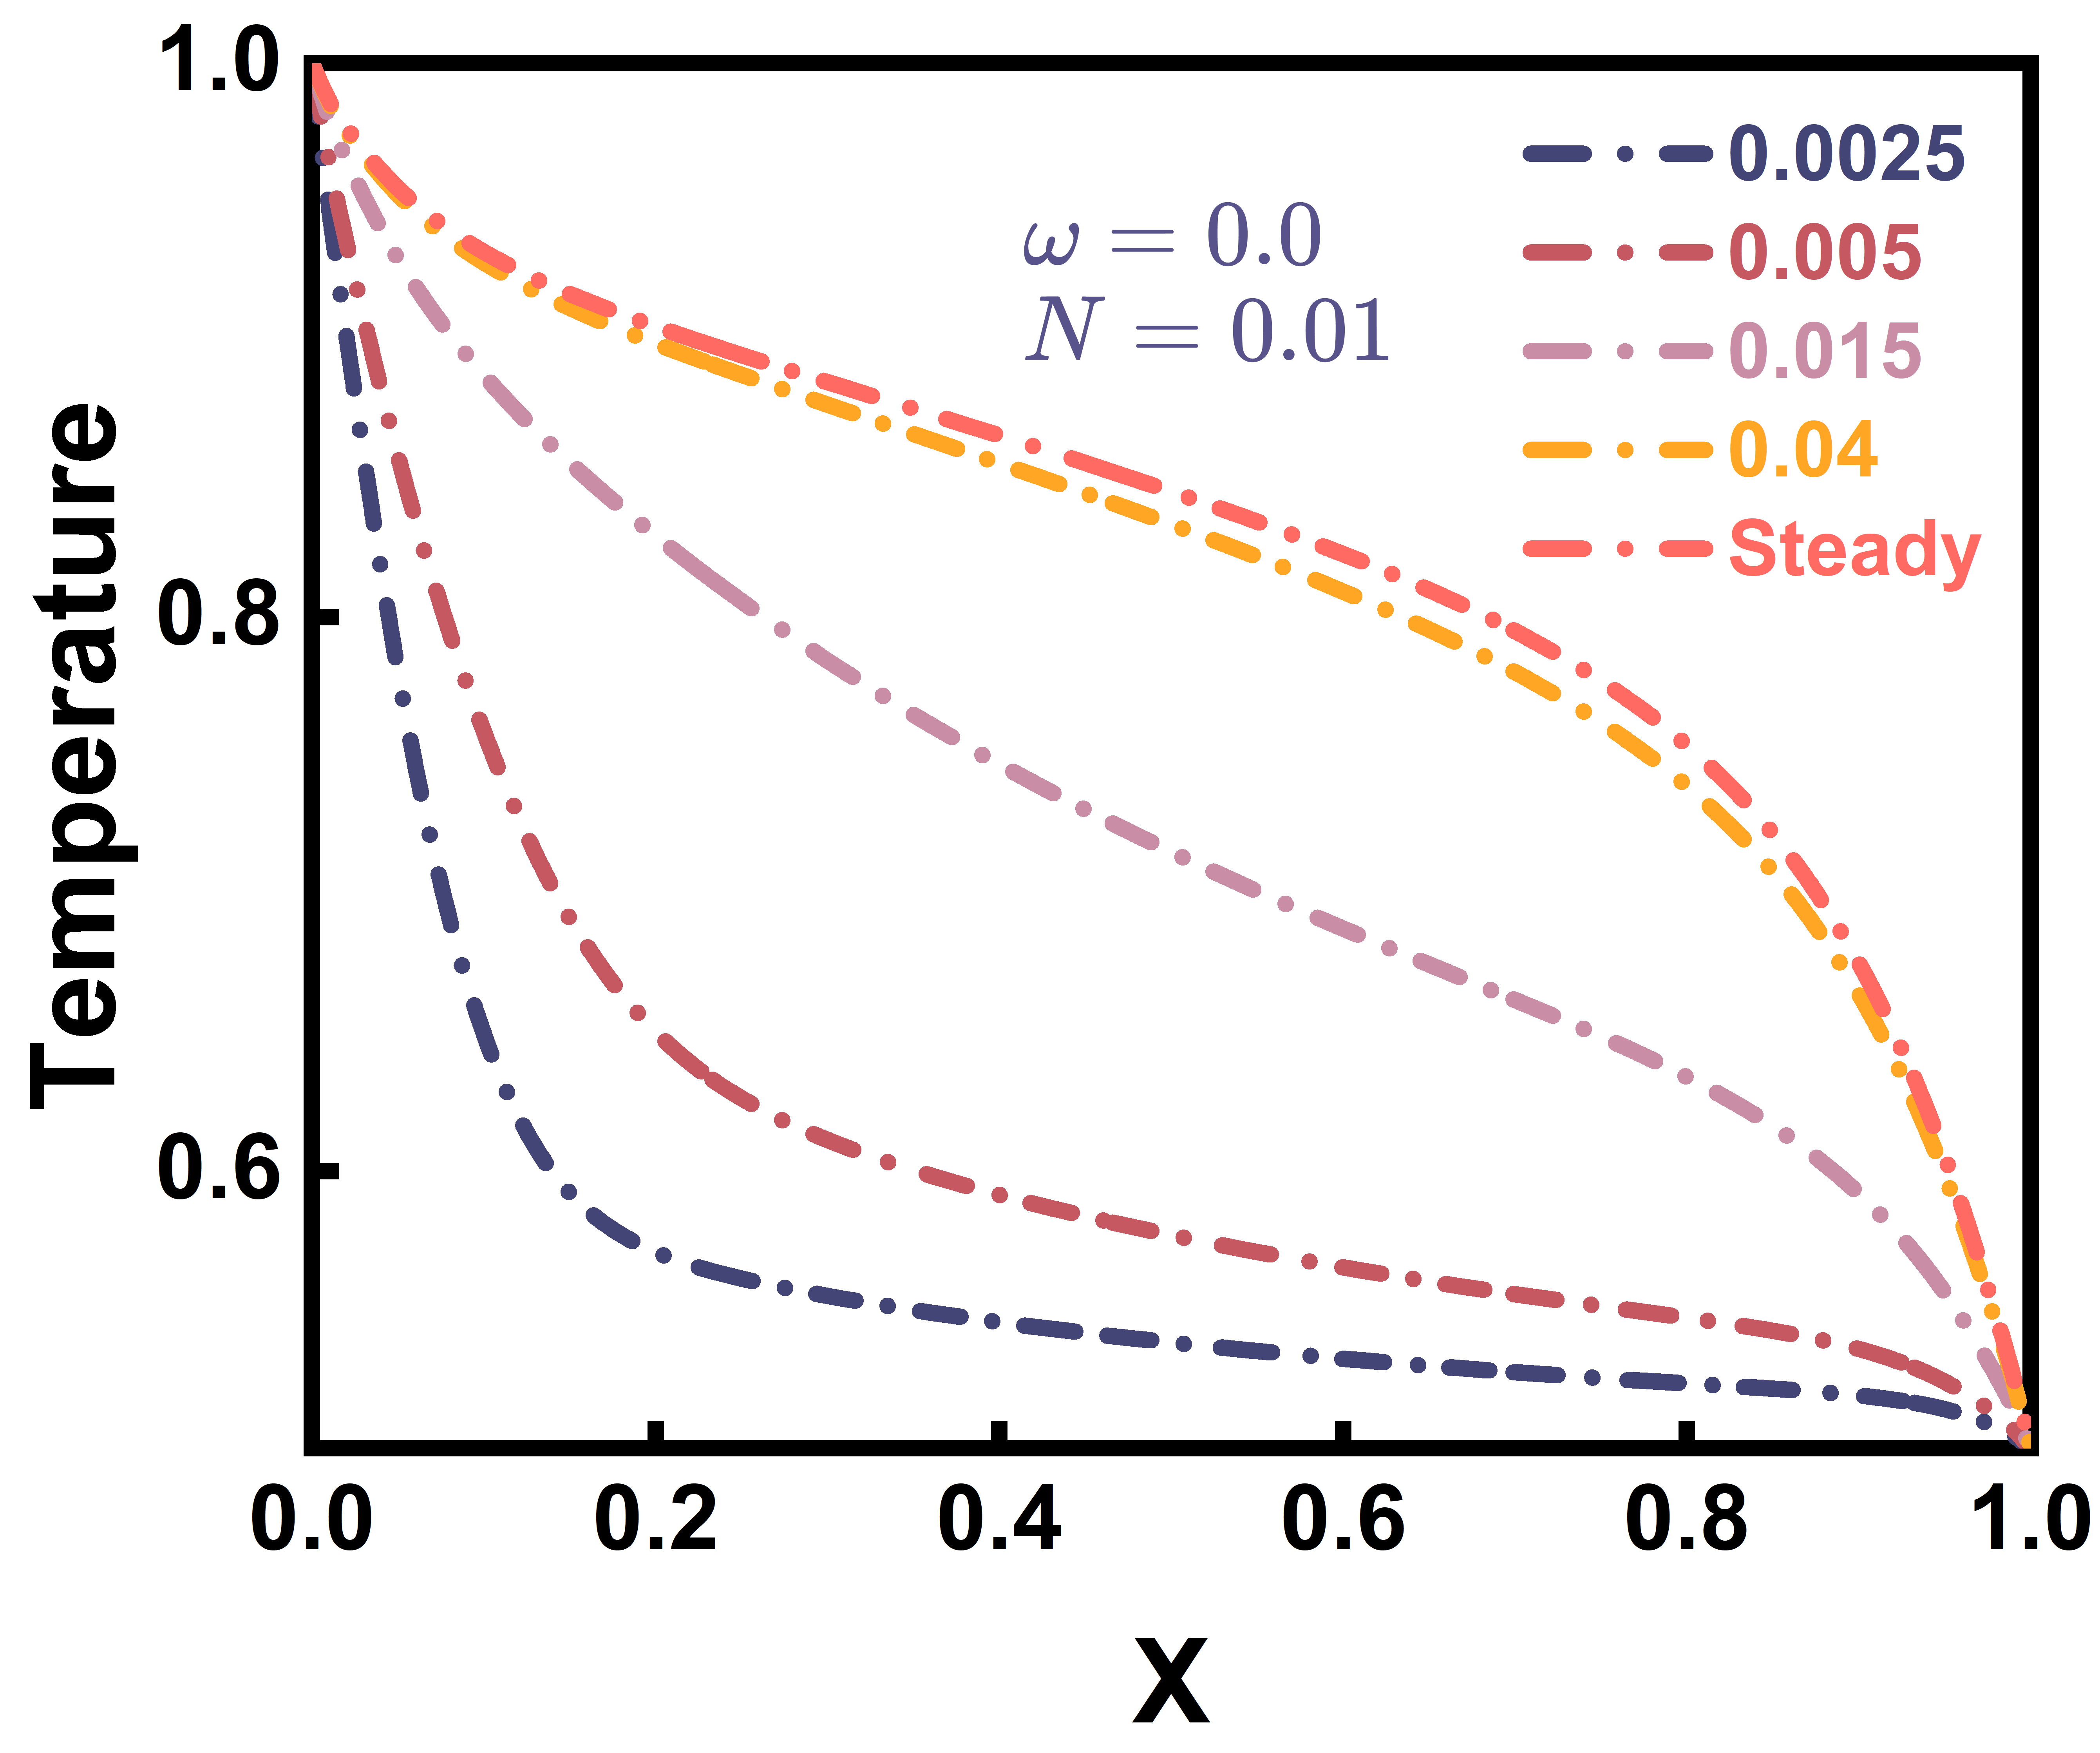
\includegraphics[width=\textwidth]{3A.png}
\caption{}
\end{subfigure}
\hfill
\begin{subfigure}[b]{\figwidth}
\centering
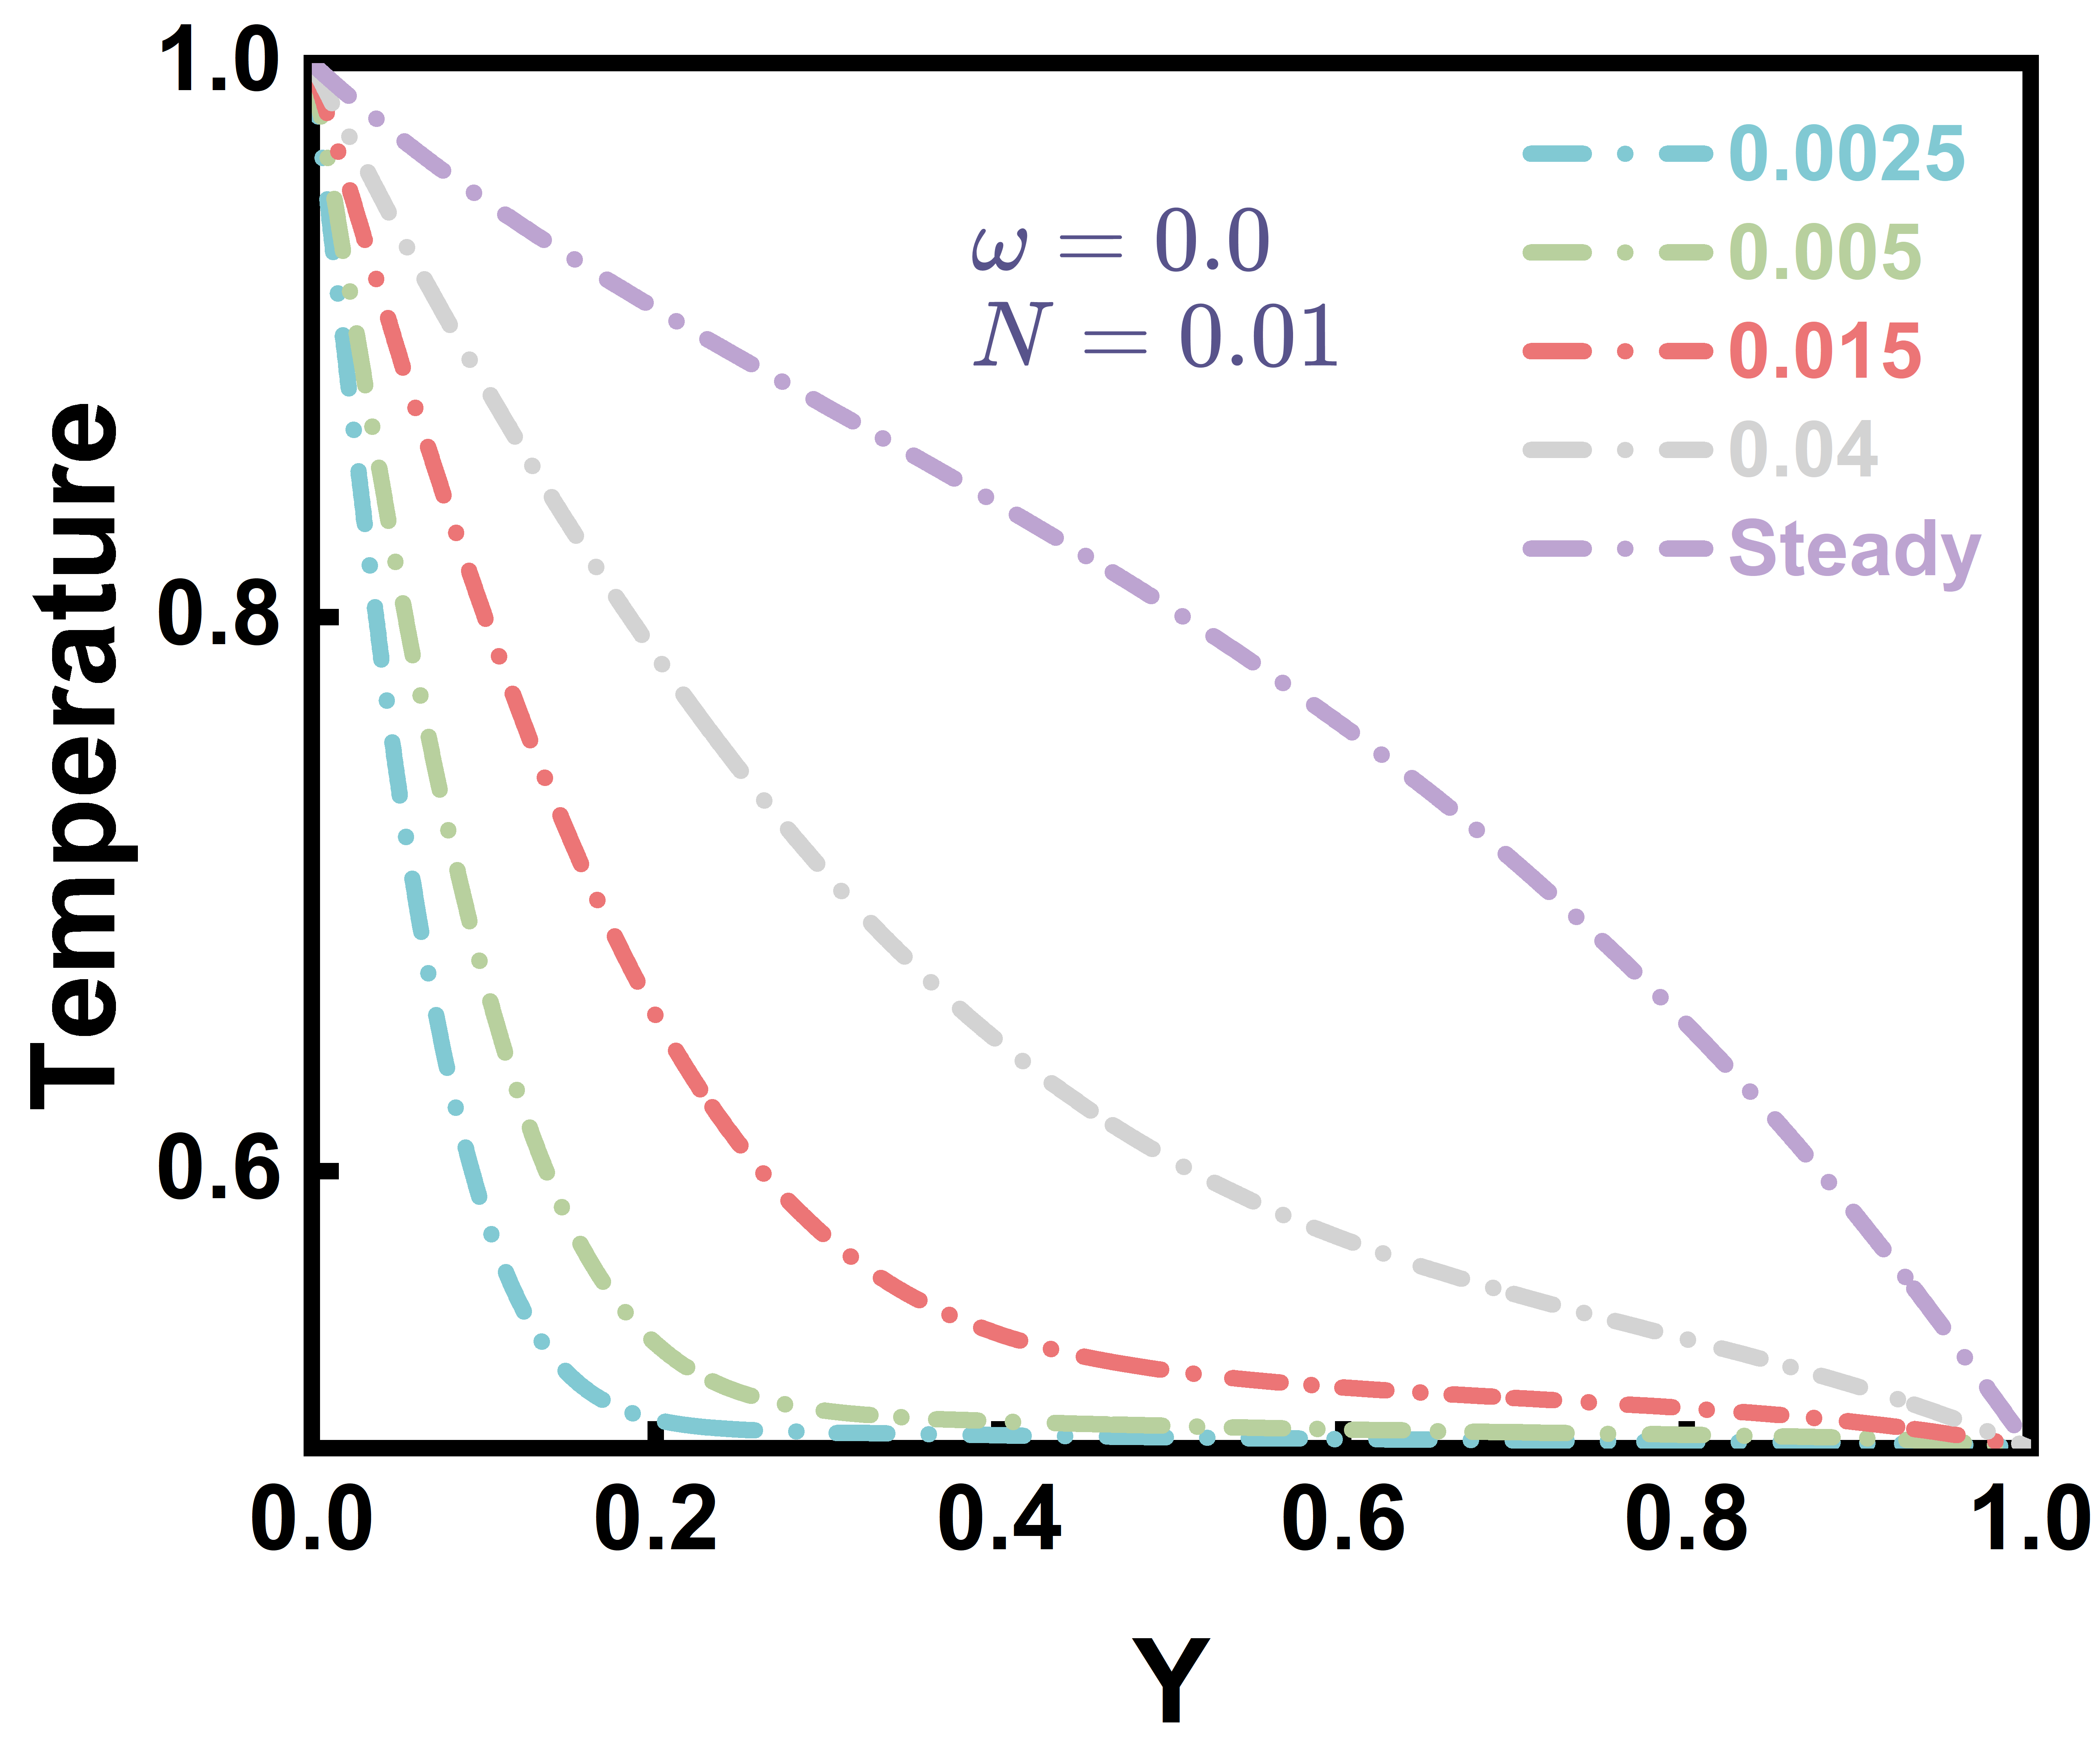
\includegraphics[width=\textwidth]{3B.png}
\caption{}
\end{subfigure}
\hfill
\begin{subfigure}[b]{\figwidth}
\centering
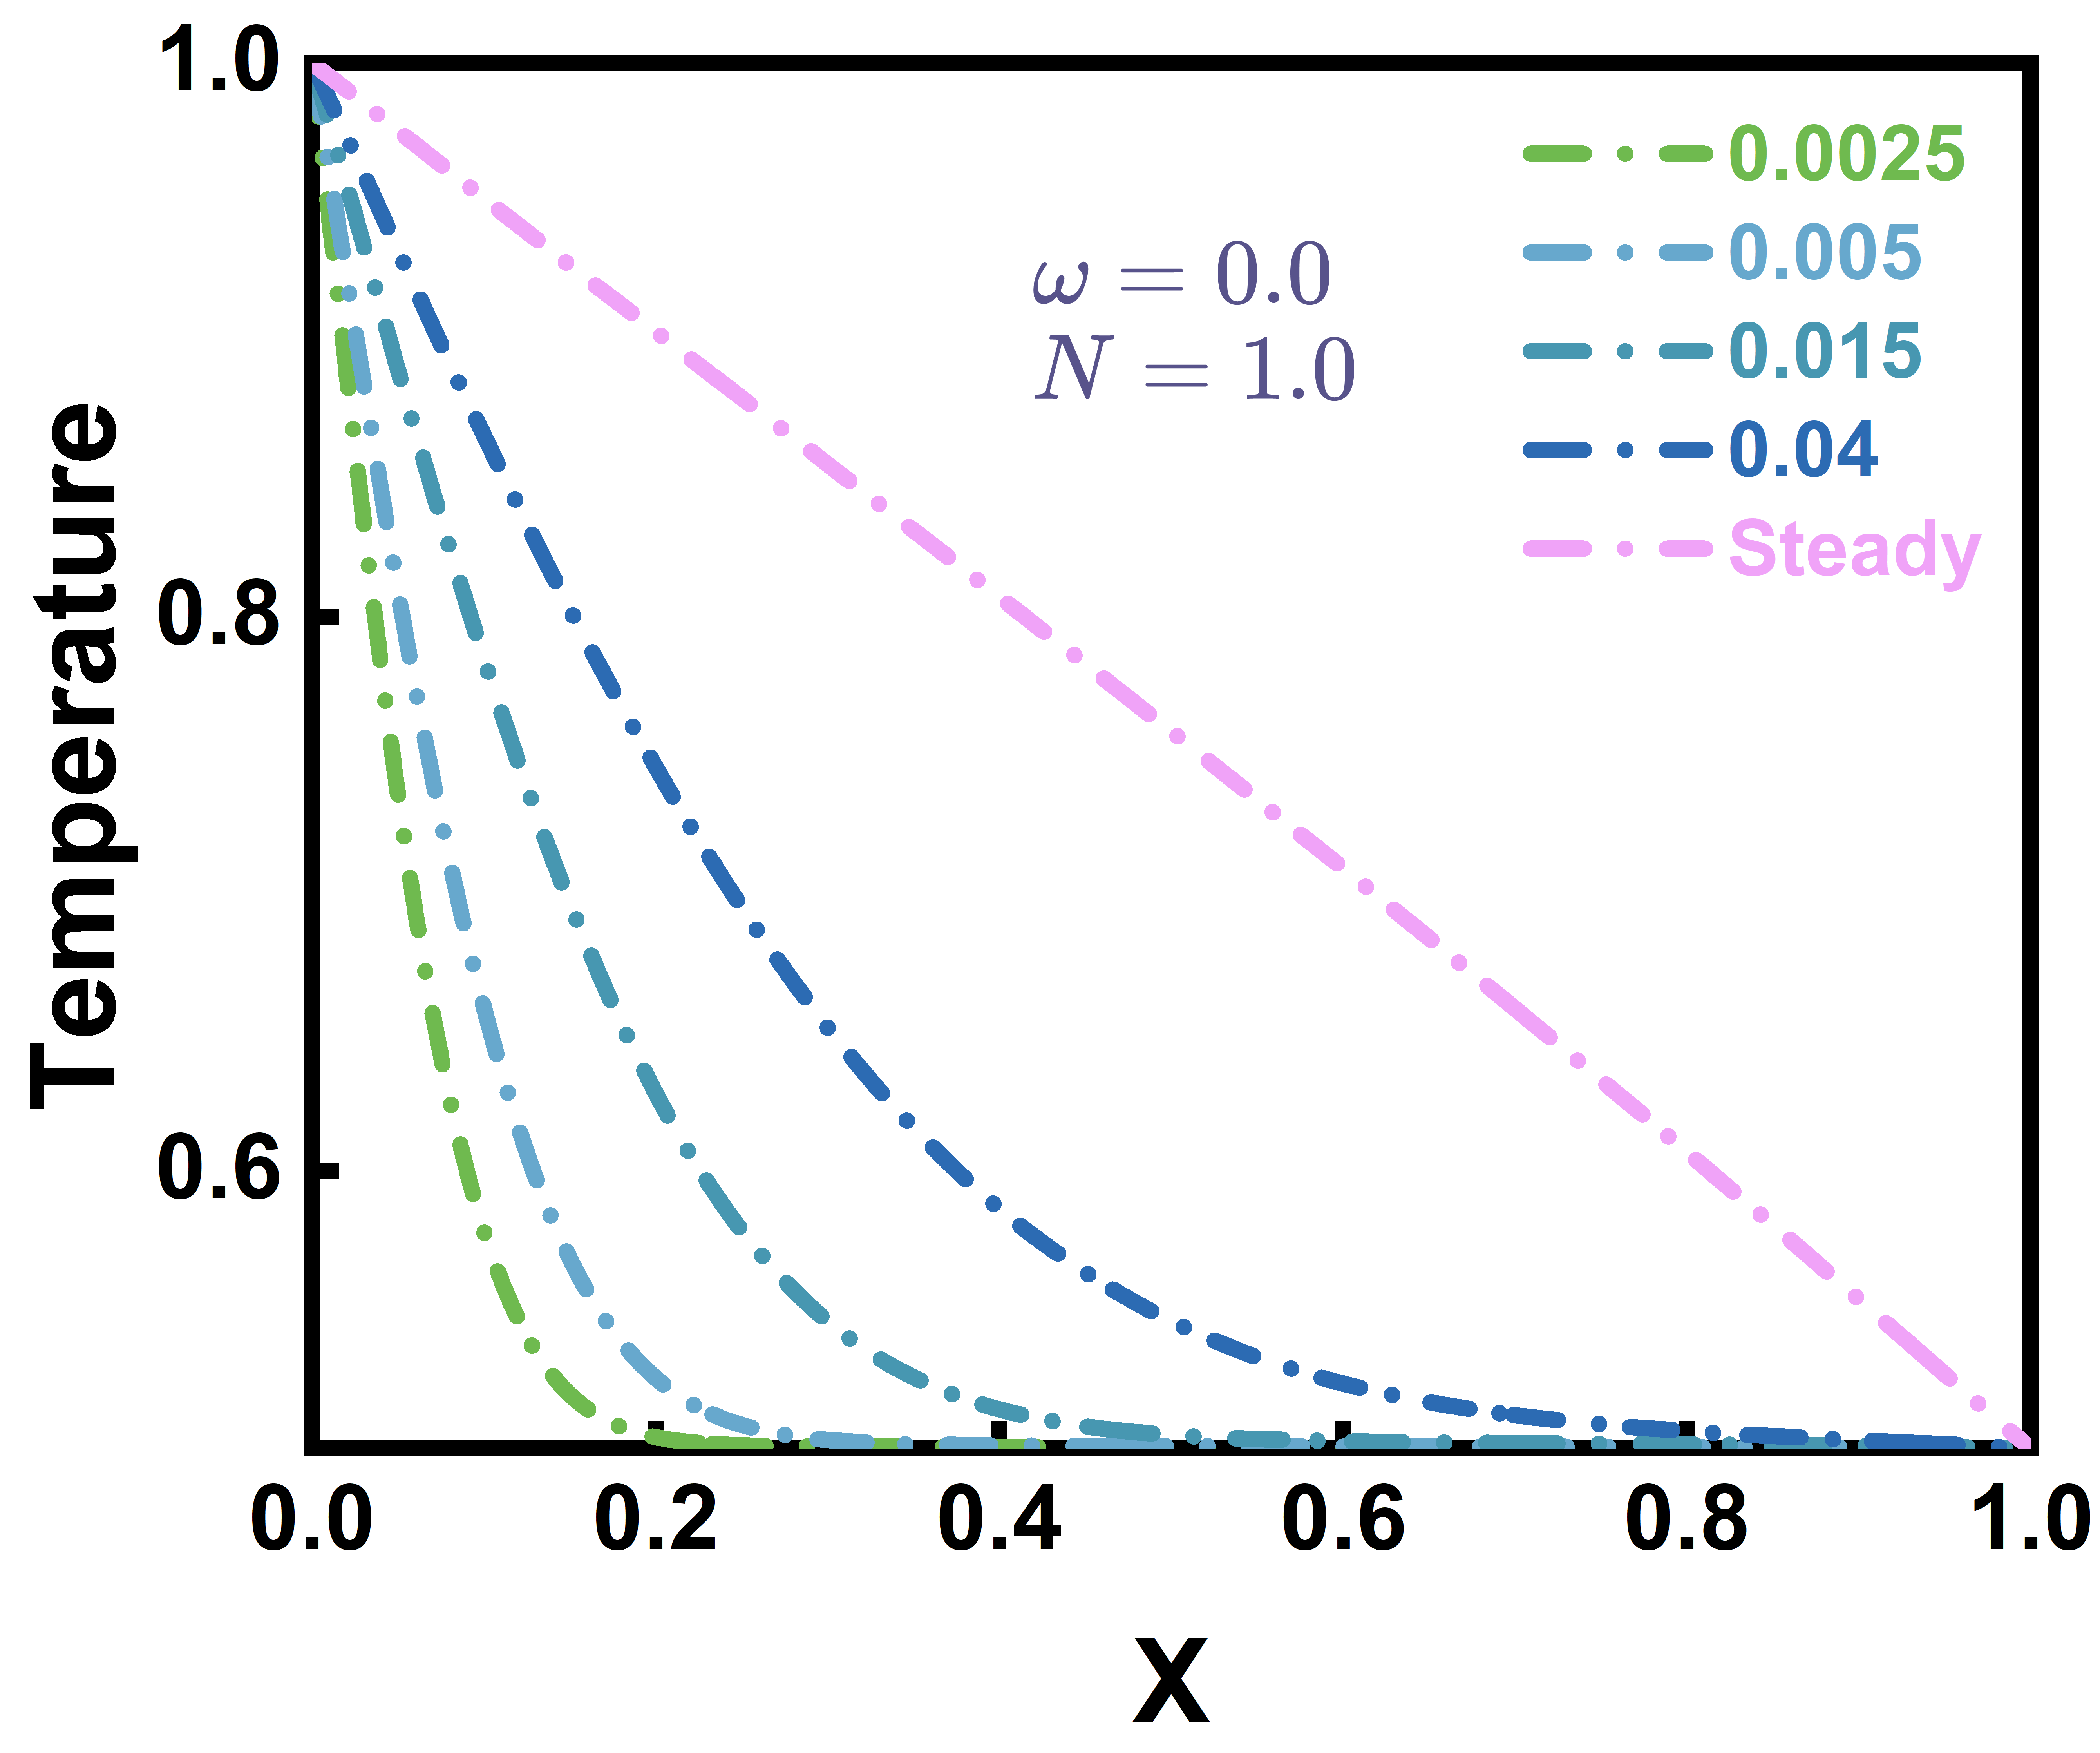
\includegraphics[width=\textwidth]{3C.png}
\caption{}
\end{subfigure}
\caption{Transient dimensionless temperature profiles in a one-dimensional participating slab at $\omega=0$. The conduction--radiation parameter is (a) $N=0.01$, (b) $N=0.10$,(c) $N=1.00$.}
\label{fig3}
\end{figure}

Figure~\ref{fig3} compares transient temperature profiles for different values of $N$. At $N=0.01$, the slab heated rapidly and retained a strongly nonlinear steady-state profile. The curves at $N=0.10$ lay between the radiation-dominated and conduction-dominated limits. At $N=1.00$, early heating remained concentrated near the hot wall, and the steady-state profile approached a linear distribution. Increasing $N$ therefore lowered the slab temperature and delayed thermal penetration towards the cold wall.

Figure~\ref{fig4} reports the flux profiles at $\zeta=0.005$ for $N=0.10$, $T_E=0.1$, and unit optical thickness. Conductive flux was obtained from the temperature gradient, whereas radiative flux was calculated from the first angular moment of intensity. Both components contributed at $\omega=0$, while the radiative component decreased as $\omega$ increased. At $\omega=1.0$, the volumetric radiative source vanished and conduction governed the thermal response. The decomposed fluxes agreed with the collapsed-dimension benchmark of Talukdar and Mishra~\cite{Talukdar2001} for the same configuration.

\begin{figure}[H]
\centering
\begin{subfigure}[b]{\figwidth}
\centering
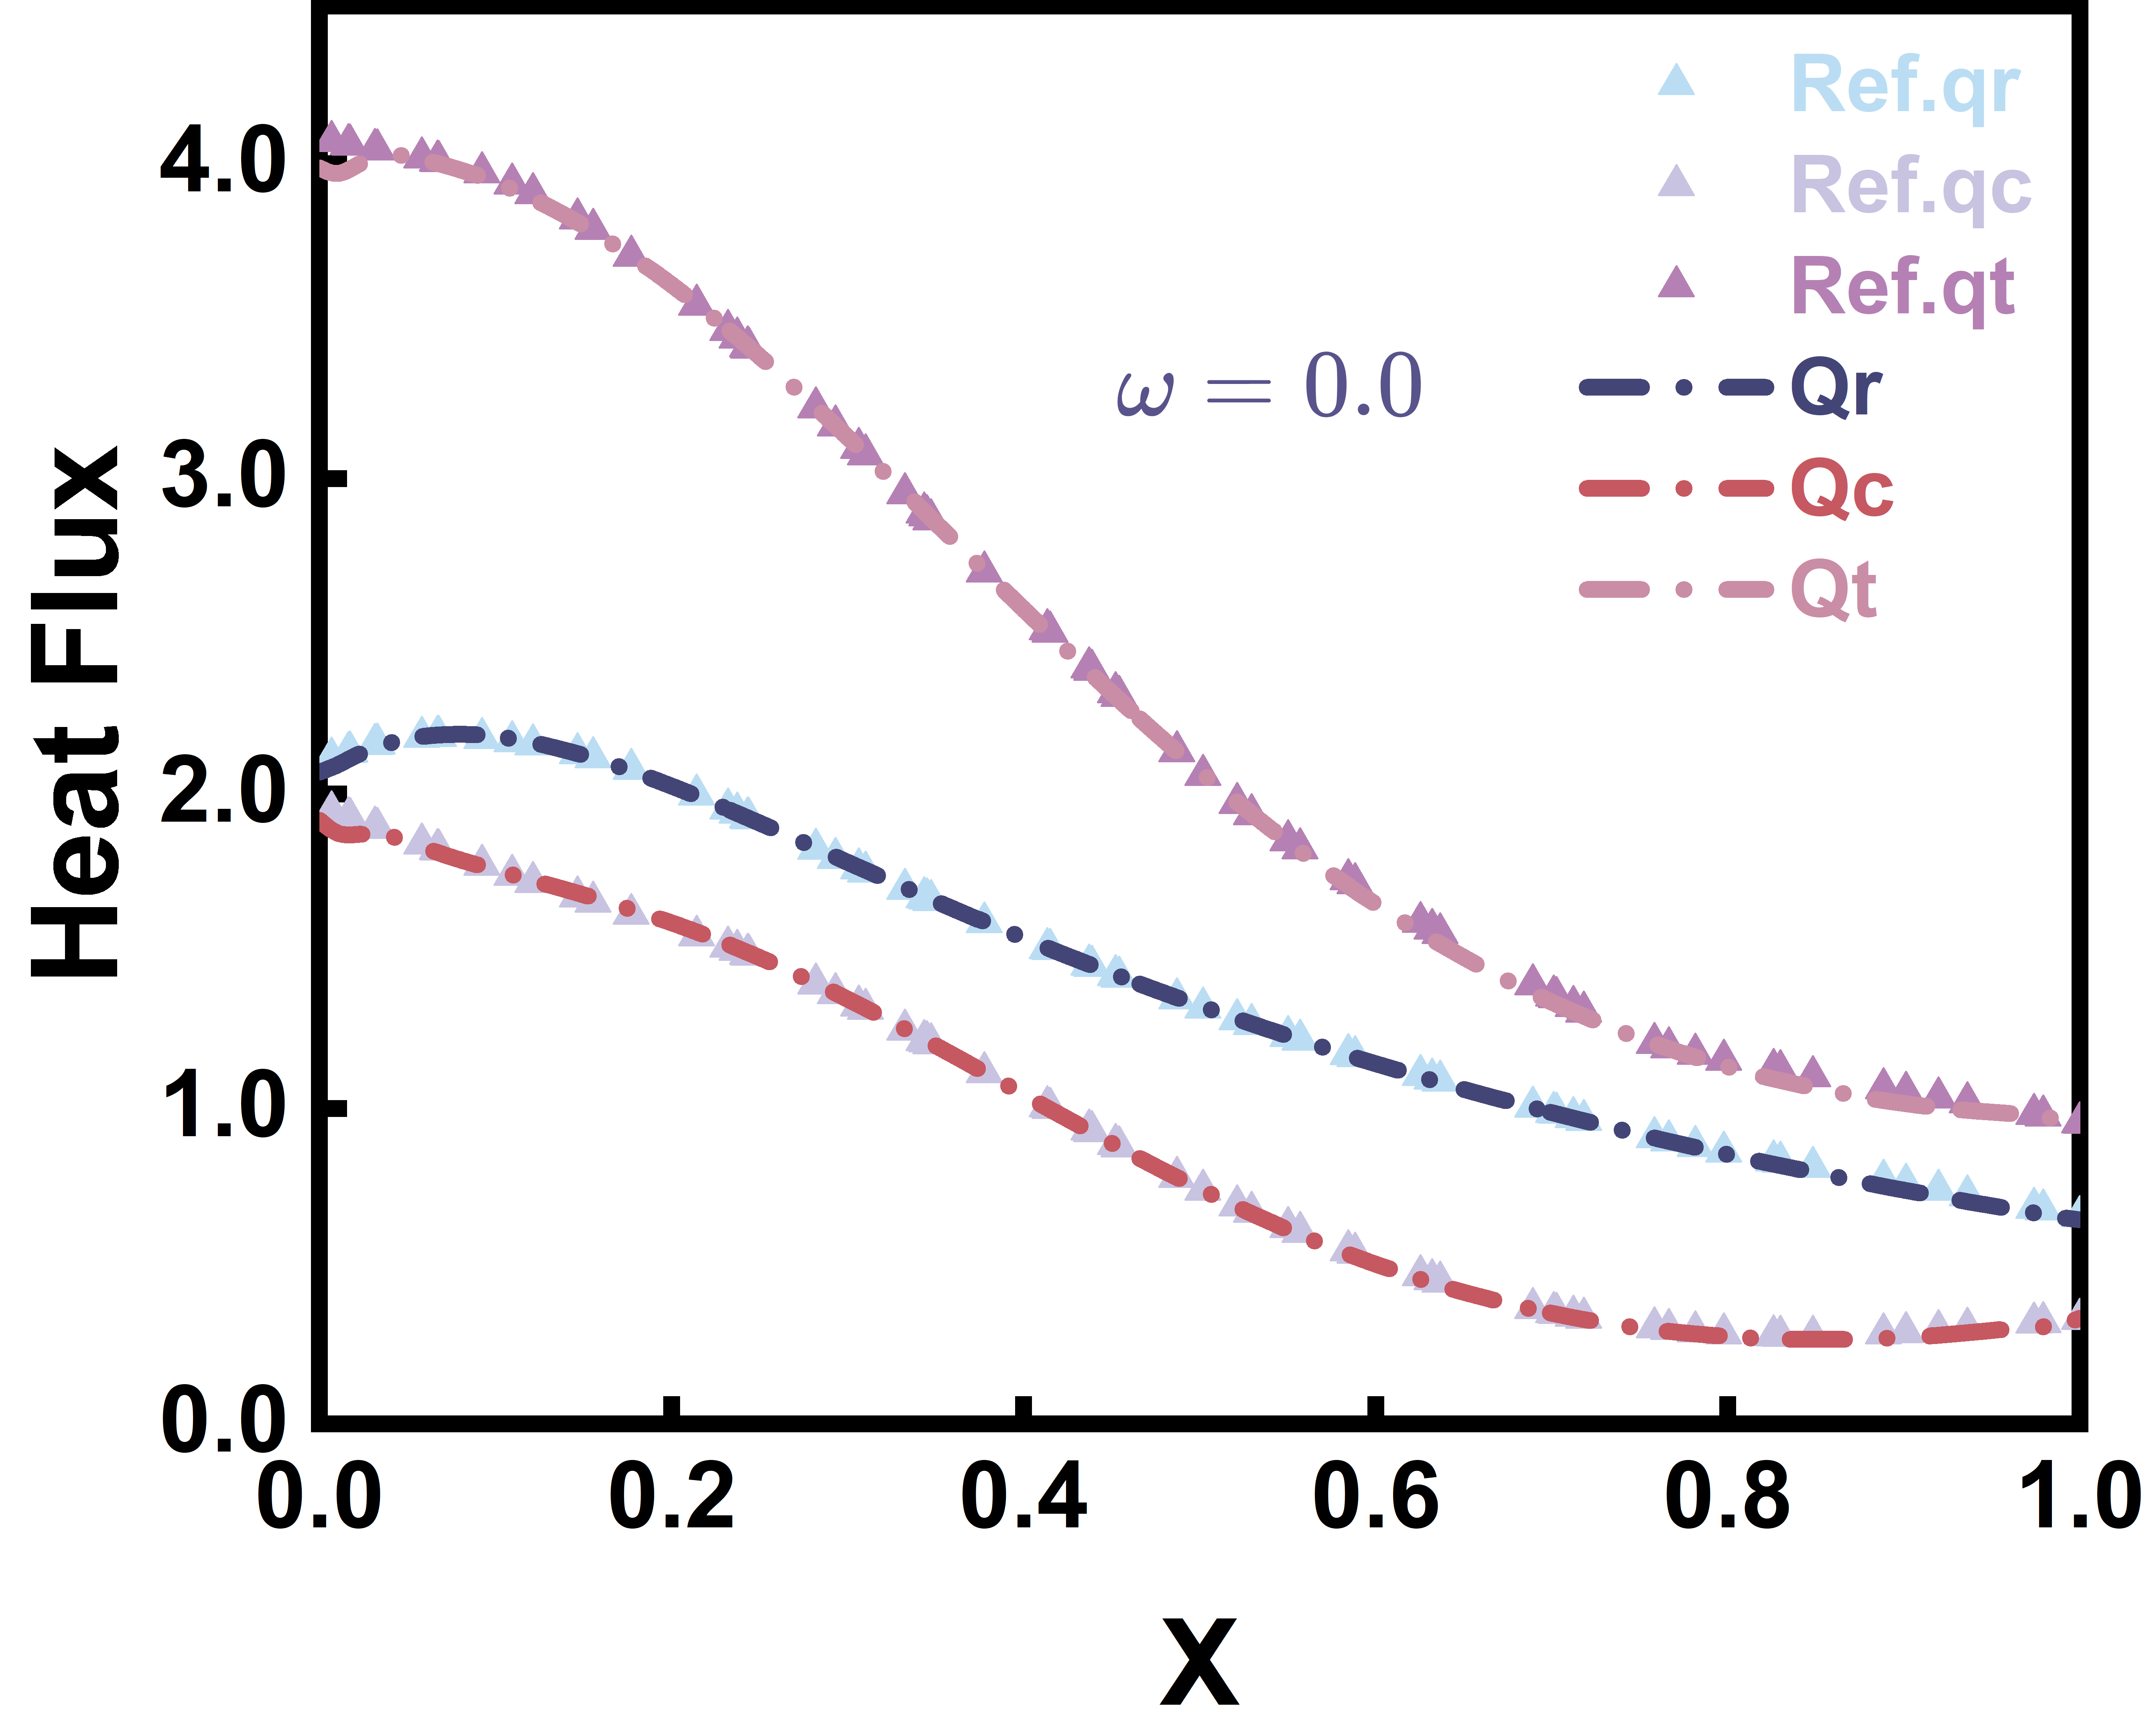
\includegraphics[width=\textwidth]{4A.png}
\caption{}
\end{subfigure}
\hfill
\begin{subfigure}[b]{\figwidth}
\centering
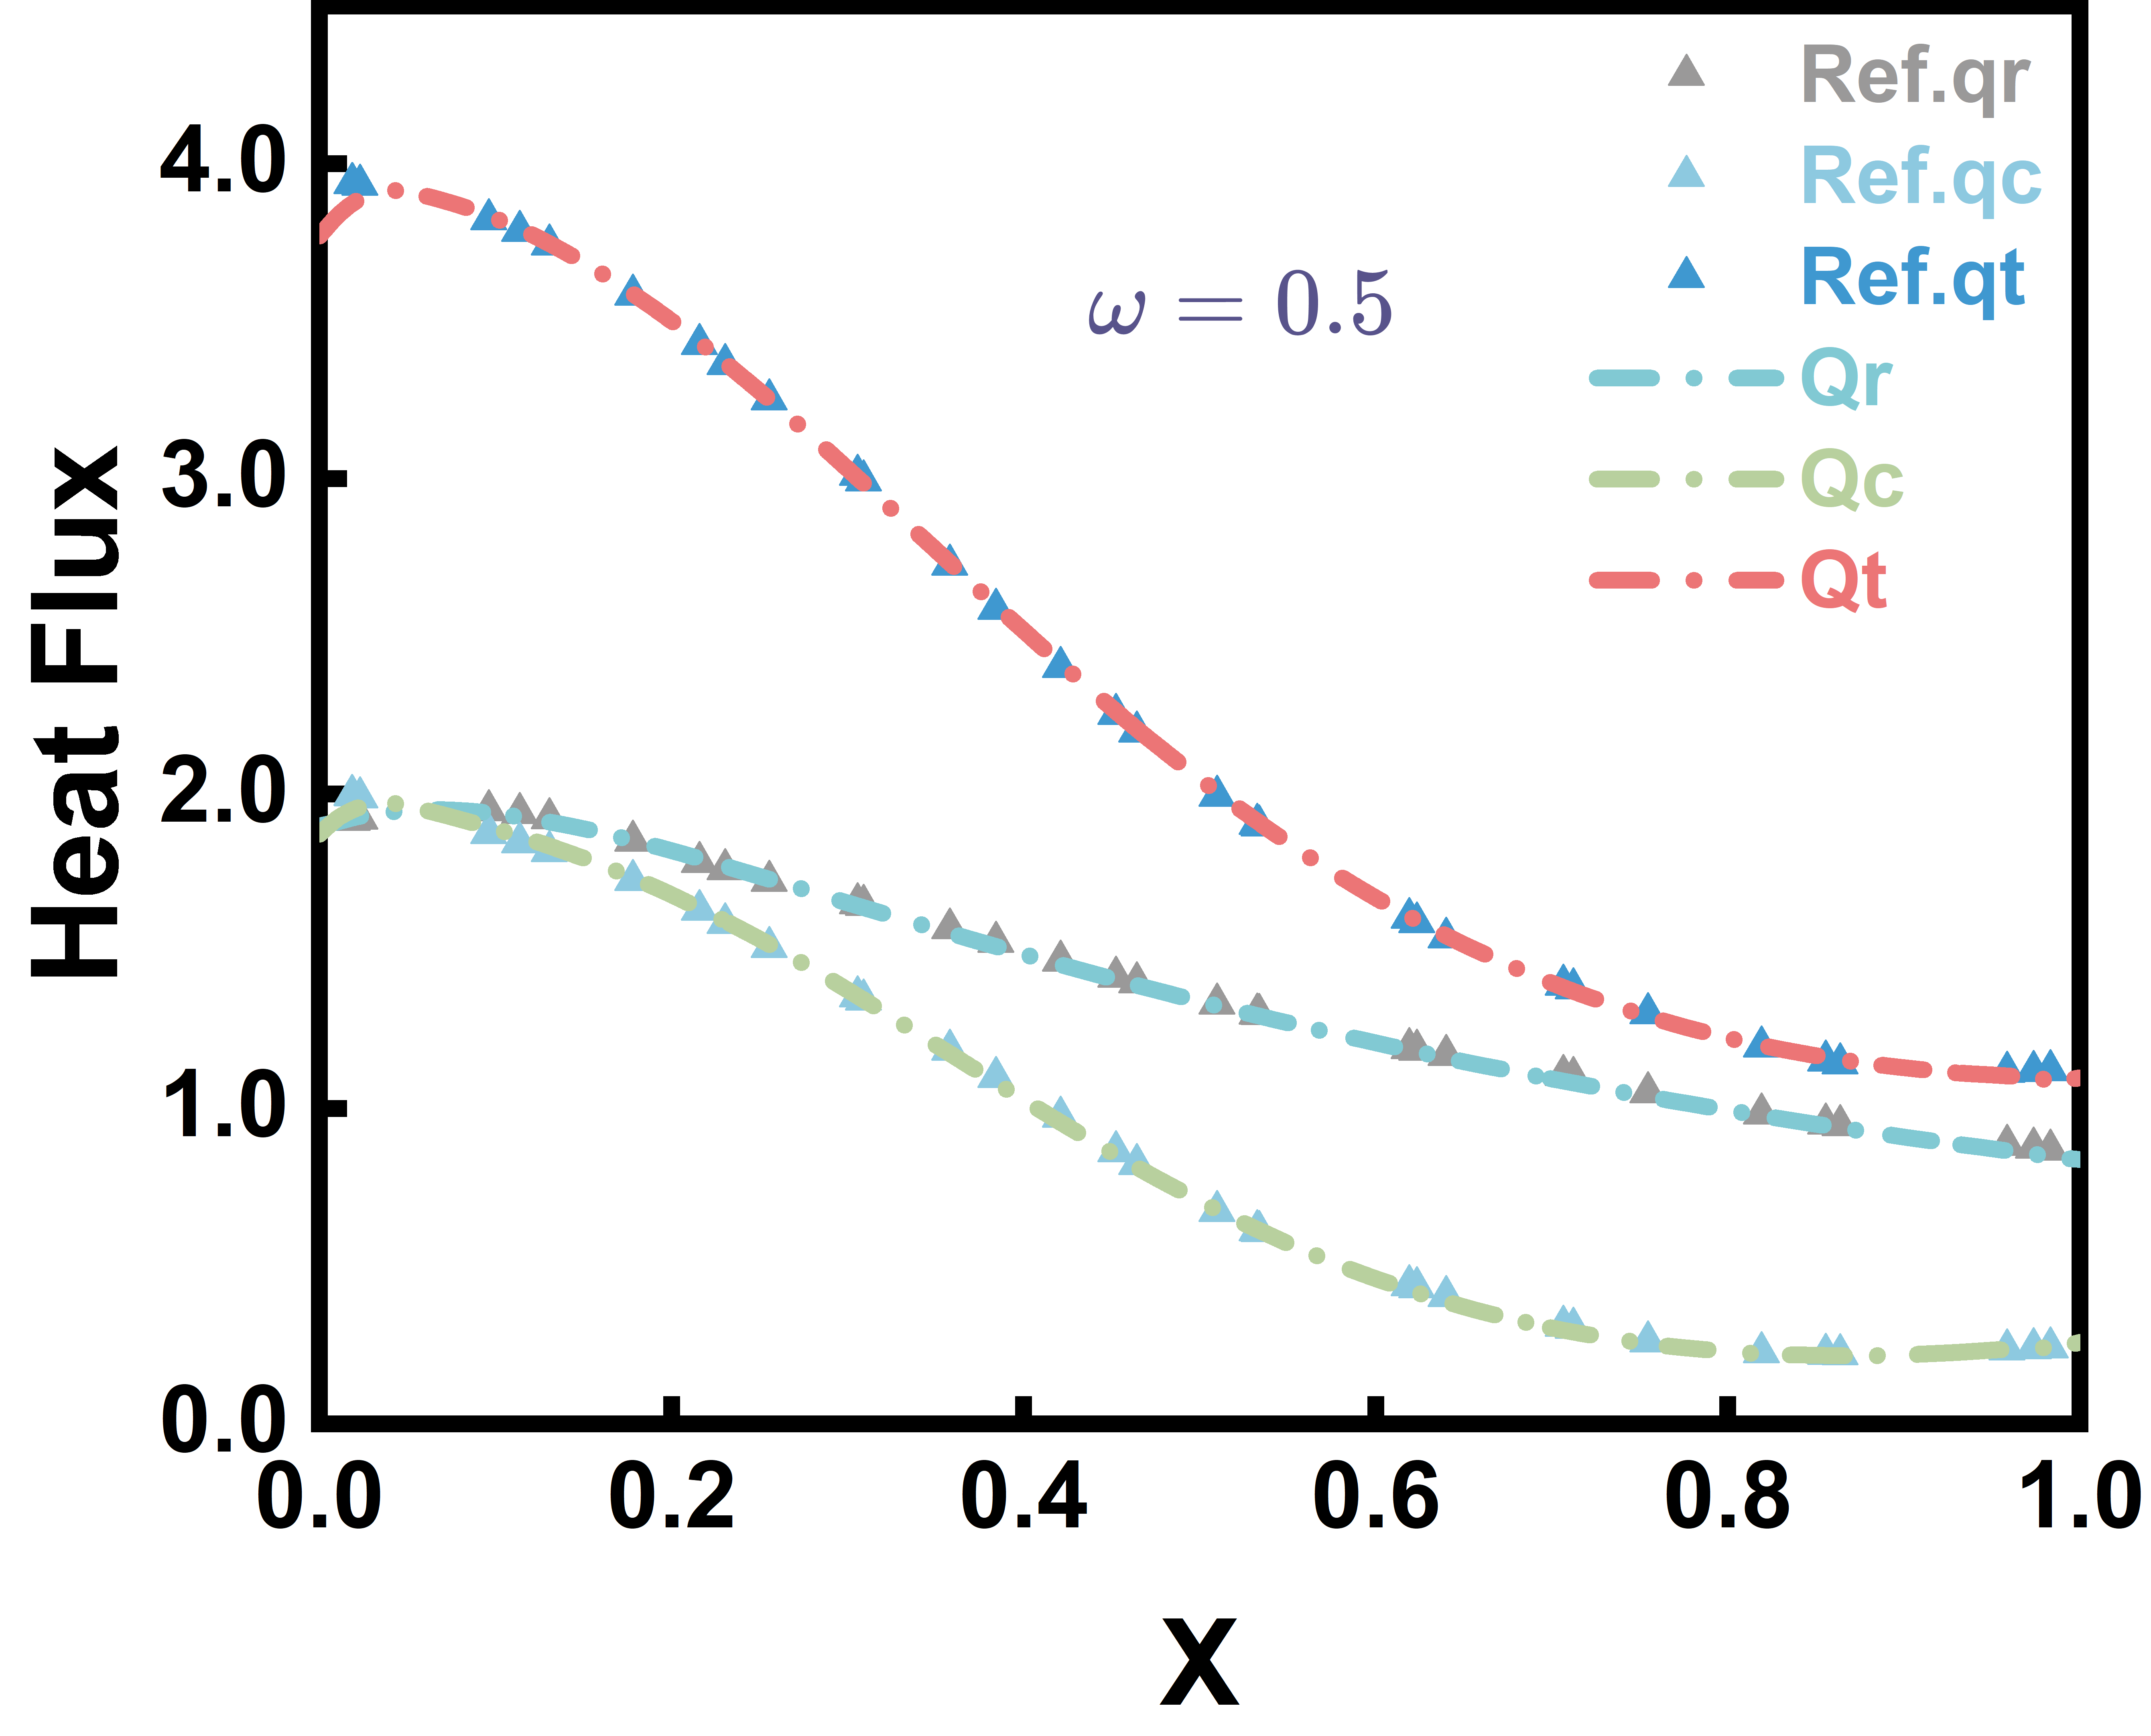
\includegraphics[width=\textwidth]{4B.png}
\caption{}
\end{subfigure}
\hfill
\begin{subfigure}[b]{\figwidth}
\centering
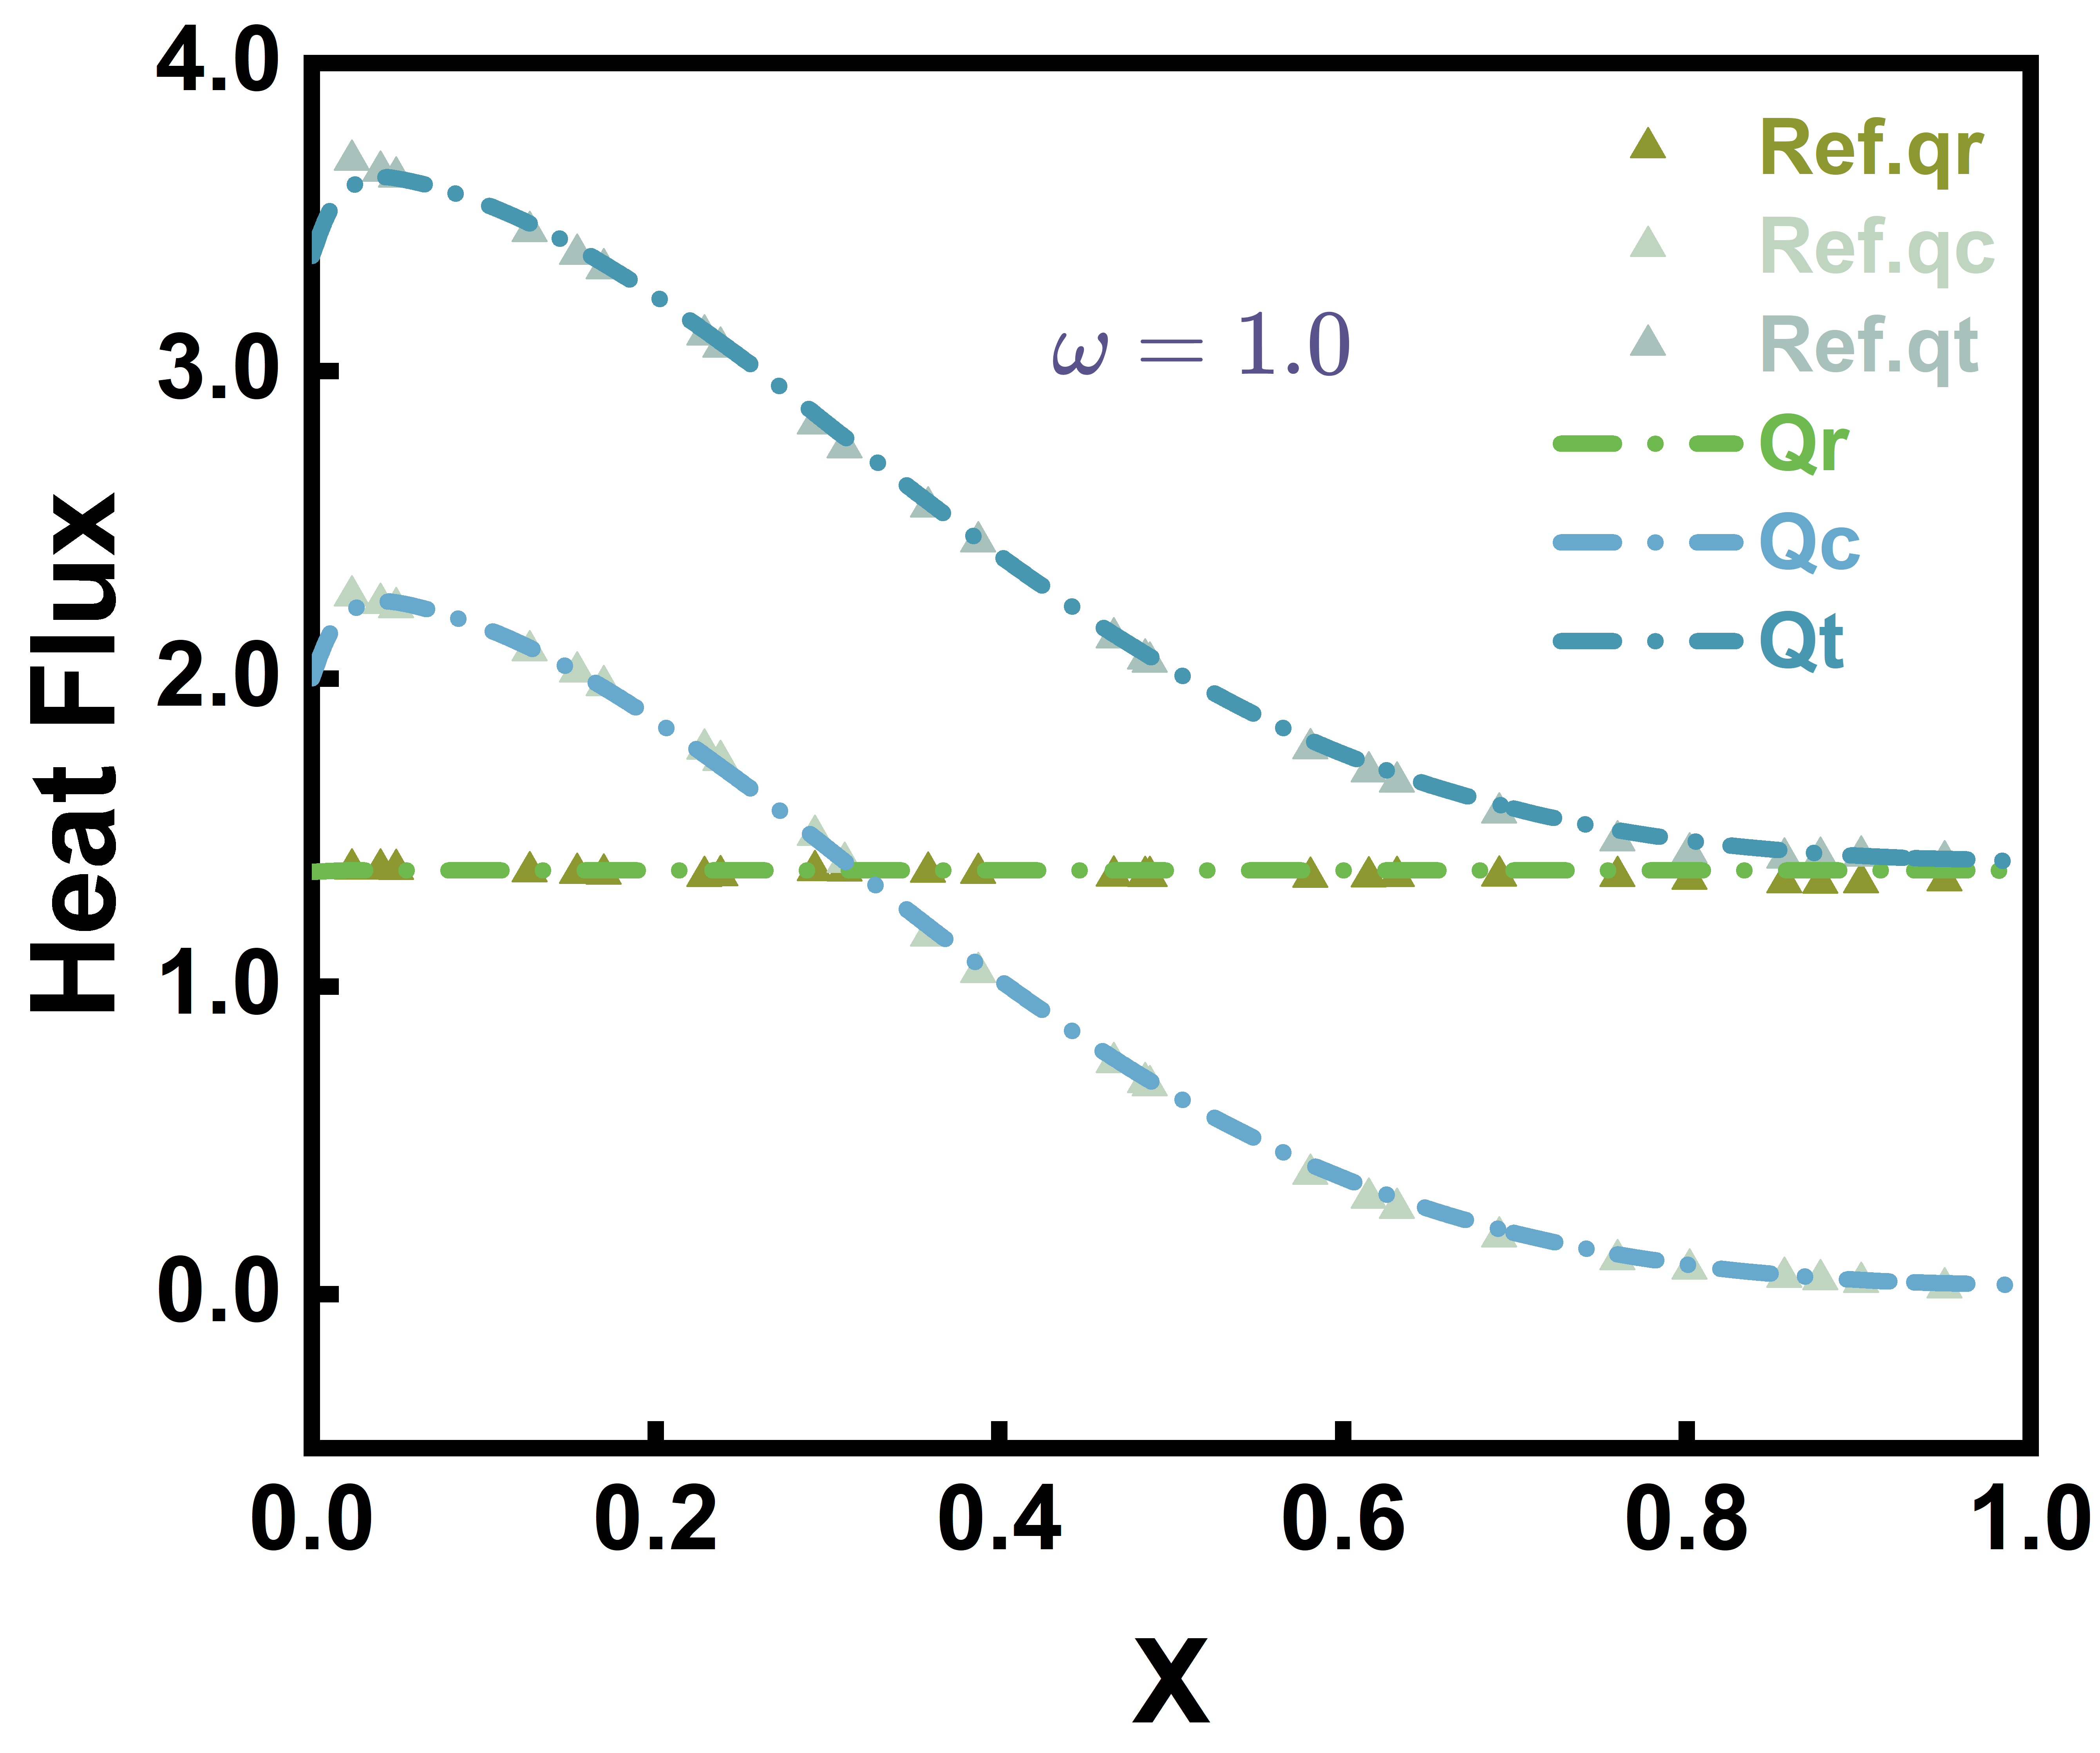
\includegraphics[width=\textwidth]{4C.png}
\caption{}
\end{subfigure}
\caption{Conductive, radiative, and total heat-flux profiles in the one-dimensional participating slab. The profiles are evaluated at $\zeta=0.005$ with $N=0.10$ , $T_E=0.1$. The scattering albedo is (a) $\omega=0$, (b) $\omega=0.5$,(c) $\omega=1.0$.}
\label{fig4}
\end{figure}

\subsection{2D cases}
\label{subsec:2d_cases}

The two-dimensional domain was a square medium of side length $L$, represented by $0\leq X,Y\leq1$. The square was initially at a uniform temperature $T_0$. At $t\geq0$, the south wall was raised to $T_S$ and held constant. The north, west, and east walls remained at $T_0$. All properties were constant, and the optical thickness was $1.0$ in both coordinate directions.

A uniform $41\times41$ mesh was used after further refinement produced negligible changes in the centreline temperature. The number of azimuthal control volumes was varied to assess angular sensitivity along the vertical centreline. Steady-state temperatures at $Y=0.3$, $0.5$, and $0.7$ were compared with the original benchmark matrix reproduced by Sun and Zhang~\cite{Sun2016} from Wu and Ou~\cite{WuOu1994}, Yuen and Takara~\cite{YuenTakara1988}, and Mondal and Mishra~\cite{MondalMishra2007}. For each value of $N$, the LBM--FVM solution reported by Sun and Zhang is included as a separate reference row, followed by the present DUGKS result. The comparison used $\tau_L=1.0$, $\omega=0$, $T_0=0.5$, and $N=1.0$, $0.1$, and $0.01$. Subsequent tests varied scattering albedo and the conduction--radiation parameter along the same centreline.

\begin{table}[H]
\centering
\scriptsize
\caption{Steady dimensionless temperature $T/T_S$ on the vertical centreline of the two-dimensional square enclosure at $\tau_L=1.0$, $\omega=0$, and $T_0=0.5$. The original comparison data and the LBM--FVM solutions are taken from Sun and Zhang~\cite{Sun2016}; for each $N$, the present DUGKS results obtained using $N_\theta=8$ and $N_\phi=16$ are listed immediately after the LBM--FVM reference.}
\label{tab:square_validation}
\resizebox{\textwidth}{!}{%
\begin{tabular}{@{}c l ccc@{}}
\toprule
$N$ & Investigator/method & $Y=0.30$ & $Y=0.50$ & $Y=0.70$ \\
\midrule
\multirow{5}{*}{1.00}
& Wu and Ou~\cite{WuOu1994}                    & 0.733 & 0.630 & 0.560 \\
& Yuen and Takara~\cite{YuenTakara1988}         & 0.737 & 0.630 & 0.560 \\
& Mondal and Mishra~\cite{MondalMishra2007}     & 0.738 & 0.631 & 0.565 \\
& LBM--FVM (Sun and Zhang)~\cite{Sun2016}       & 0.734 & 0.630 & 0.565 \\
& Present DUGKS                                  & 0.738 & 0.630 & 0.563 \\
\midrule
\multirow{5}{*}{0.10}
& Wu and Ou~\cite{WuOu1994}                    & 0.760 & 0.663 & 0.590 \\
& Yuen and Takara~\cite{YuenTakara1988}         & 0.763 & 0.661 & 0.589 \\
& Mondal and Mishra~\cite{MondalMishra2007}     & 0.761 & 0.667 & 0.598 \\
& LBM--FVM (Sun and Zhang)~\cite{Sun2016}       & 0.757 & 0.664 & 0.596 \\
& Present DUGKS                                  & 0.760 & 0.663 & 0.593 \\
\midrule
\multirow{5}{*}{0.01}
& Wu and Ou~\cite{WuOu1994}                    & 0.791 & 0.725 & 0.663 \\
& Yuen and Takara~\cite{YuenTakara1988}         & 0.807 & 0.726 & 0.653 \\
& Mondal and Mishra~\cite{MondalMishra2007}     & 0.777 & 0.722 & 0.672 \\
& LBM--FVM (Sun and Zhang)~\cite{Sun2016}       & 0.786 & 0.725 & 0.668 \\
& Present DUGKS                                  & 0.788 & 0.724 & 0.665 \\
\bottomrule
\end{tabular}%
}
\end{table}

Table~\ref{tab:square_validation} extends the verification beyond the one-dimensional slab. The present DUGKS results follow the reference centreline temperatures over the conduction-dominated, intermediate, and radiation-dominated values of $N$; the maximum absolute difference from the LBM--FVM results of Sun and Zhang~\cite{Sun2016} is $4.0\times10^{-3}$. Temperature and radiation are evaluated on the same control-volume grid in all present calculations.

\begin{figure}[H]
\centering
\begin{subfigure}[b]{\figwidth}
\centering
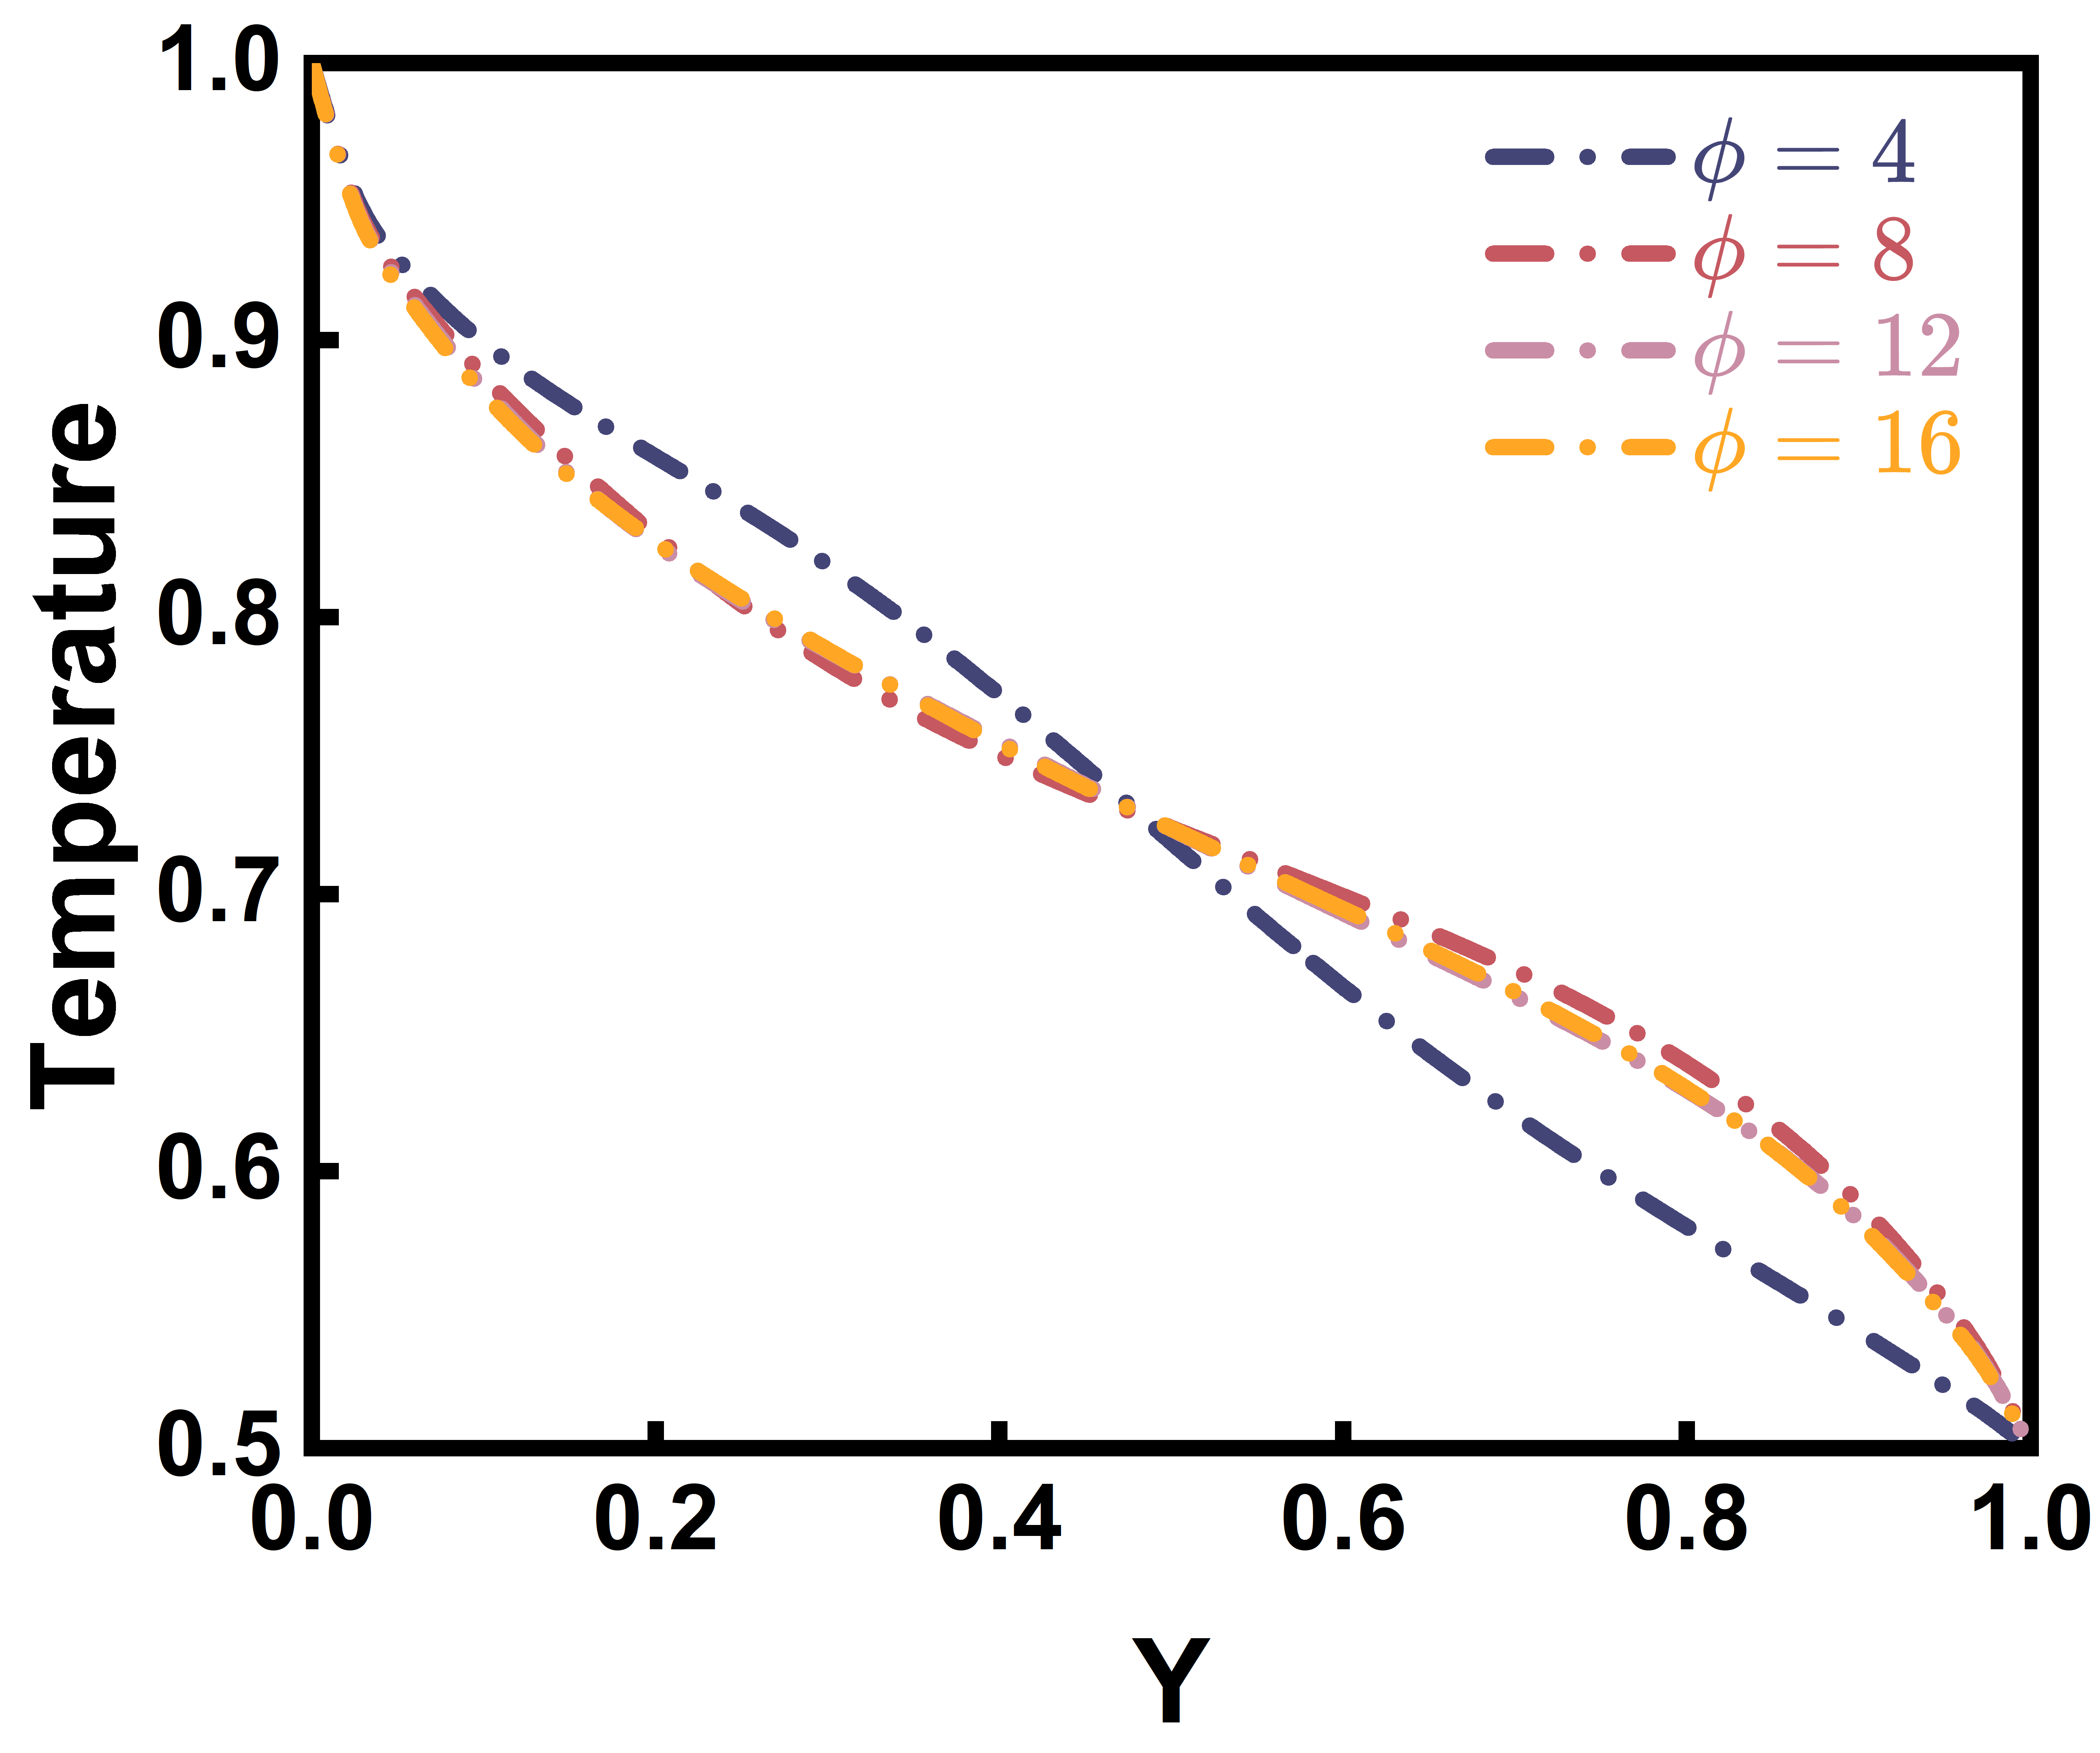
\includegraphics[width=\textwidth]{5A.png}
\caption{}
\end{subfigure}
\hfill
\begin{subfigure}[b]{\figwidth}
\centering
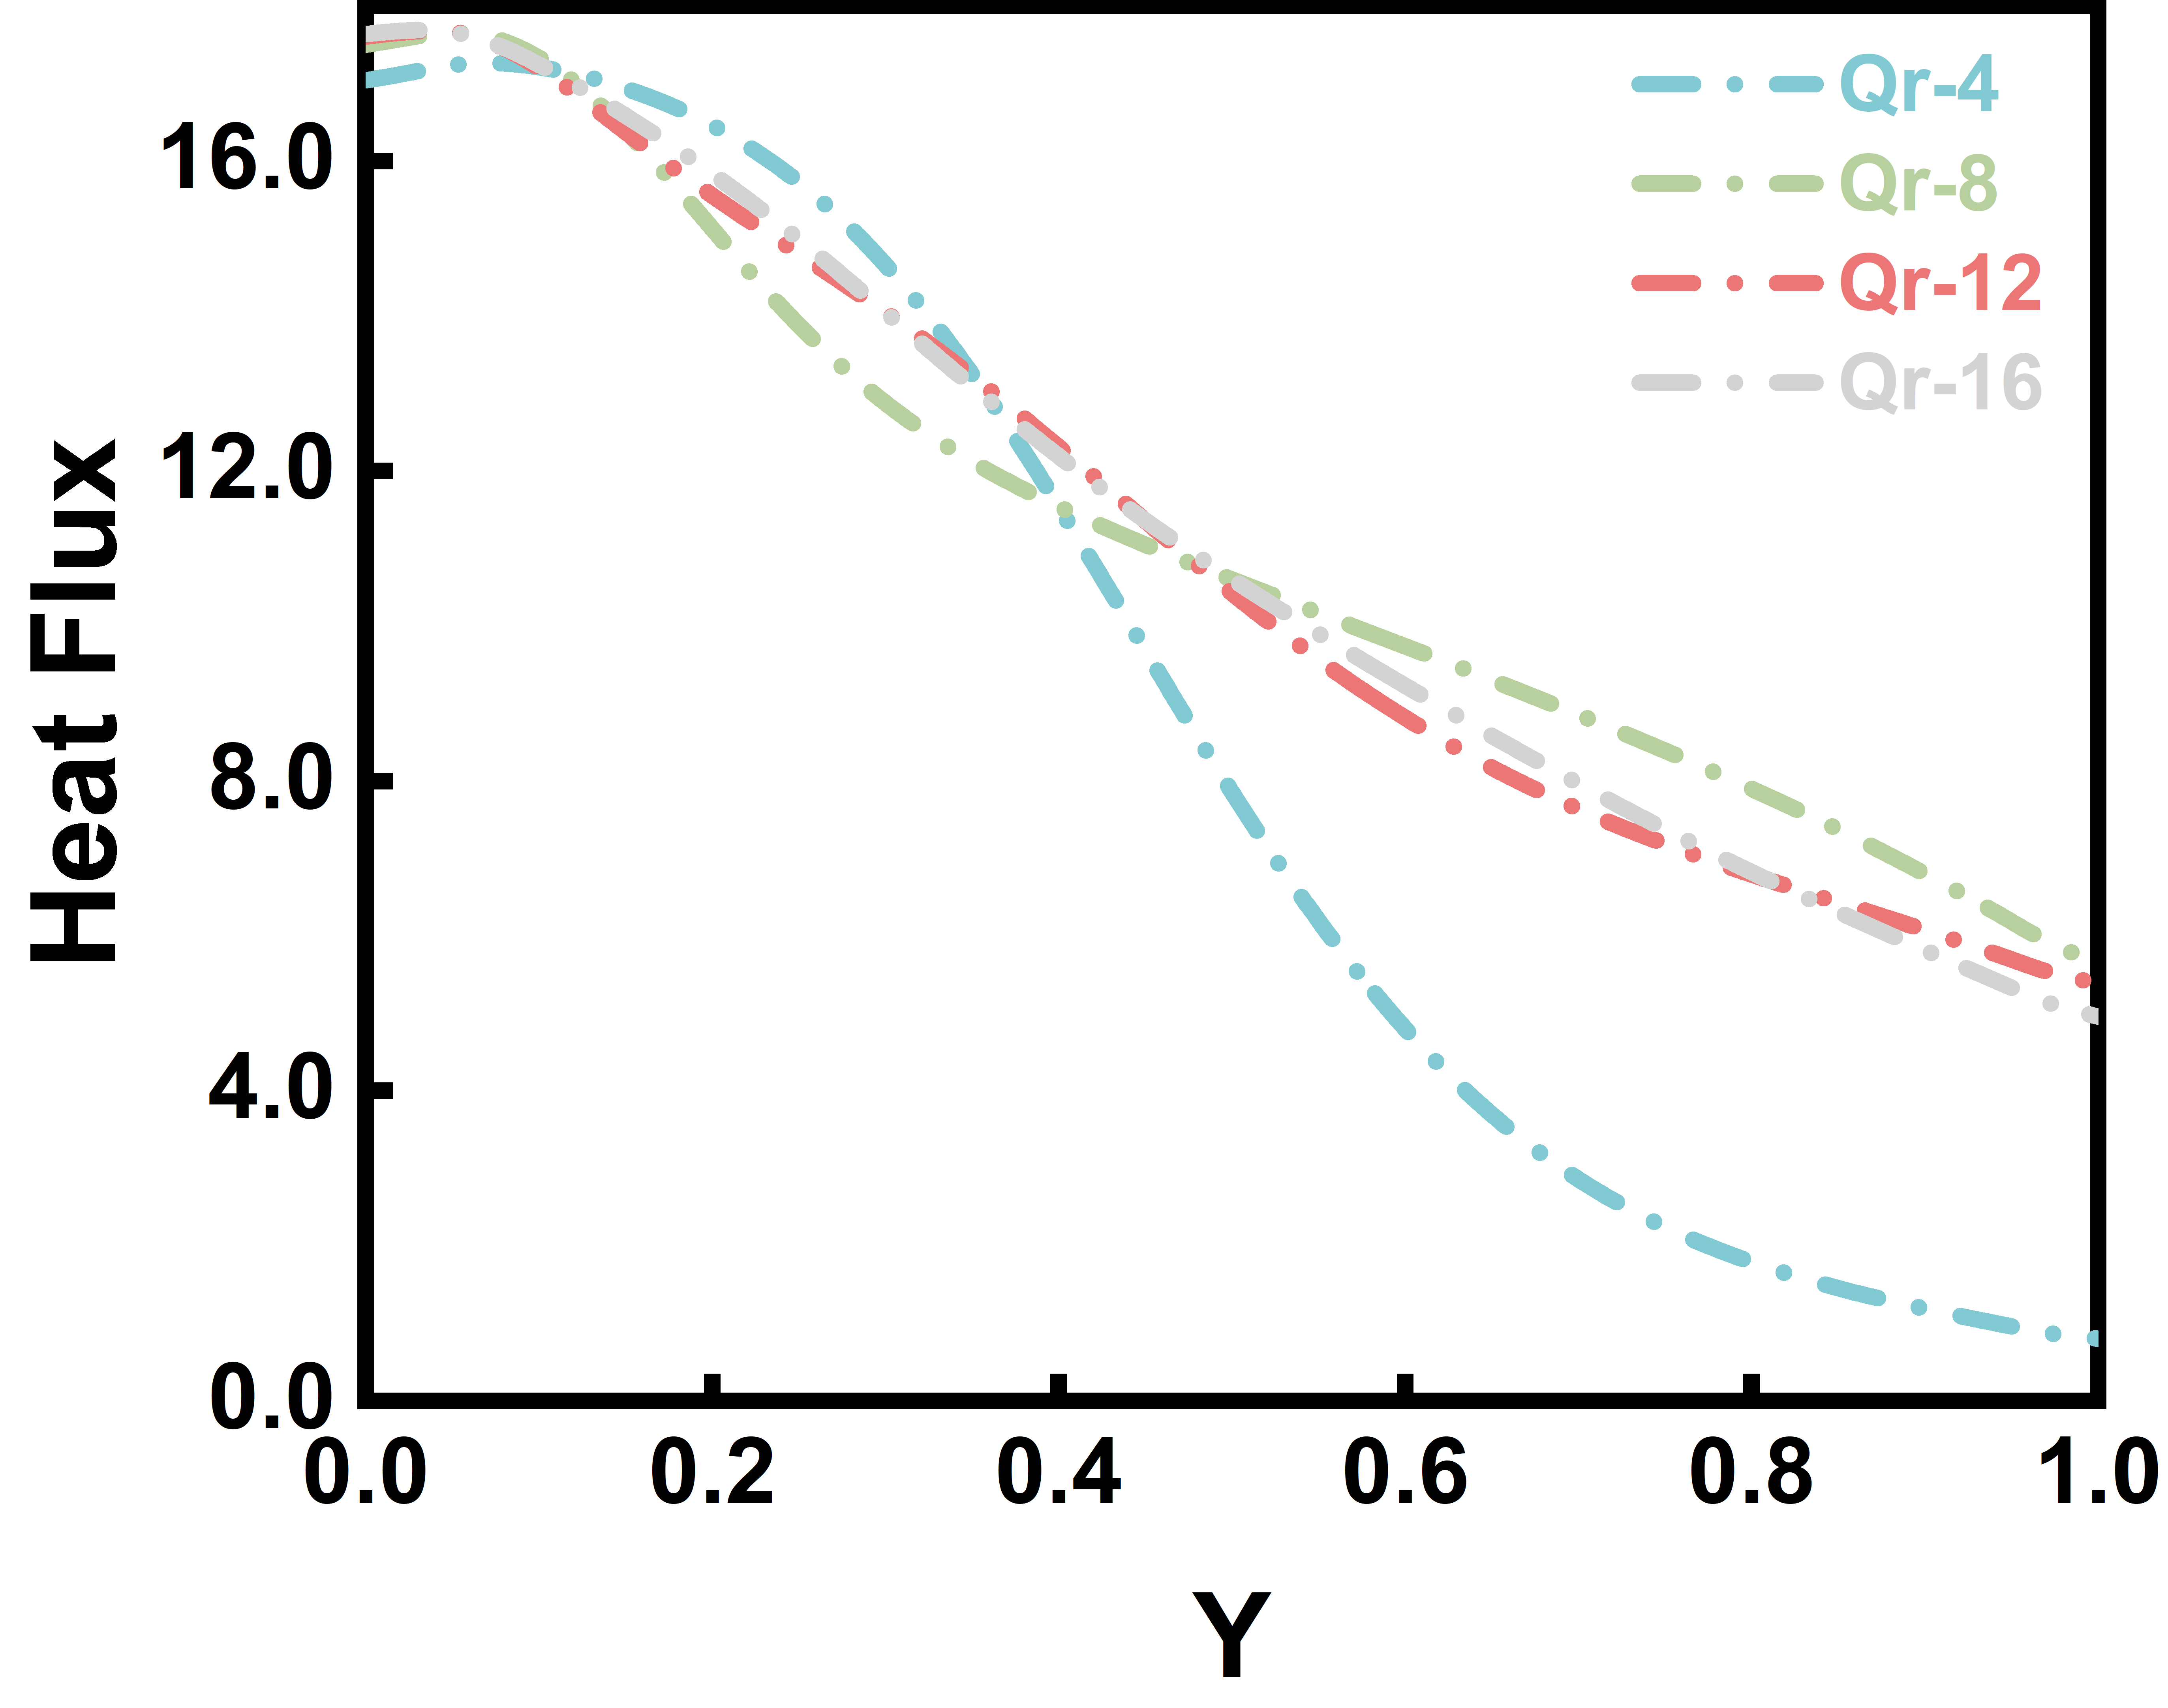
\includegraphics[width=\textwidth]{5B.png}
\caption{}
\end{subfigure}
\hfill
\begin{subfigure}[b]{\figwidth}
\centering
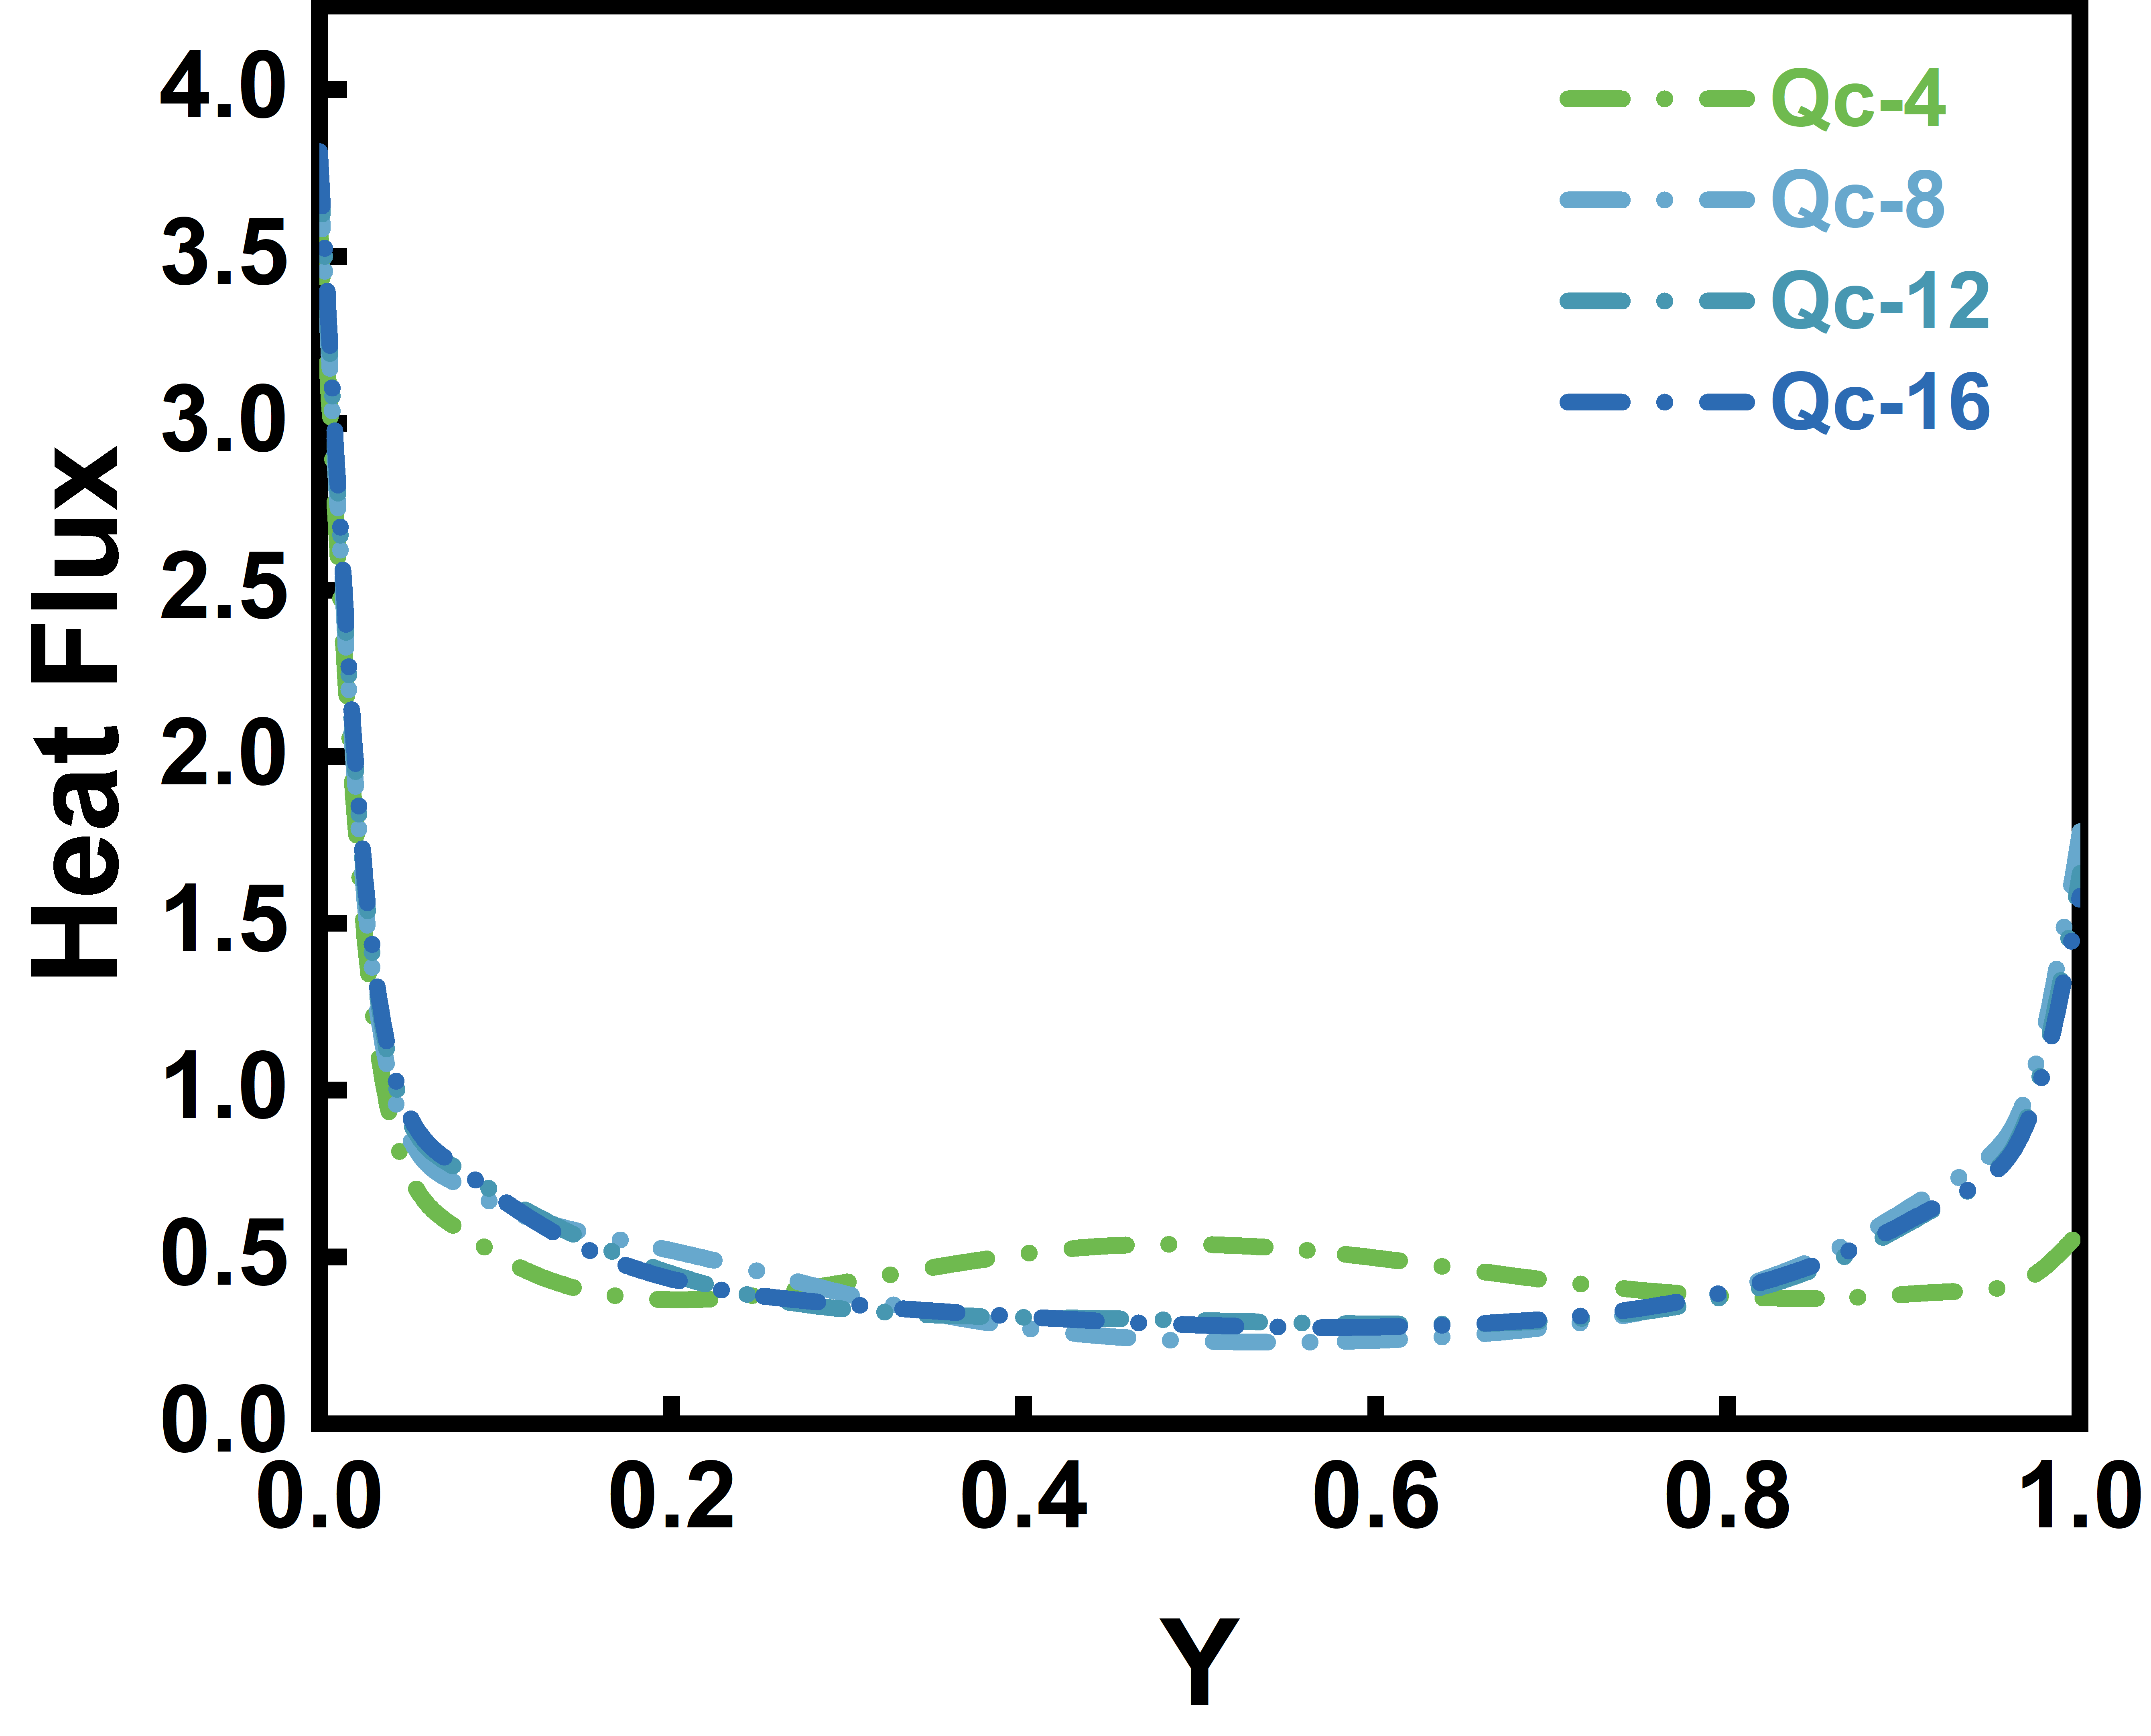
\includegraphics[width=\textwidth]{5C.png}
\caption{}
\end{subfigure}
\caption{Sensitivity of steady-state centreline profiles to azimuthal angular resolution in the two-dimensional square enclosure. The panels show (a) temperature, (b) radiative heat flux $q_r$,(c) conductive heat flux $q_c$. Calculations use $N=0.01$, $\omega=0$, $N_\theta=8$, and $N_\phi=4$, $8$, $12$, $16$.}
\label{fig5}
\end{figure}

Figure~\ref{fig5} compares centreline profiles for $N_\phi=4$, $8$, $12$, and $16$ azimuthal control volumes. The temperature profile changed markedly from $N_\phi=4$ to $N_\phi=8$. Differences among $N_\phi=8$, $12$, and $16$ were smaller. The heat-flux profiles were more sensitive, with visible differences remaining between $N_\phi=8$ and the finer discretisations. All subsequent two-dimensional calculations therefore used $N_\phi=16$.

\begin{figure}[H]
\centering
\begin{subfigure}[b]{\figwidth}
\centering
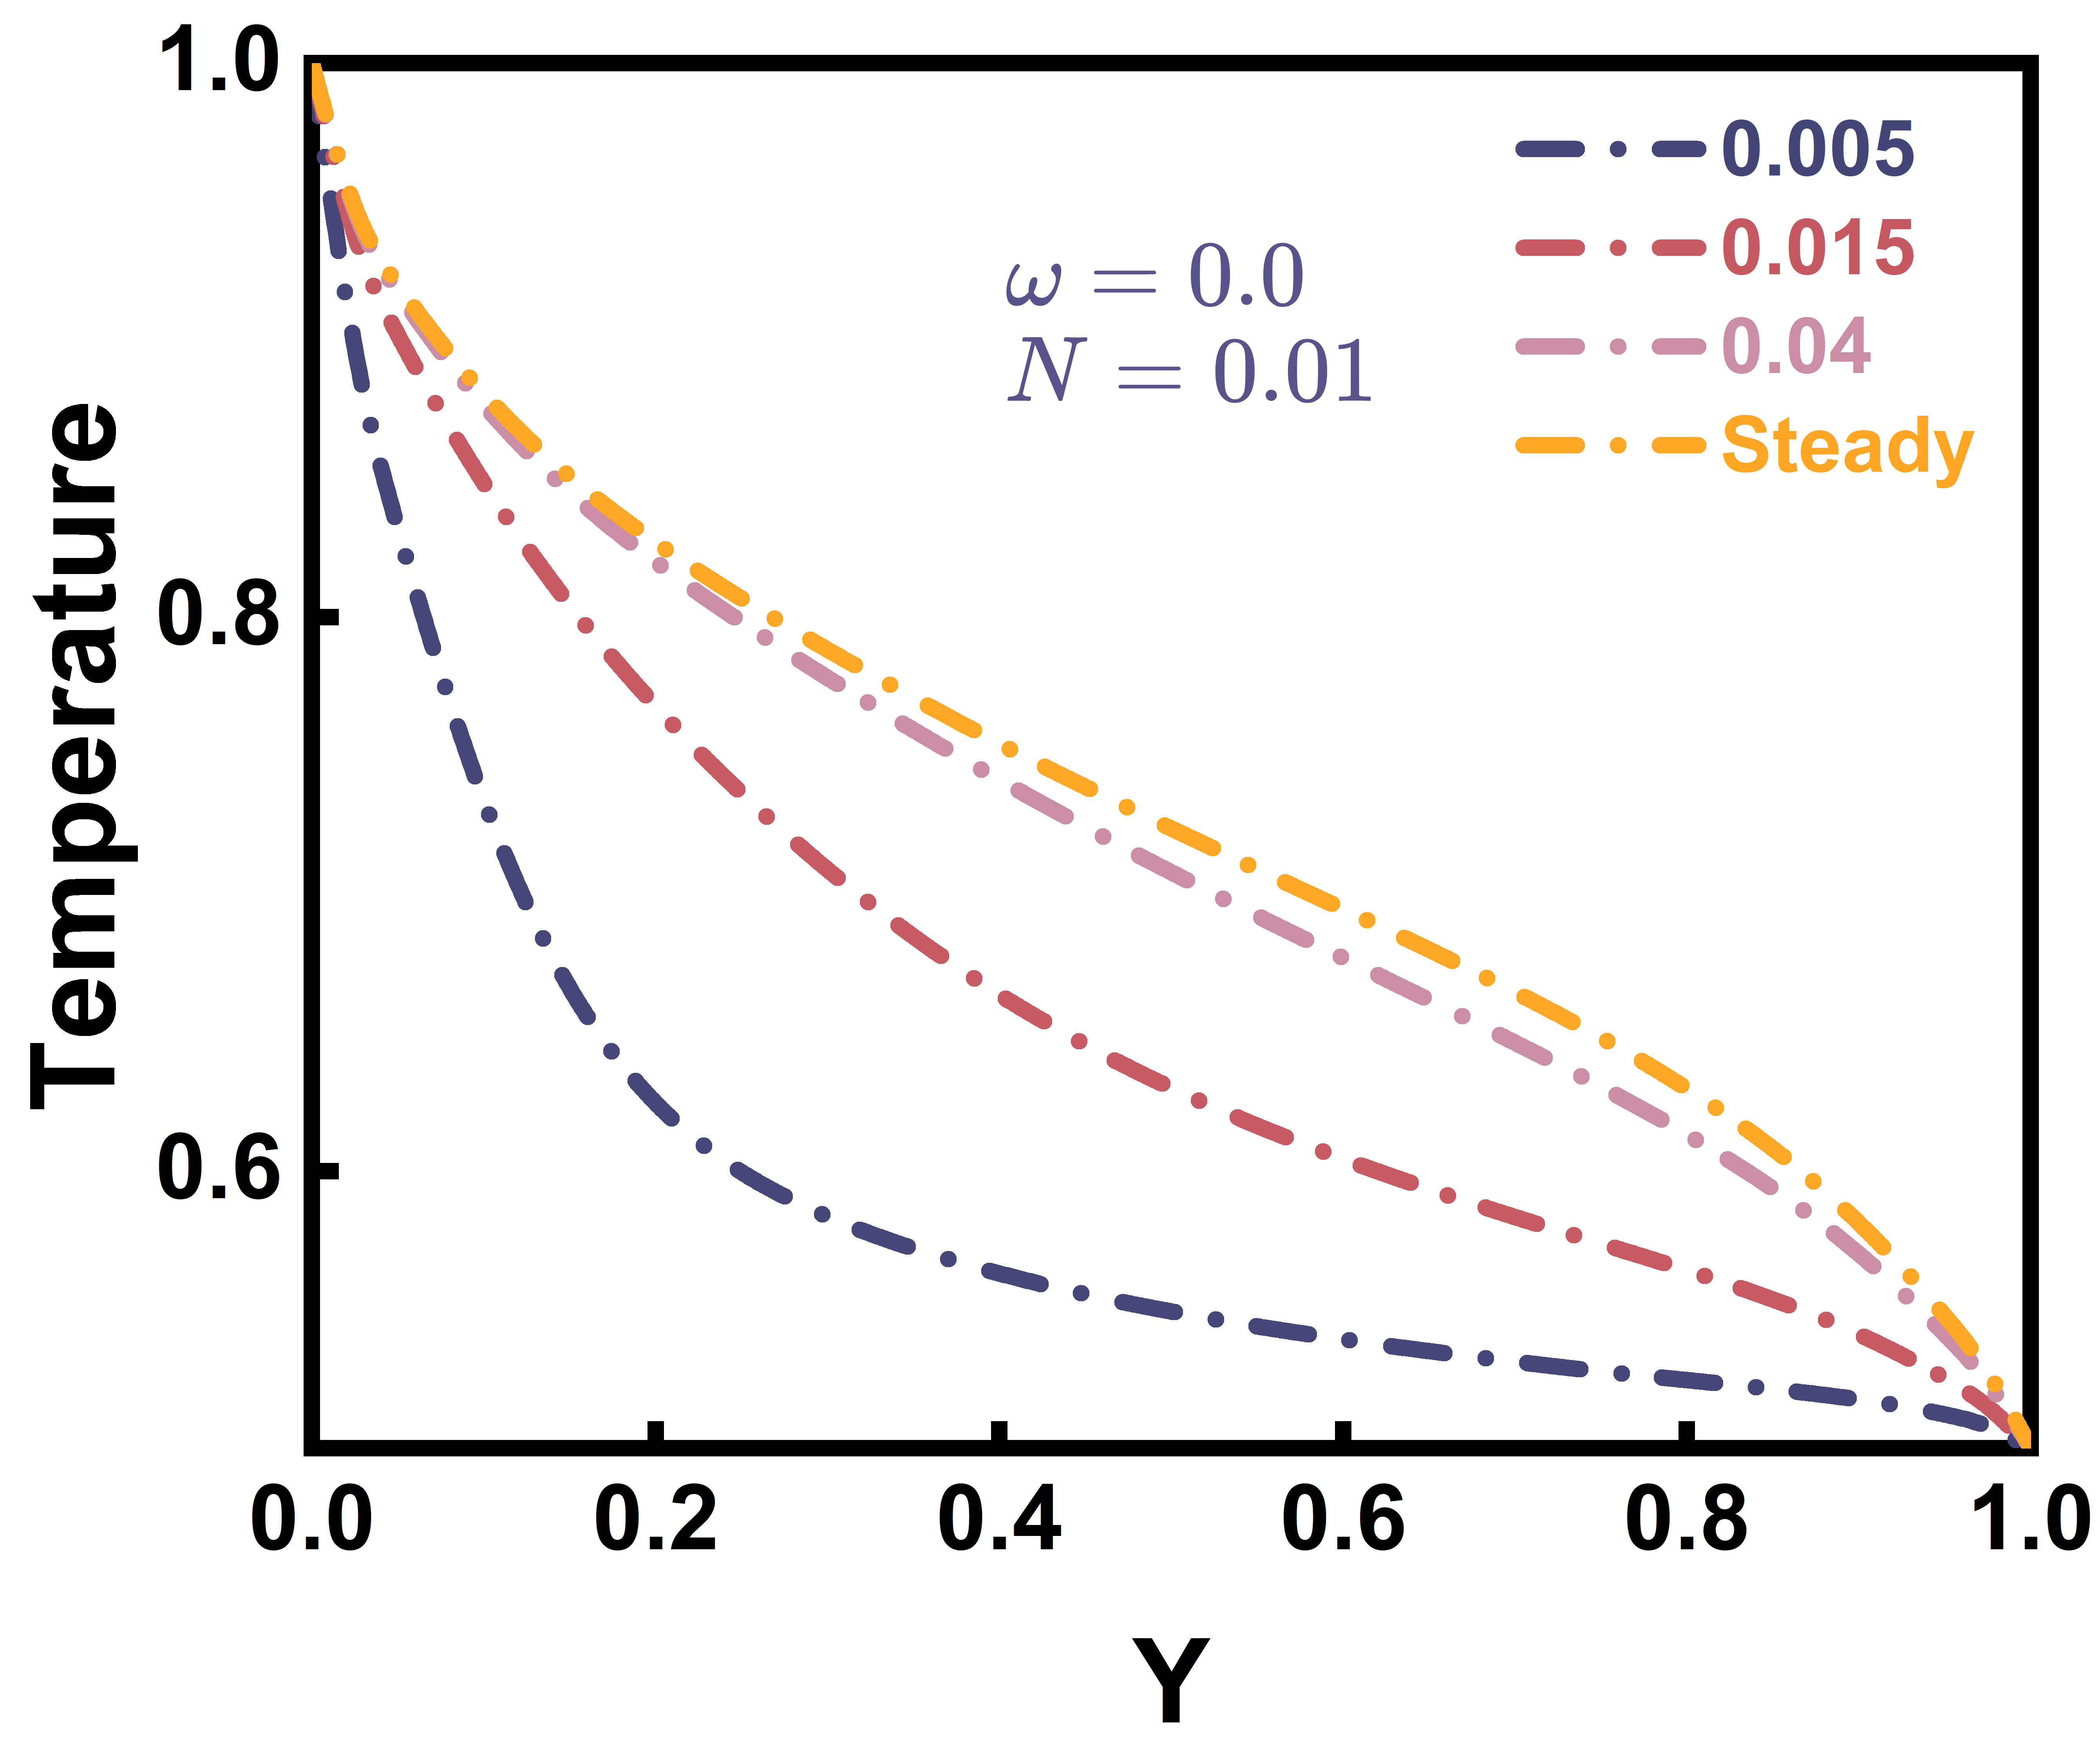
\includegraphics[width=\textwidth]{6A.png}
\caption{}
\end{subfigure}
\hfill
\begin{subfigure}[b]{\figwidth}
\centering
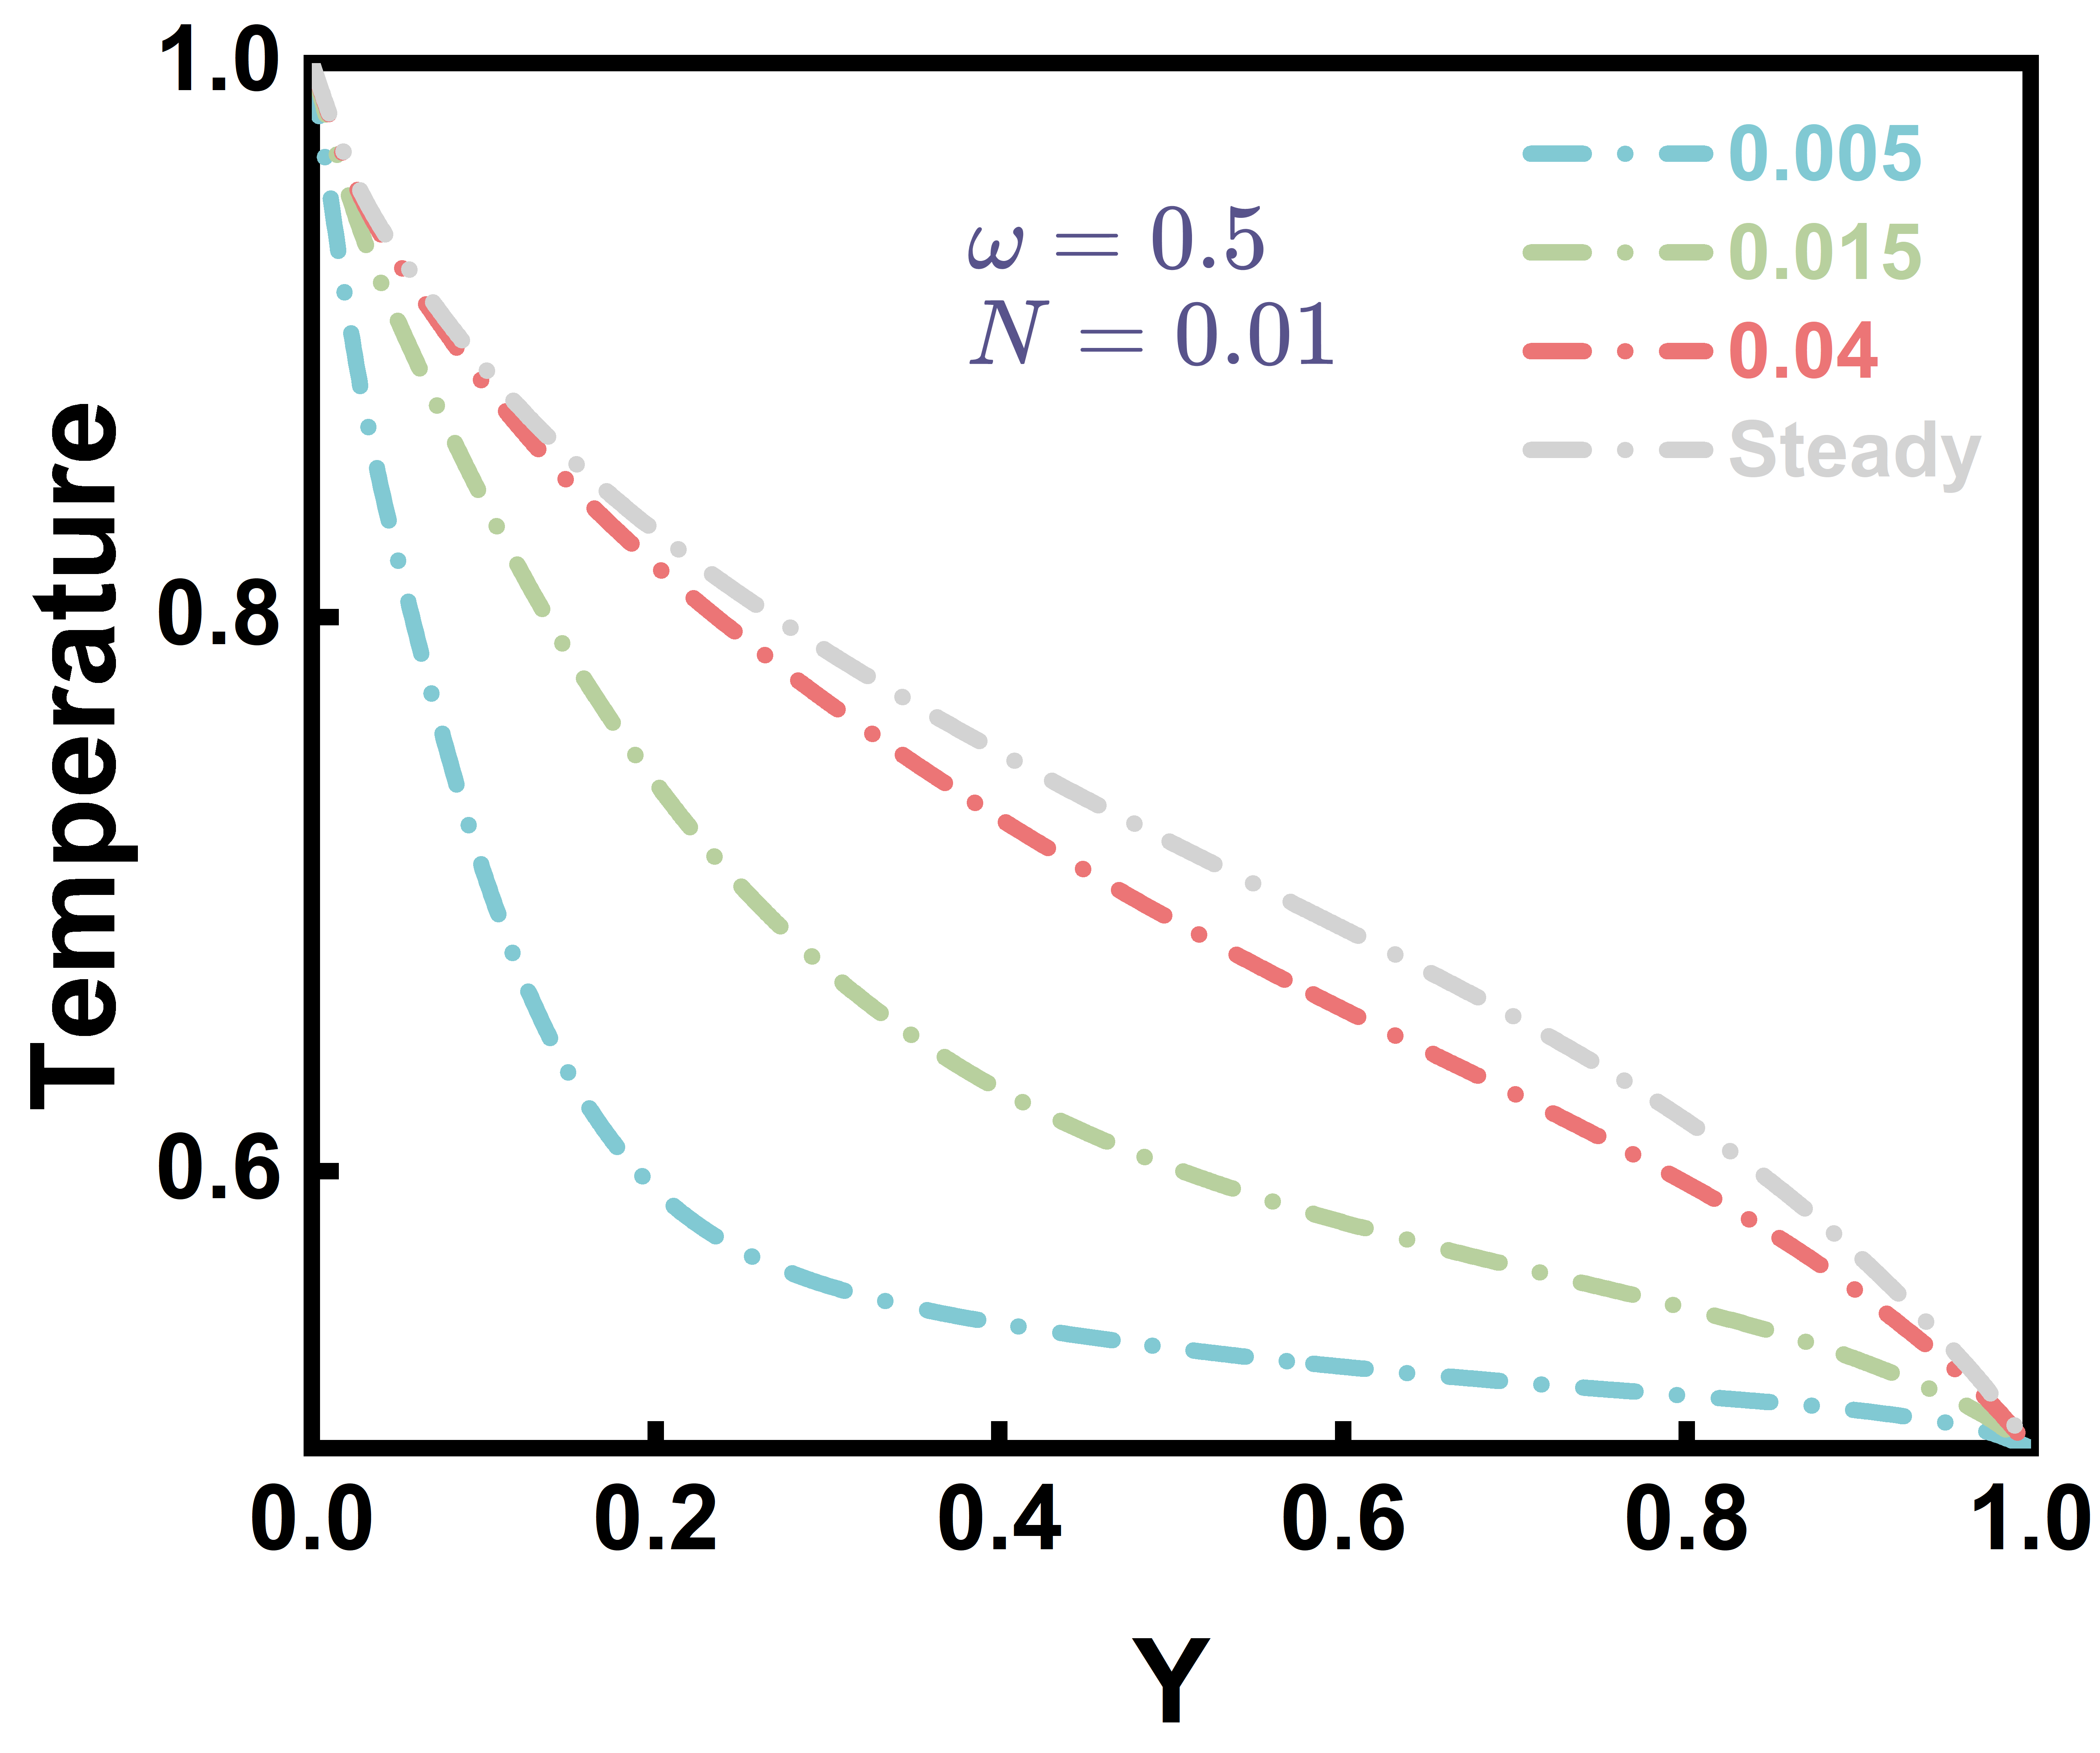
\includegraphics[width=\textwidth]{6B.png}
\caption{}
\end{subfigure}
\hfill
\begin{subfigure}[b]{\figwidth}
\centering
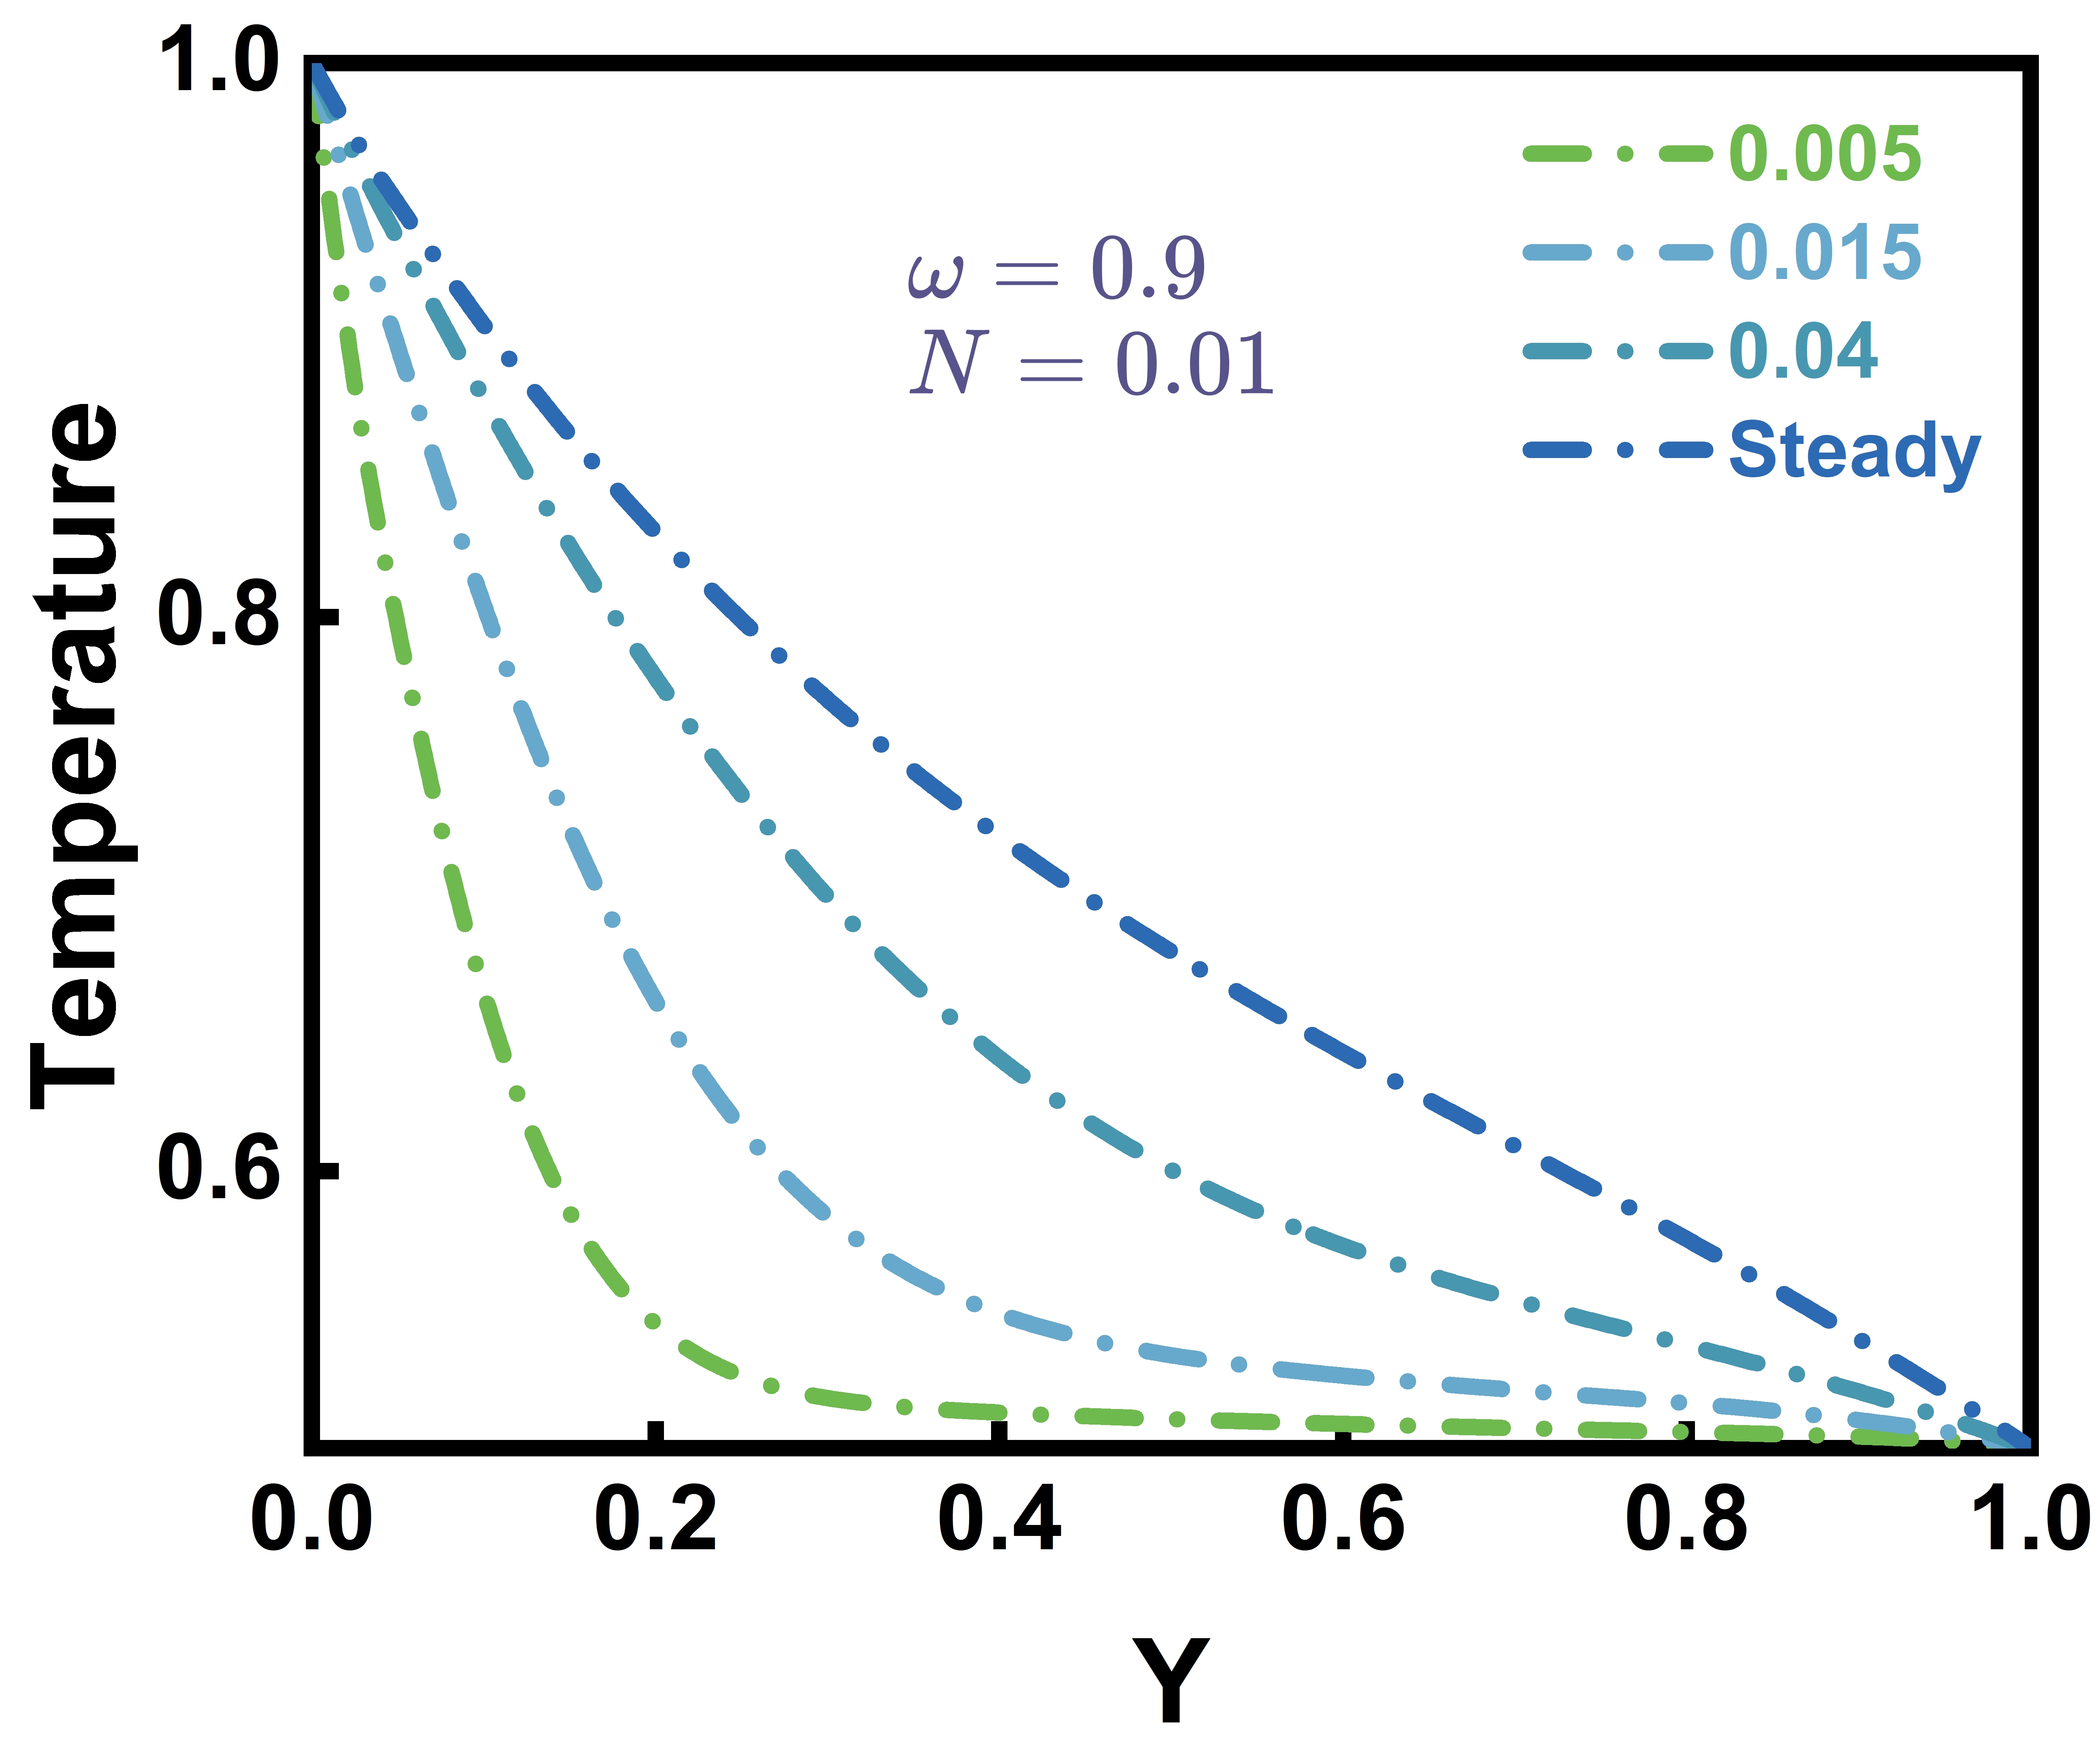
\includegraphics[width=\textwidth]{6C.png}
\caption{}
\end{subfigure}
\caption{Transient centreline temperature profiles in the two-dimensional square enclosure at $N=0.01$ ,$T_0=0.5$. The scattering albedo is (a) $\omega=0$, (b) $\omega=0.5$,(c) $\omega=0.9$.}
\label{fig6}
\end{figure}

Figure~\ref{fig6} shows transient centreline temperatures for different scattering albedos. Increasing $\omega$ lowered the temperature and increased the time required to approach steady state. The two-dimensional temperatures were lower than their one-dimensional counterparts under corresponding conditions. At lower $\omega$, the steady-state temperature gradient near the north wall was larger.

\begin{figure}[H]
\centering
\begin{subfigure}[b]{\figwidth}
\centering
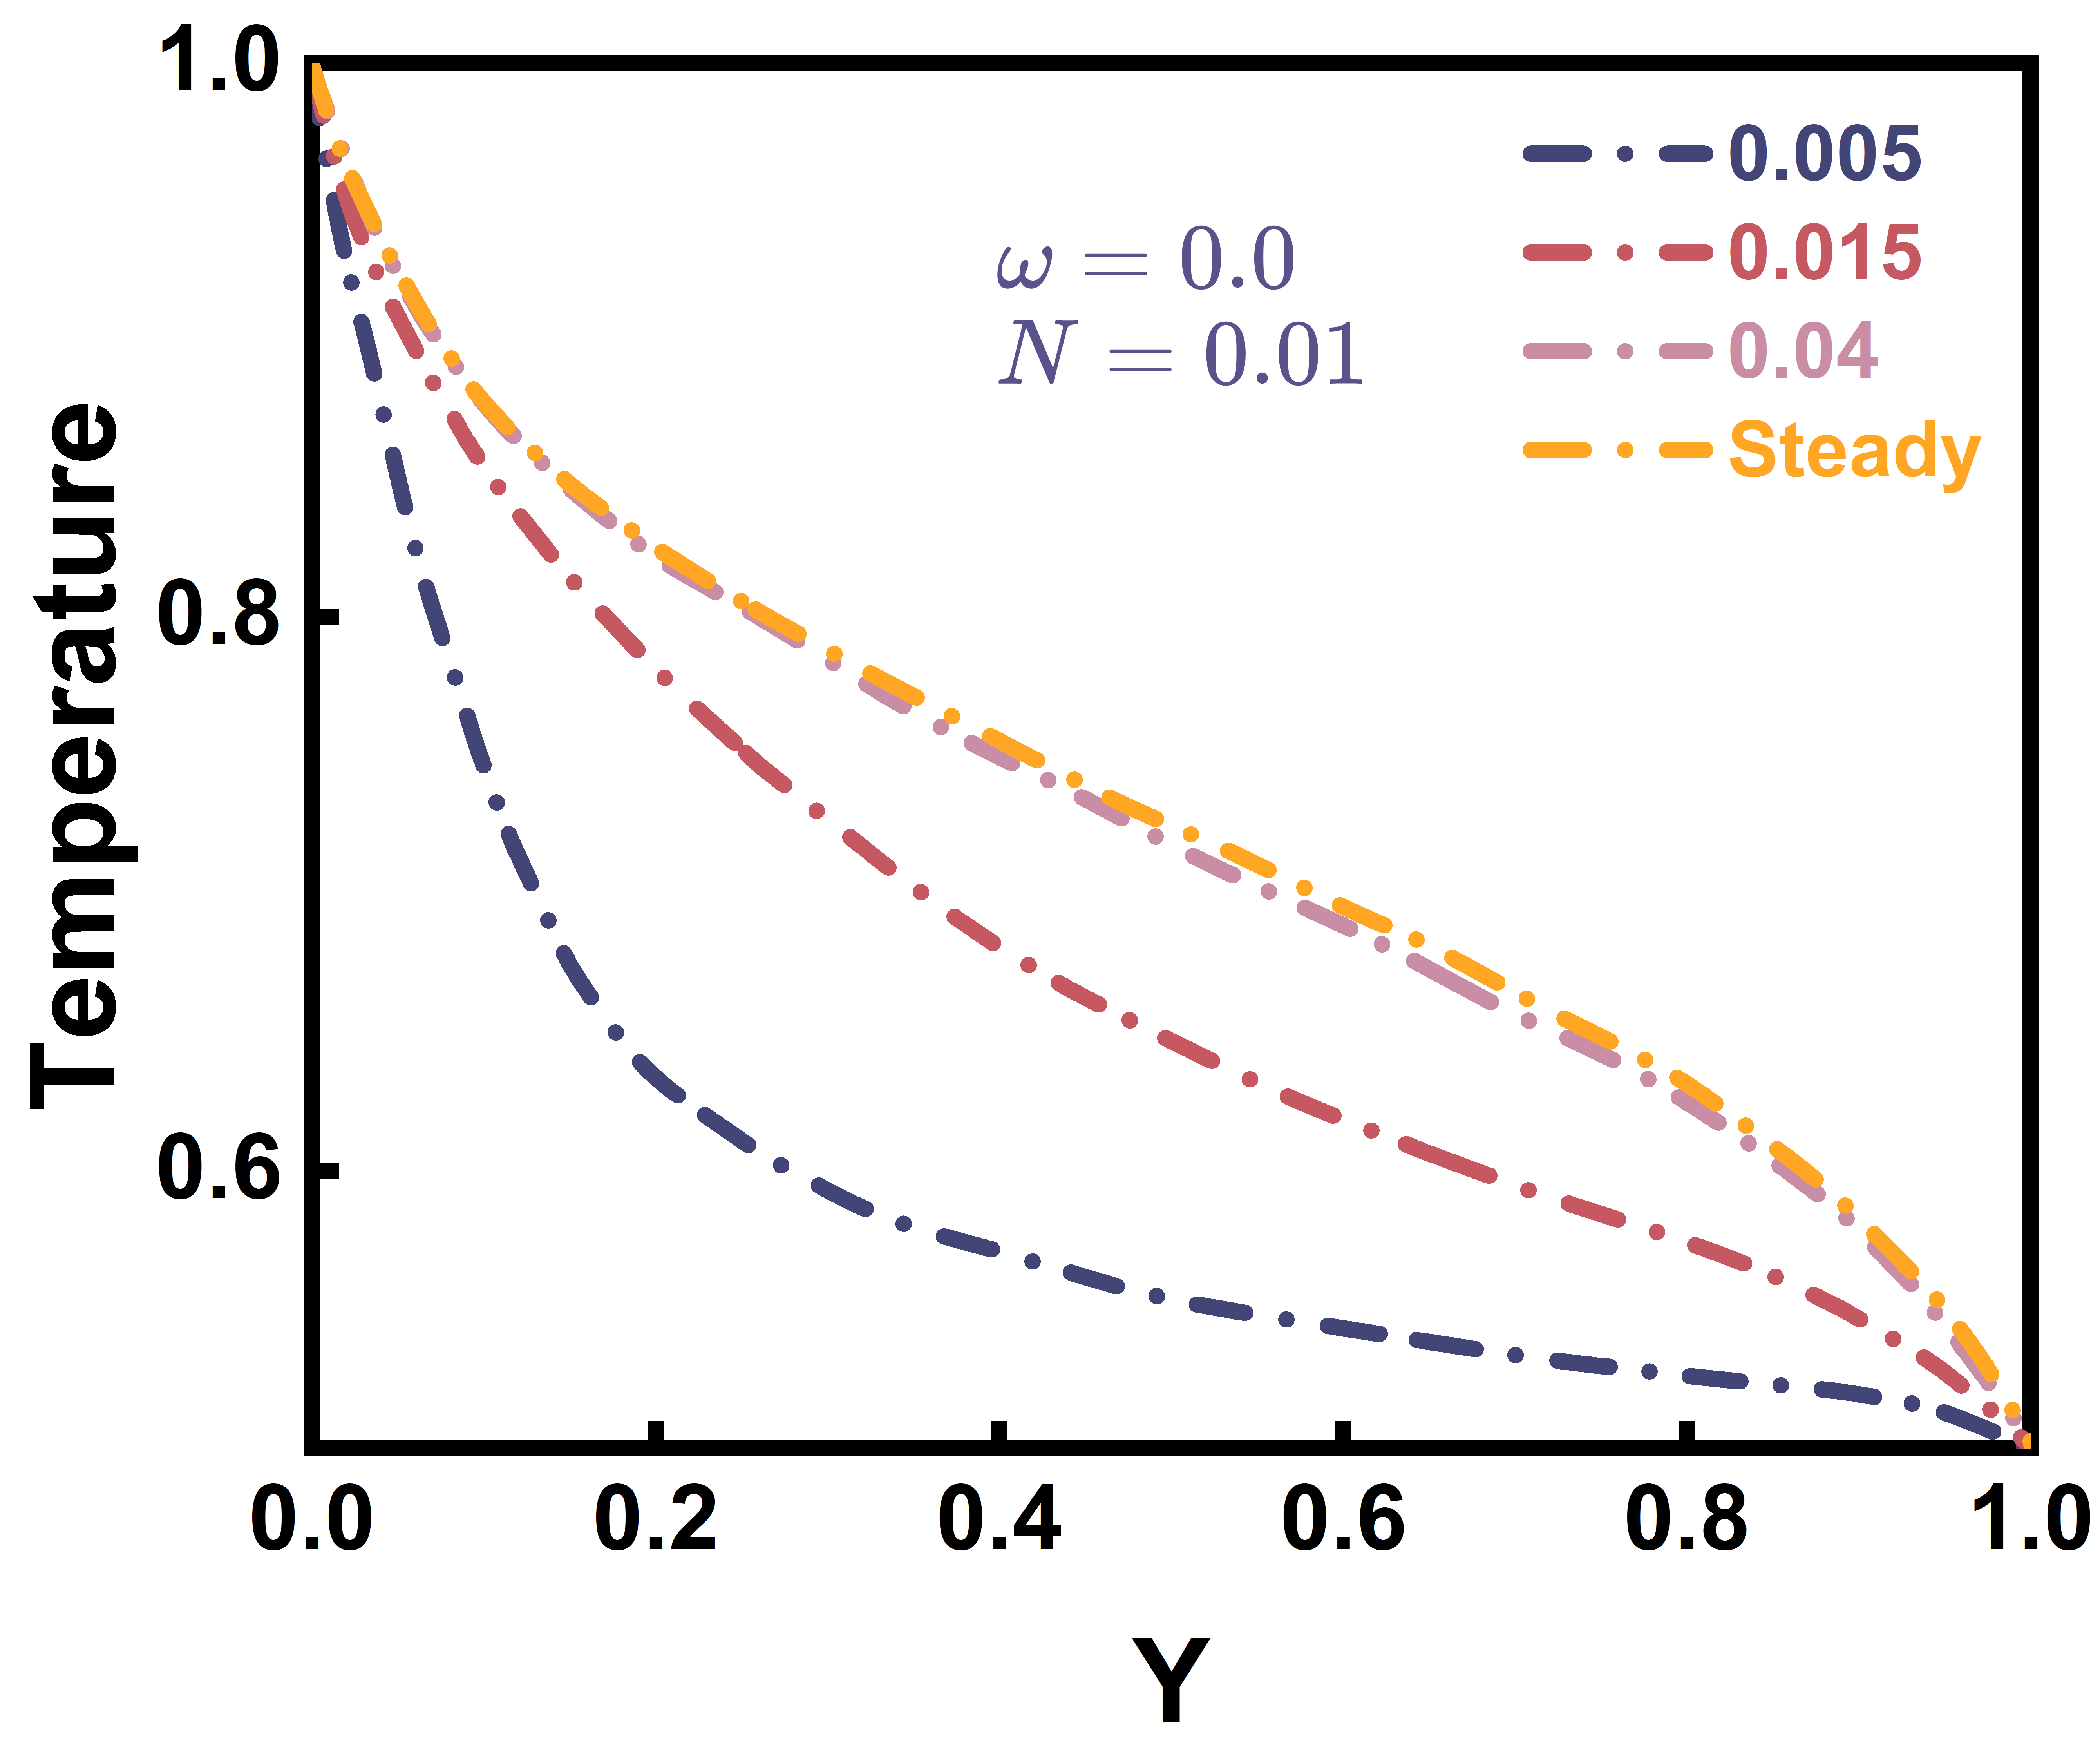
\includegraphics[width=\textwidth]{7A.png}
\caption{}
\end{subfigure}
\hfill
\begin{subfigure}[b]{\figwidth}
\centering
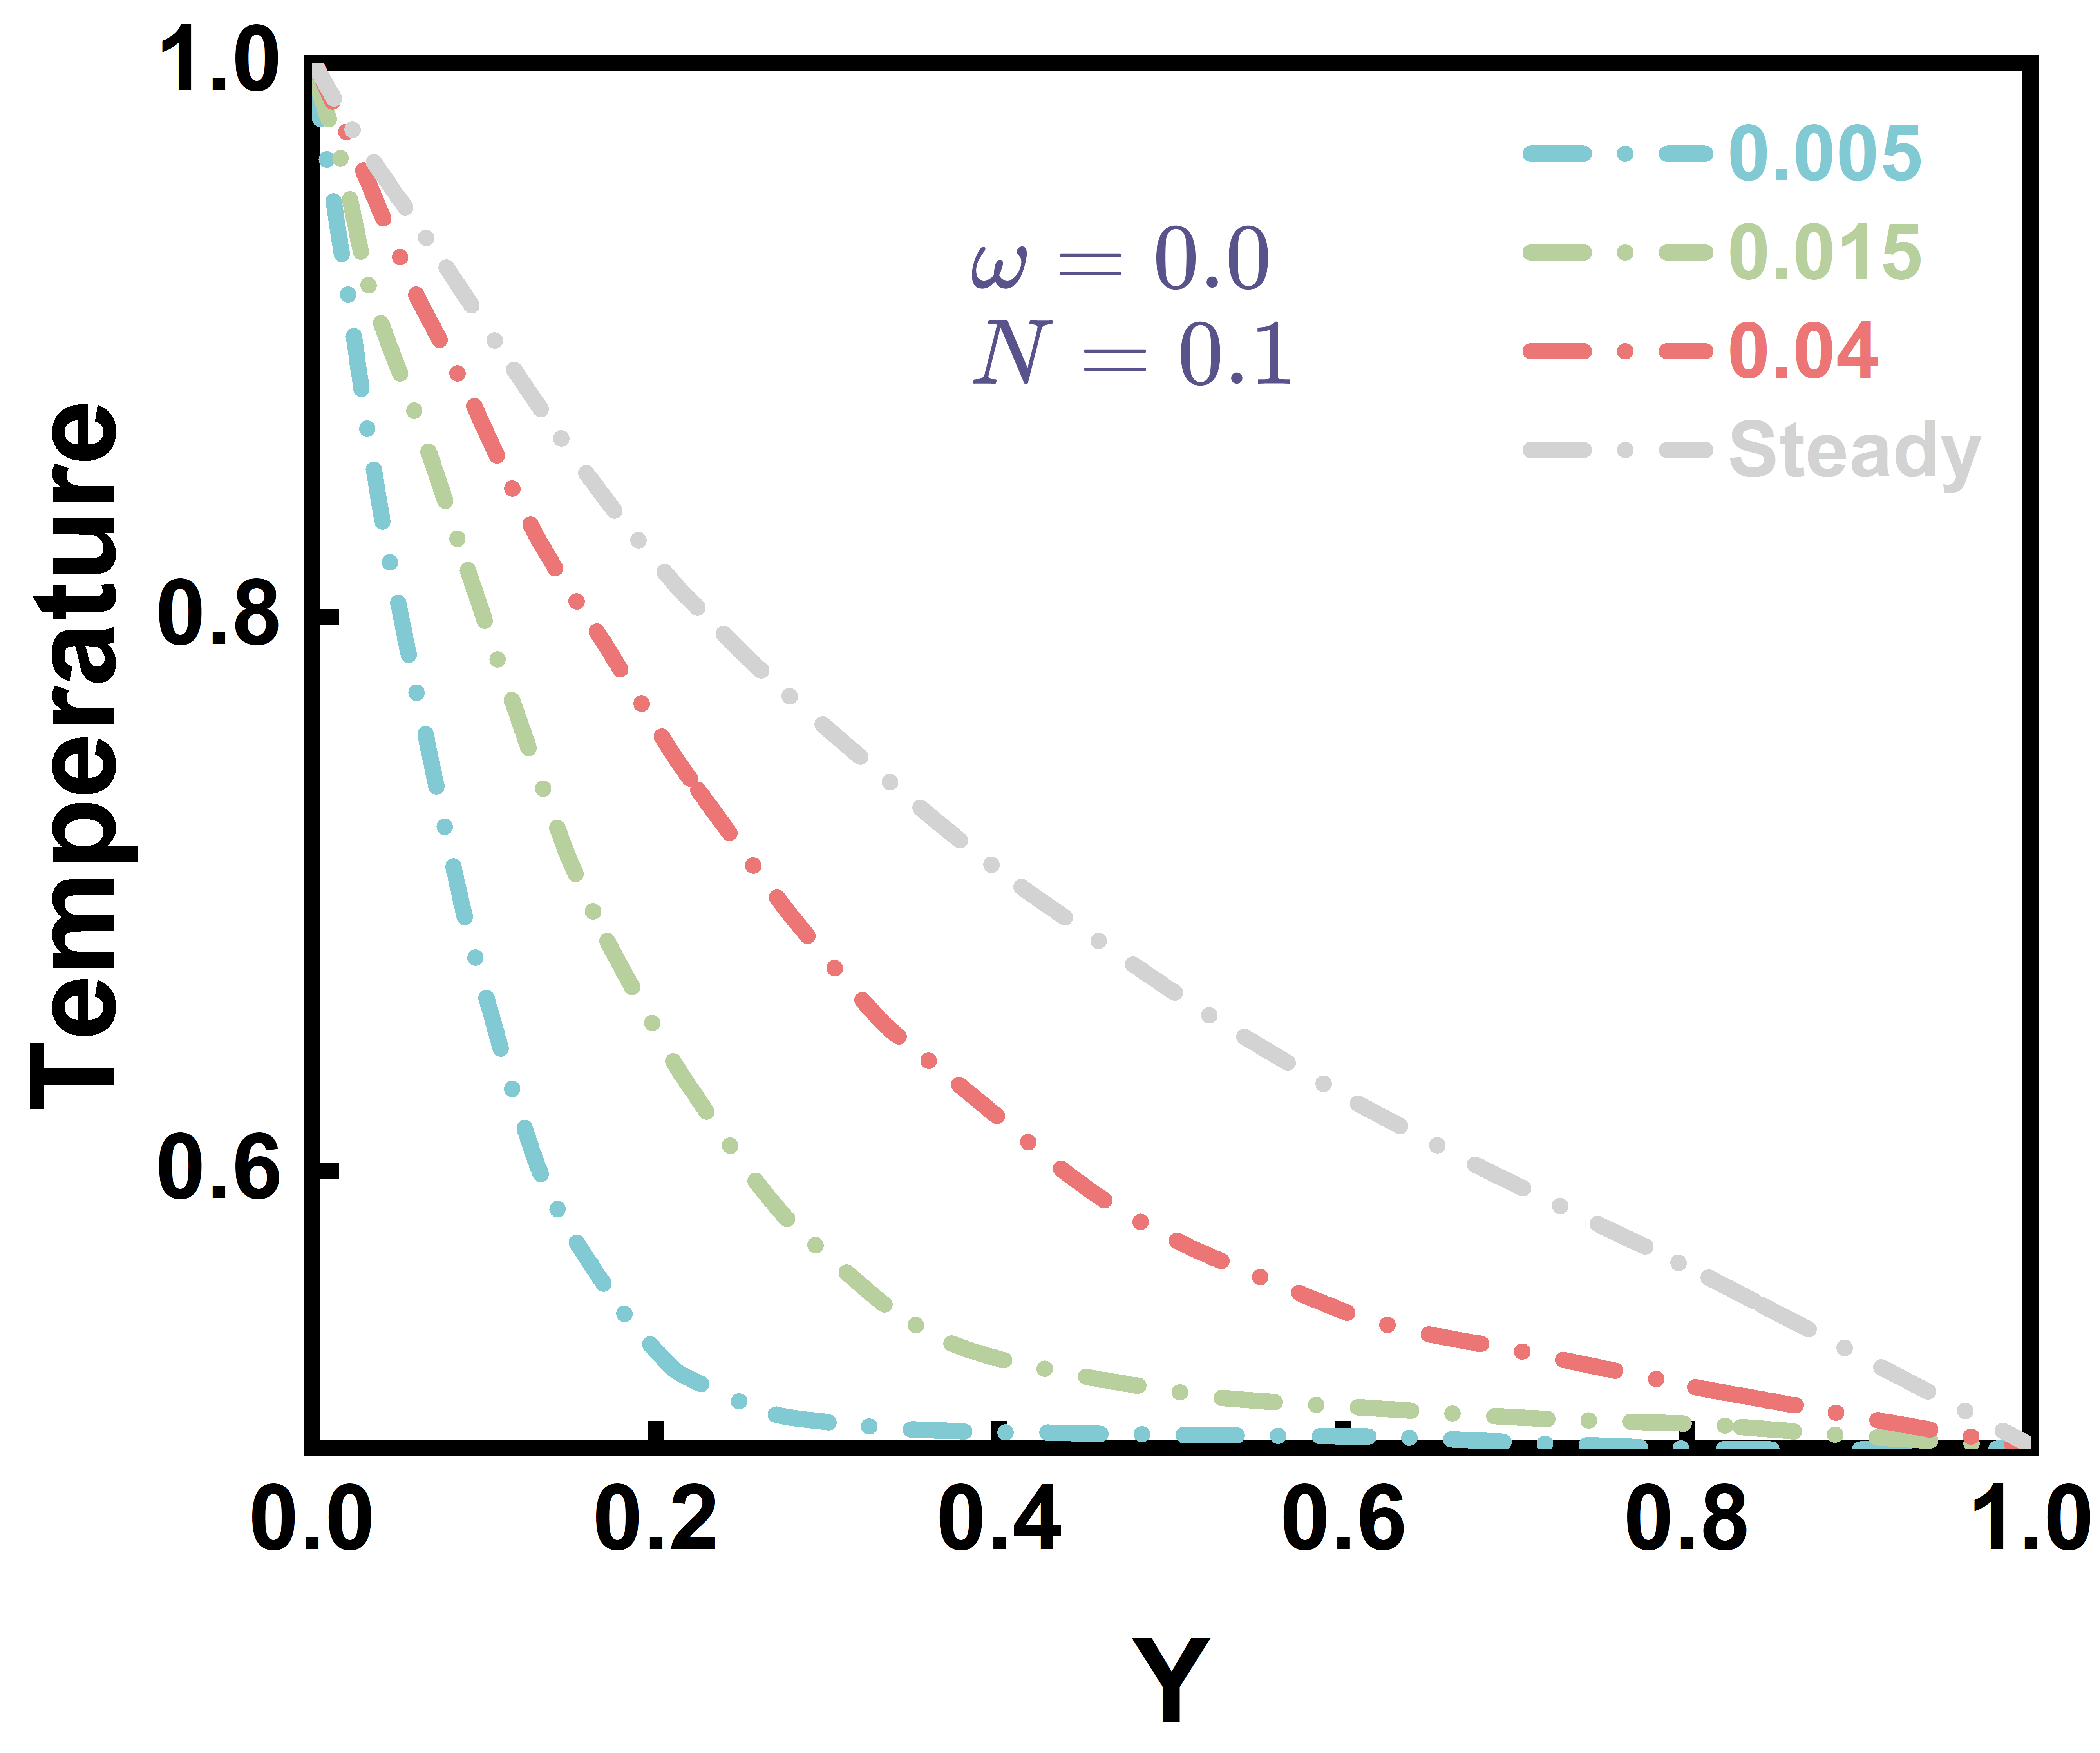
\includegraphics[width=\textwidth]{7B.png}
\caption{}
\end{subfigure}
\hfill
\begin{subfigure}[b]{\figwidth}
\centering
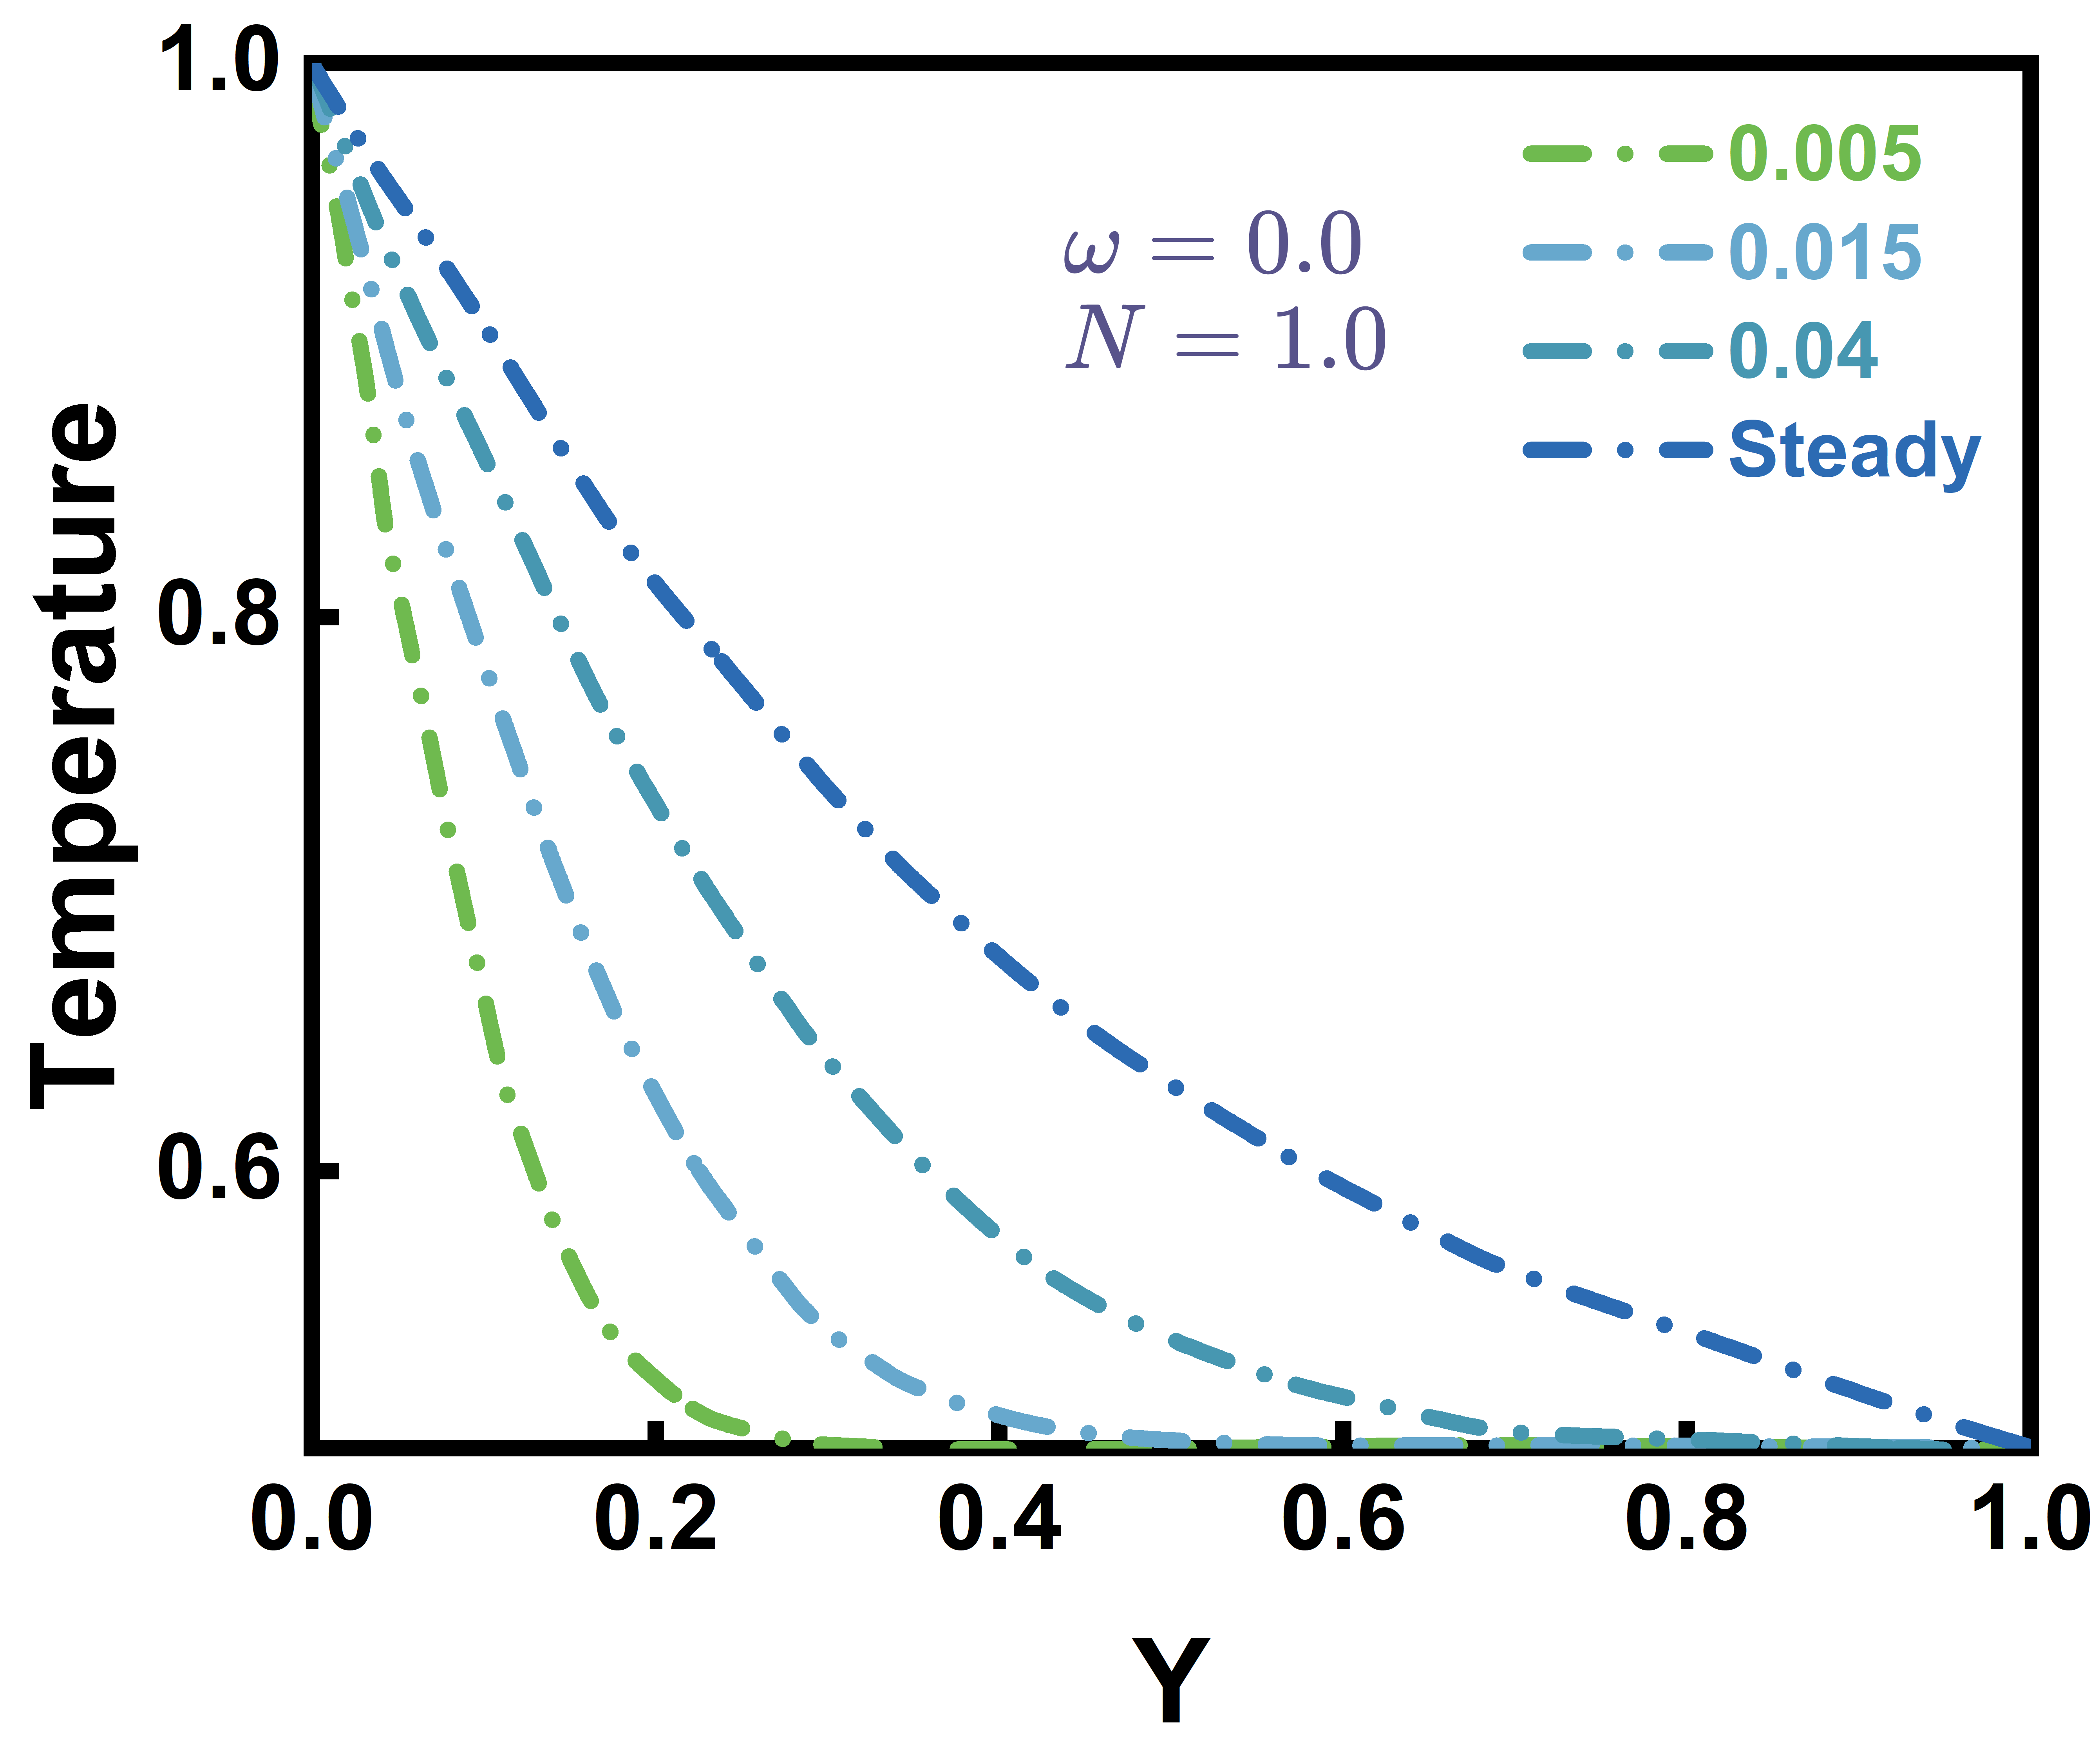
\includegraphics[width=\textwidth]{7C.png}
\caption{}
\end{subfigure}
\caption{Transient centreline temperature profiles in the two-dimensional square enclosure at $\omega=0$. The conduction--radiation parameter is (a) $N=0.01$, (b) $N=0.10$, (c) $N=1.00$.}
\label{fig7}
\end{figure}

Figure~\ref{fig7} shows centreline temperatures at $\omega=0$ for different values of $N$. At $N=0.01$, most of the medium heated rapidly, including at early dimensionless times. At $N=1.00$, early temperature changes remained concentrated near the south wall. Increasing $N$ lowered the centreline temperature and reduced thermal penetration into the upper enclosure. At steady state, the north-wall temperature gradient was larger for smaller $N$.

\subsection{3D cubical-enclosure benchmark}
\label{subsec:3d_cases}

The cubical benchmark tests whether the same coupled DUGKS update remains usable when radiation is transported in all three spatial directions. The physical configuration follows Sun et al.~\cite{SunMaLi2012}: a cubical participating medium occupies $0\leq X,Y,Z\leq1$, all properties are constant, and all six walls are opaque and diffuse-gray. The medium and walls are initially at $H=1$. After heating starts, the south wall is fixed at $H_S=2$, whereas the north, west, east, bottom, and top walls remain at $H=1$. The CSM and LBM--FVM data reported by Sun et al. are used as reference solutions for comparison with the present DUGKS calculations. The governing equations, optical-thickness scaling, and diffuse-gray wall treatment used for this case have been given in Sec.~\ref{subsec:three_dimensional_extension}.

The reported quantities are selected to match the published cubical-enclosure benchmark. Transient isotherms are taken on the centre plane $X=0.5$, and one-dimensional temperature profiles are taken along the centreline $X=0.5$, $Z=0.5$. The retained times are $t^*=0.005$, $0.015$, $0.050$, and steady state. The numerical update uses $H$, while all plotted and tabulated cubical temperatures in this section use the hot-wall-normalised value $\theta=H/2$.

\begin{table}[H]
\centering
\scriptsize
\caption{Three-dimensional cubical-enclosure calculation matrix based on Sun et al.~\cite{SunMaLi2012}. The default setting is $\tau_L=1.0$, $\omega=0$, $N_{cr}=0.01$, and black diffuse walls unless otherwise specified.}
\label{tab:3d_matrix}
\resizebox{\textwidth}{!}{%
\begin{tabular}{@{}p{0.22\textwidth}p{0.38\textwidth}p{0.32\textwidth}@{}}
\toprule
Case group & Parameters & Output quantity \\
\midrule
Baseline transient field & $\tau_L=1.0$, $\omega=0$, $N_{cr}=0.01$, $\varepsilon=1.0$ & Isotherms on $X=0.5$ at $t^*=0.005$, $0.015$, $0.050$, and steady state \\
Scattering albedo effect & $\omega=0.5$ and $0.9$ with $\tau_L=1.0$, $N_{cr}=0.01$, $\varepsilon=1.0$ & Centreline temperature $\theta(Y)=H(Y)/2$ at selected times \\
Conduction--radiation parameter effect & $N_{cr}=0.1$ and $1.0$ with $\tau_L=1.0$, $\omega=0$, $\varepsilon=1.0$ & Centreline temperature $\theta(Y)=H(Y)/2$ at selected times \\
South-wall emissivity effect & $\varepsilon_S=0.1$ and $0.5$ with $\tau_L=1.0$, $\omega=0$, $N_{cr}=0.01$ & Centreline temperature $\theta(Y)=H(Y)/2$ at selected times \\
Optical-thickness effect & $\tau_L=0.1$ and $5.0$ with $\omega=0$, $N_{cr}=0.01$, $\varepsilon=1.0$ & Centreline temperature $\theta(Y)=H(Y)/2$ at selected times \\
\bottomrule
\end{tabular}%
}
\end{table}

The calculations listed in Table~\ref{tab:3d_matrix} use the D3Q27 thermal velocity set and a three-component angular finite-volume quadrature with $N_\theta=8$ and $N_\phi=16$. The cell-centred mesh contains $31^3$ control volumes. Steady state is defined by a maximum temperature change below $5\times10^{-7}$ between successive physical time steps. Sun et al.~\cite{SunMaLi2012} used their Table 1 to examine node and angular-direction sensitivity for the same baseline condition. The present calculation does not repeat that full refinement matrix. Instead, Table~\ref{tab:sun2012_table1_present} reports a representative pointwise comparison at the three centreline locations listed in their table, using the Sun et al. CSM data as the literature reference and the present DUGKS result as the corresponding calculation on the retained mesh.

\begin{table}[H]
\centering
\scriptsize
\caption{Representative comparison with the centreline data in Table 1 of Sun et al.~\cite{SunMaLi2012} at $t^*=0.005$, $N_{cr}=0.01$, $\tau_L=1.0$, $\omega=0$, and $\varepsilon=1.0$. Values are hot-wall-normalised temperatures on $X=0.5$, $Z=0.5$. The CSM values are taken from the $14\times14\times14$, $S_8$ row used by Sun et al. for their subsequent calculations. The present data are computed on the $31^3$ finite-volume mesh used for the three-dimensional DUGKS calculations.}
\label{tab:sun2012_table1_present}
\begin{tabular}{@{}c c c c c@{}}
\toprule
$Y$ & Sun et al. CSM & Present DUGKS & Absolute difference & Relative difference \\
\midrule
0.25 & 0.59916 & 0.59602 & $3.14\times10^{-3}$ & 0.52\% \\
0.50 & 0.54097 & 0.54186 & $8.86\times10^{-4}$ & 0.16\% \\
0.75 & 0.51635 & 0.52042 & $4.07\times10^{-3}$ & 0.79\% \\
\bottomrule
\end{tabular}
\end{table}

The pointwise differences in Table~\ref{tab:sun2012_table1_present} remain below $4.1\times10^{-3}$ for the three sampled locations. This comparison is used only as a baseline benchmark check, because spatial and angular convergence for the present three-dimensional calculation has not been independently established.

\begin{figure}[H]
\centering
\begin{subfigure}[b]{0.48\textwidth}
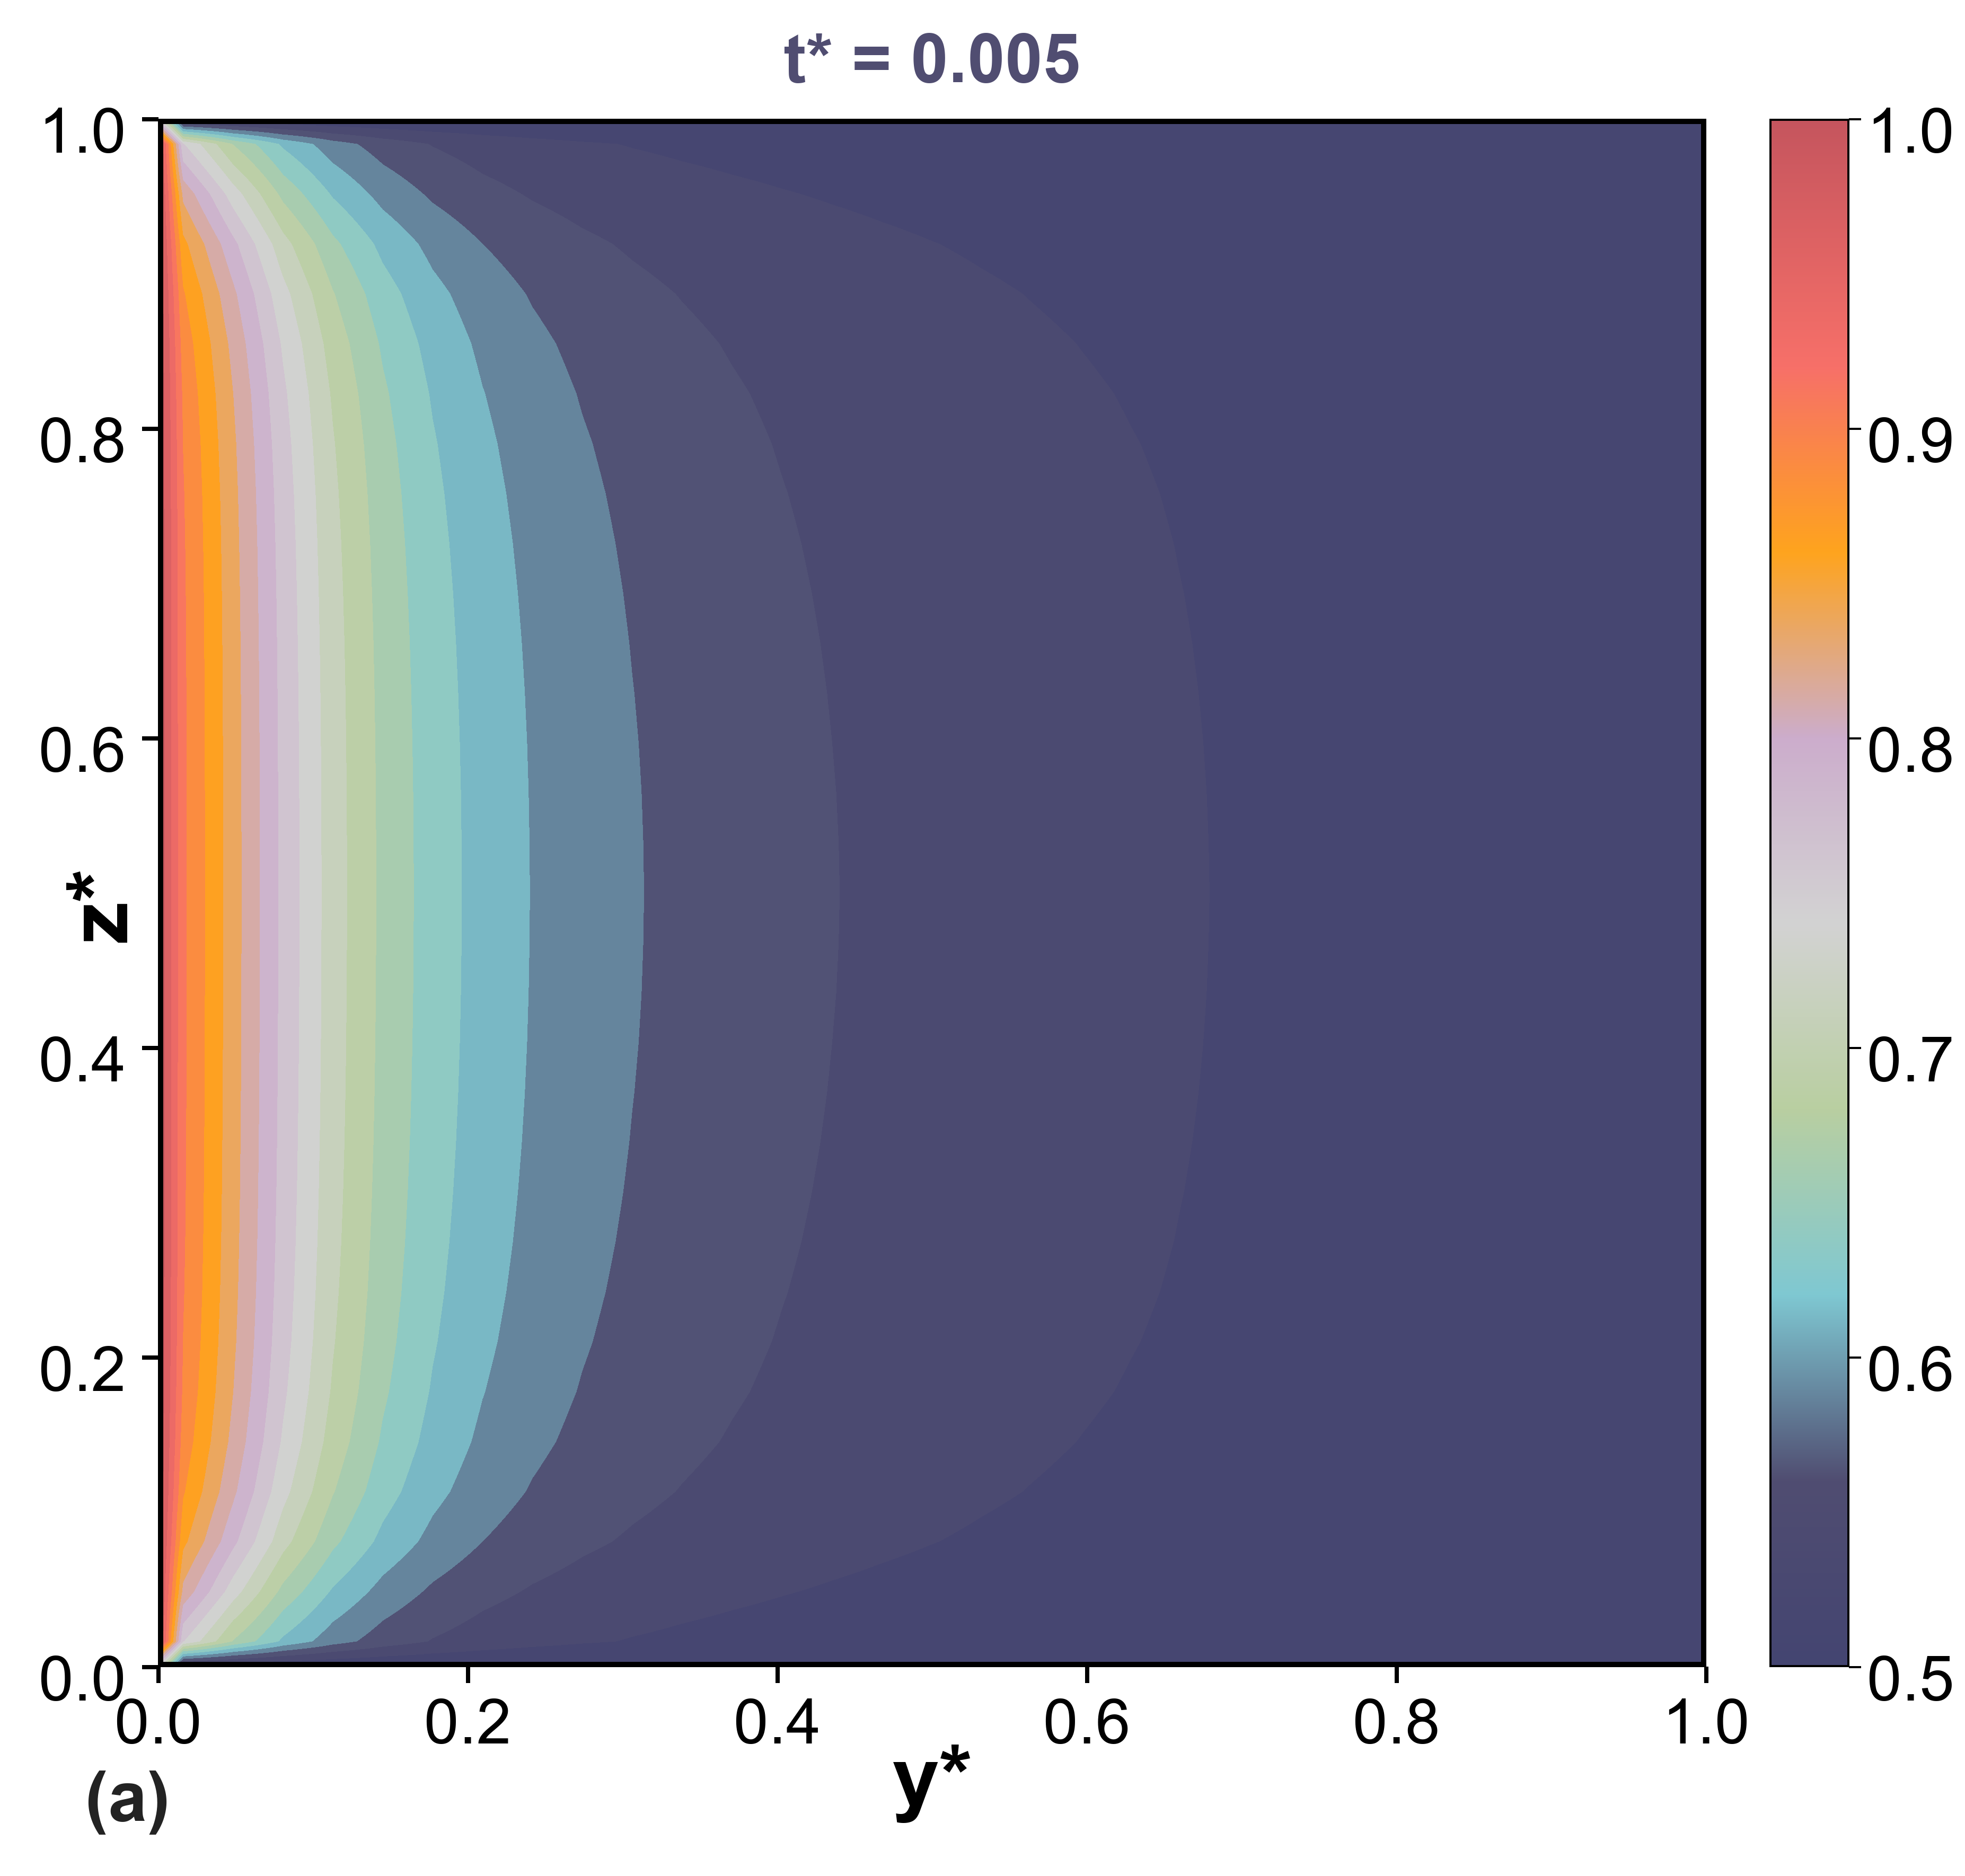
\includegraphics[width=\textwidth]{8A.png}
\caption{}
\end{subfigure}\hfill
\begin{subfigure}[b]{0.48\textwidth}
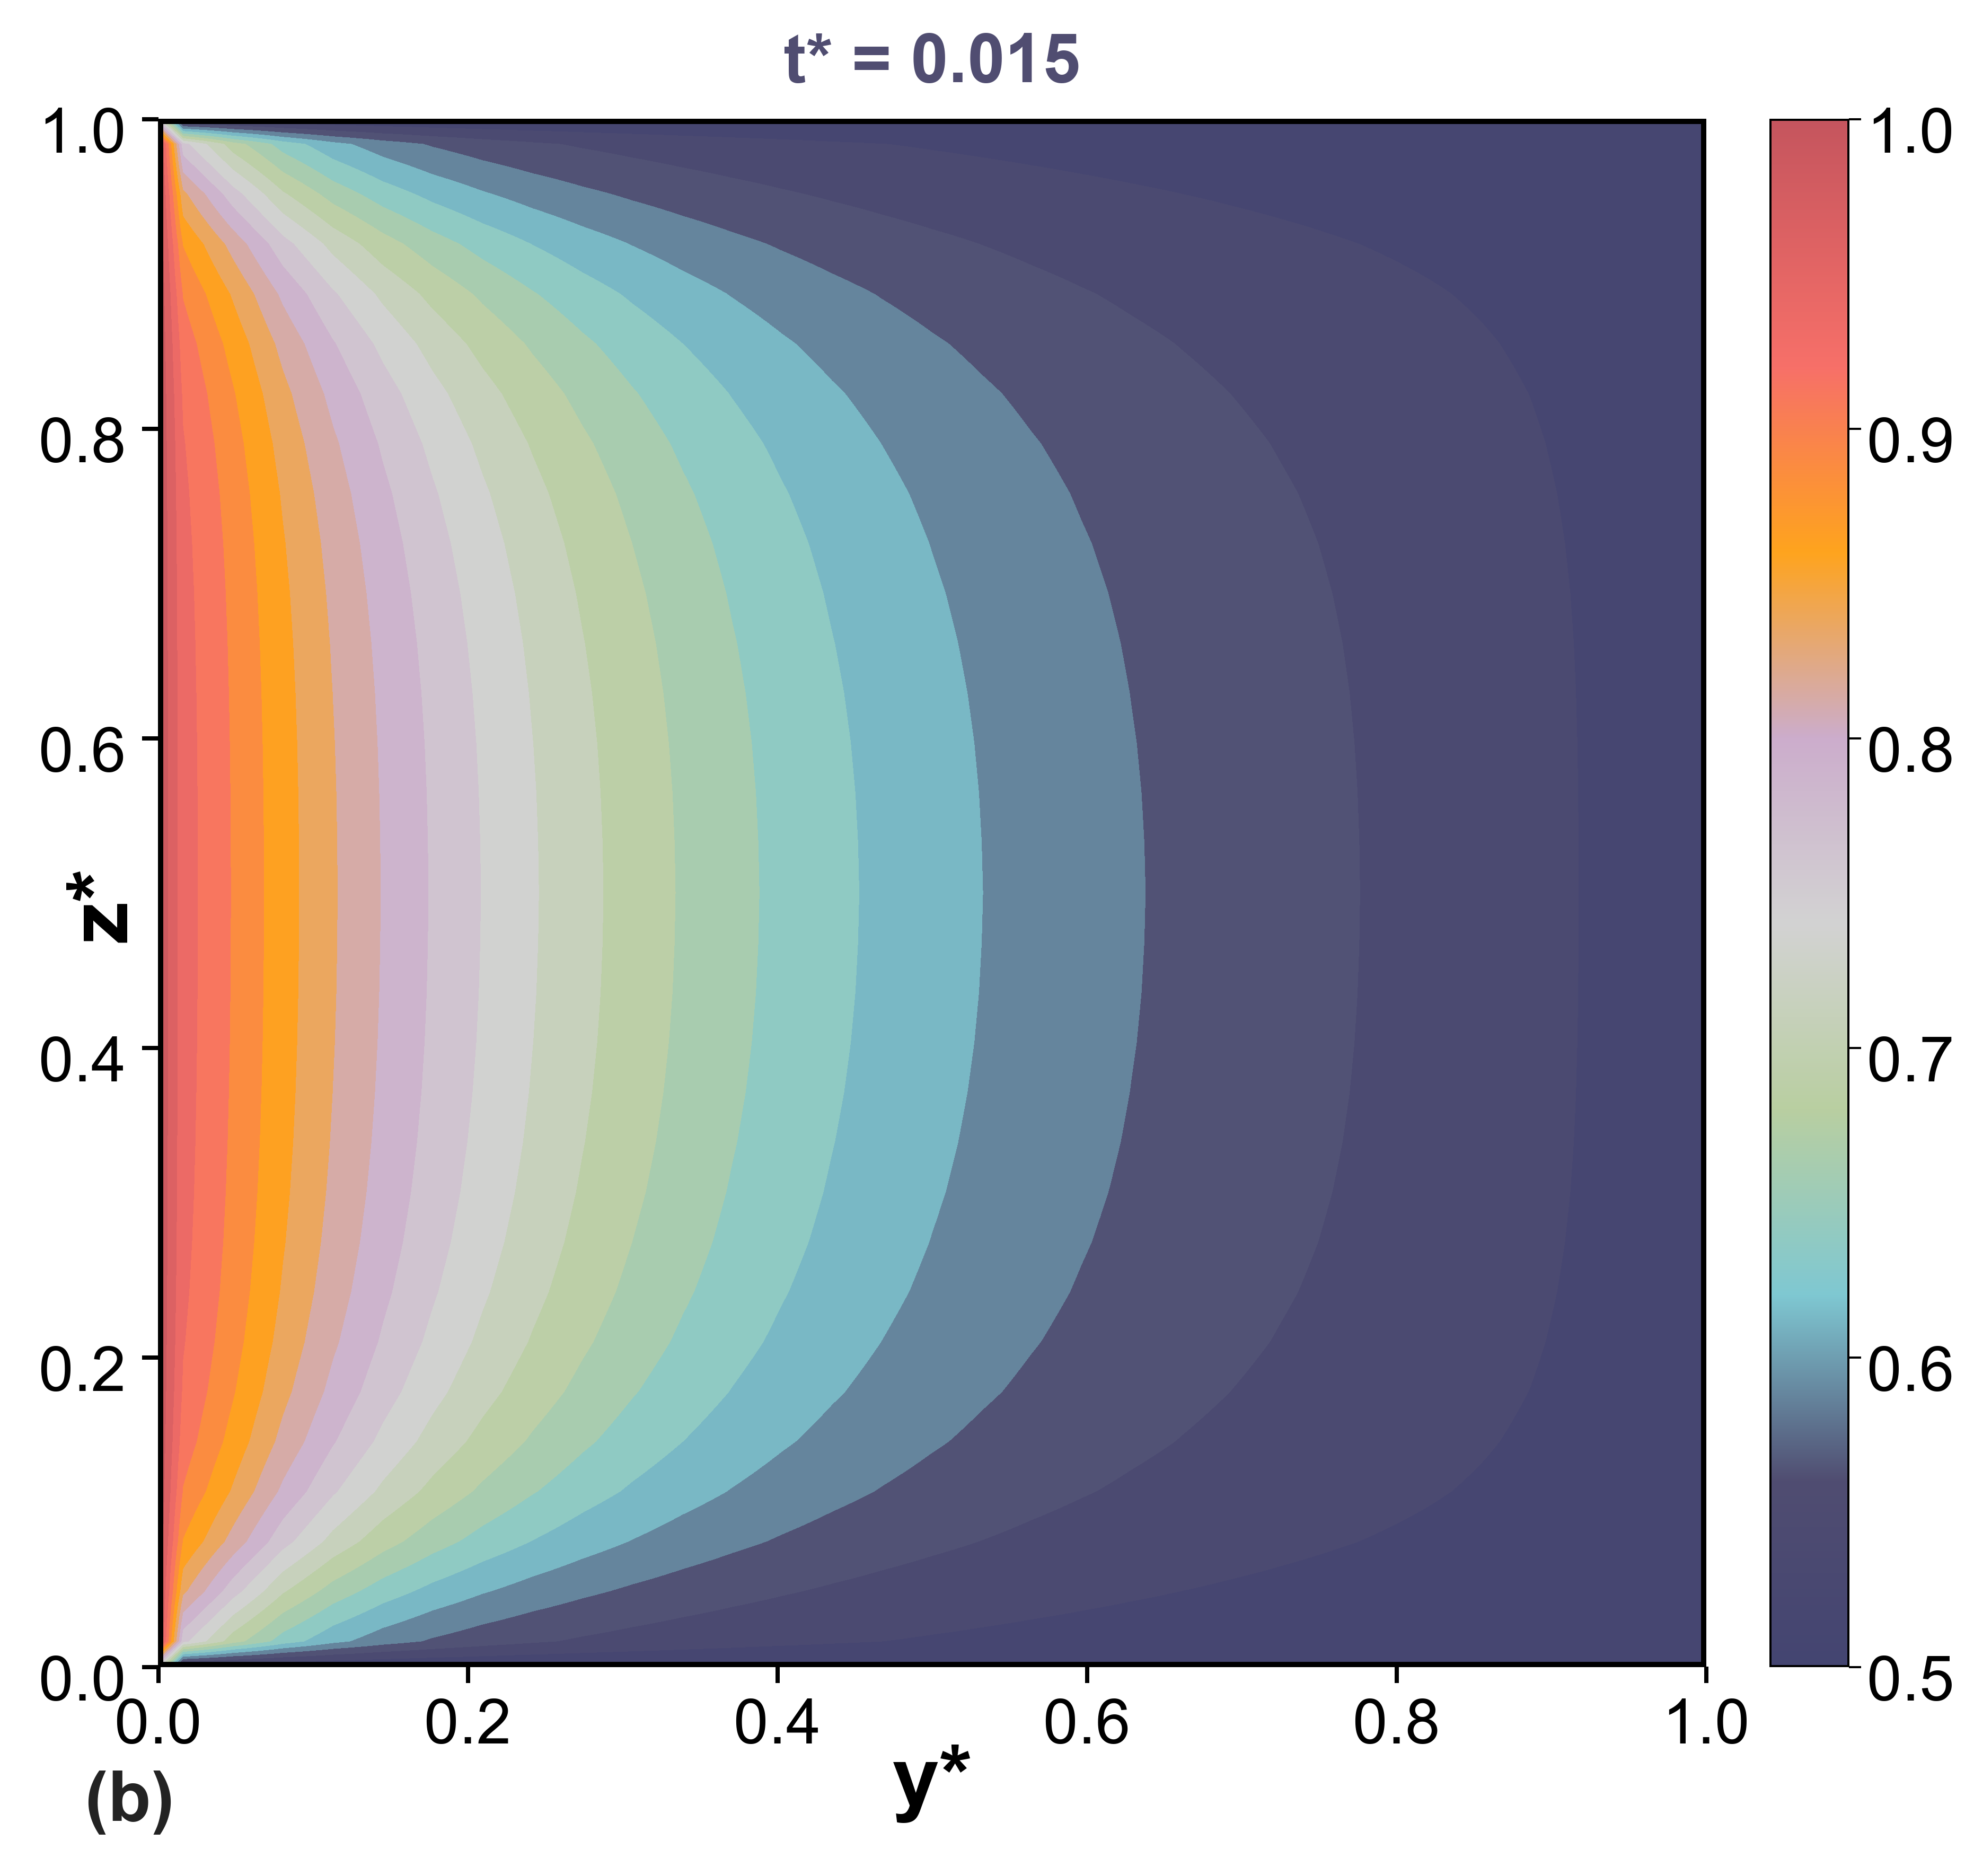
\includegraphics[width=\textwidth]{8B.png}
\caption{}
\end{subfigure}

\begin{subfigure}[b]{0.48\textwidth}
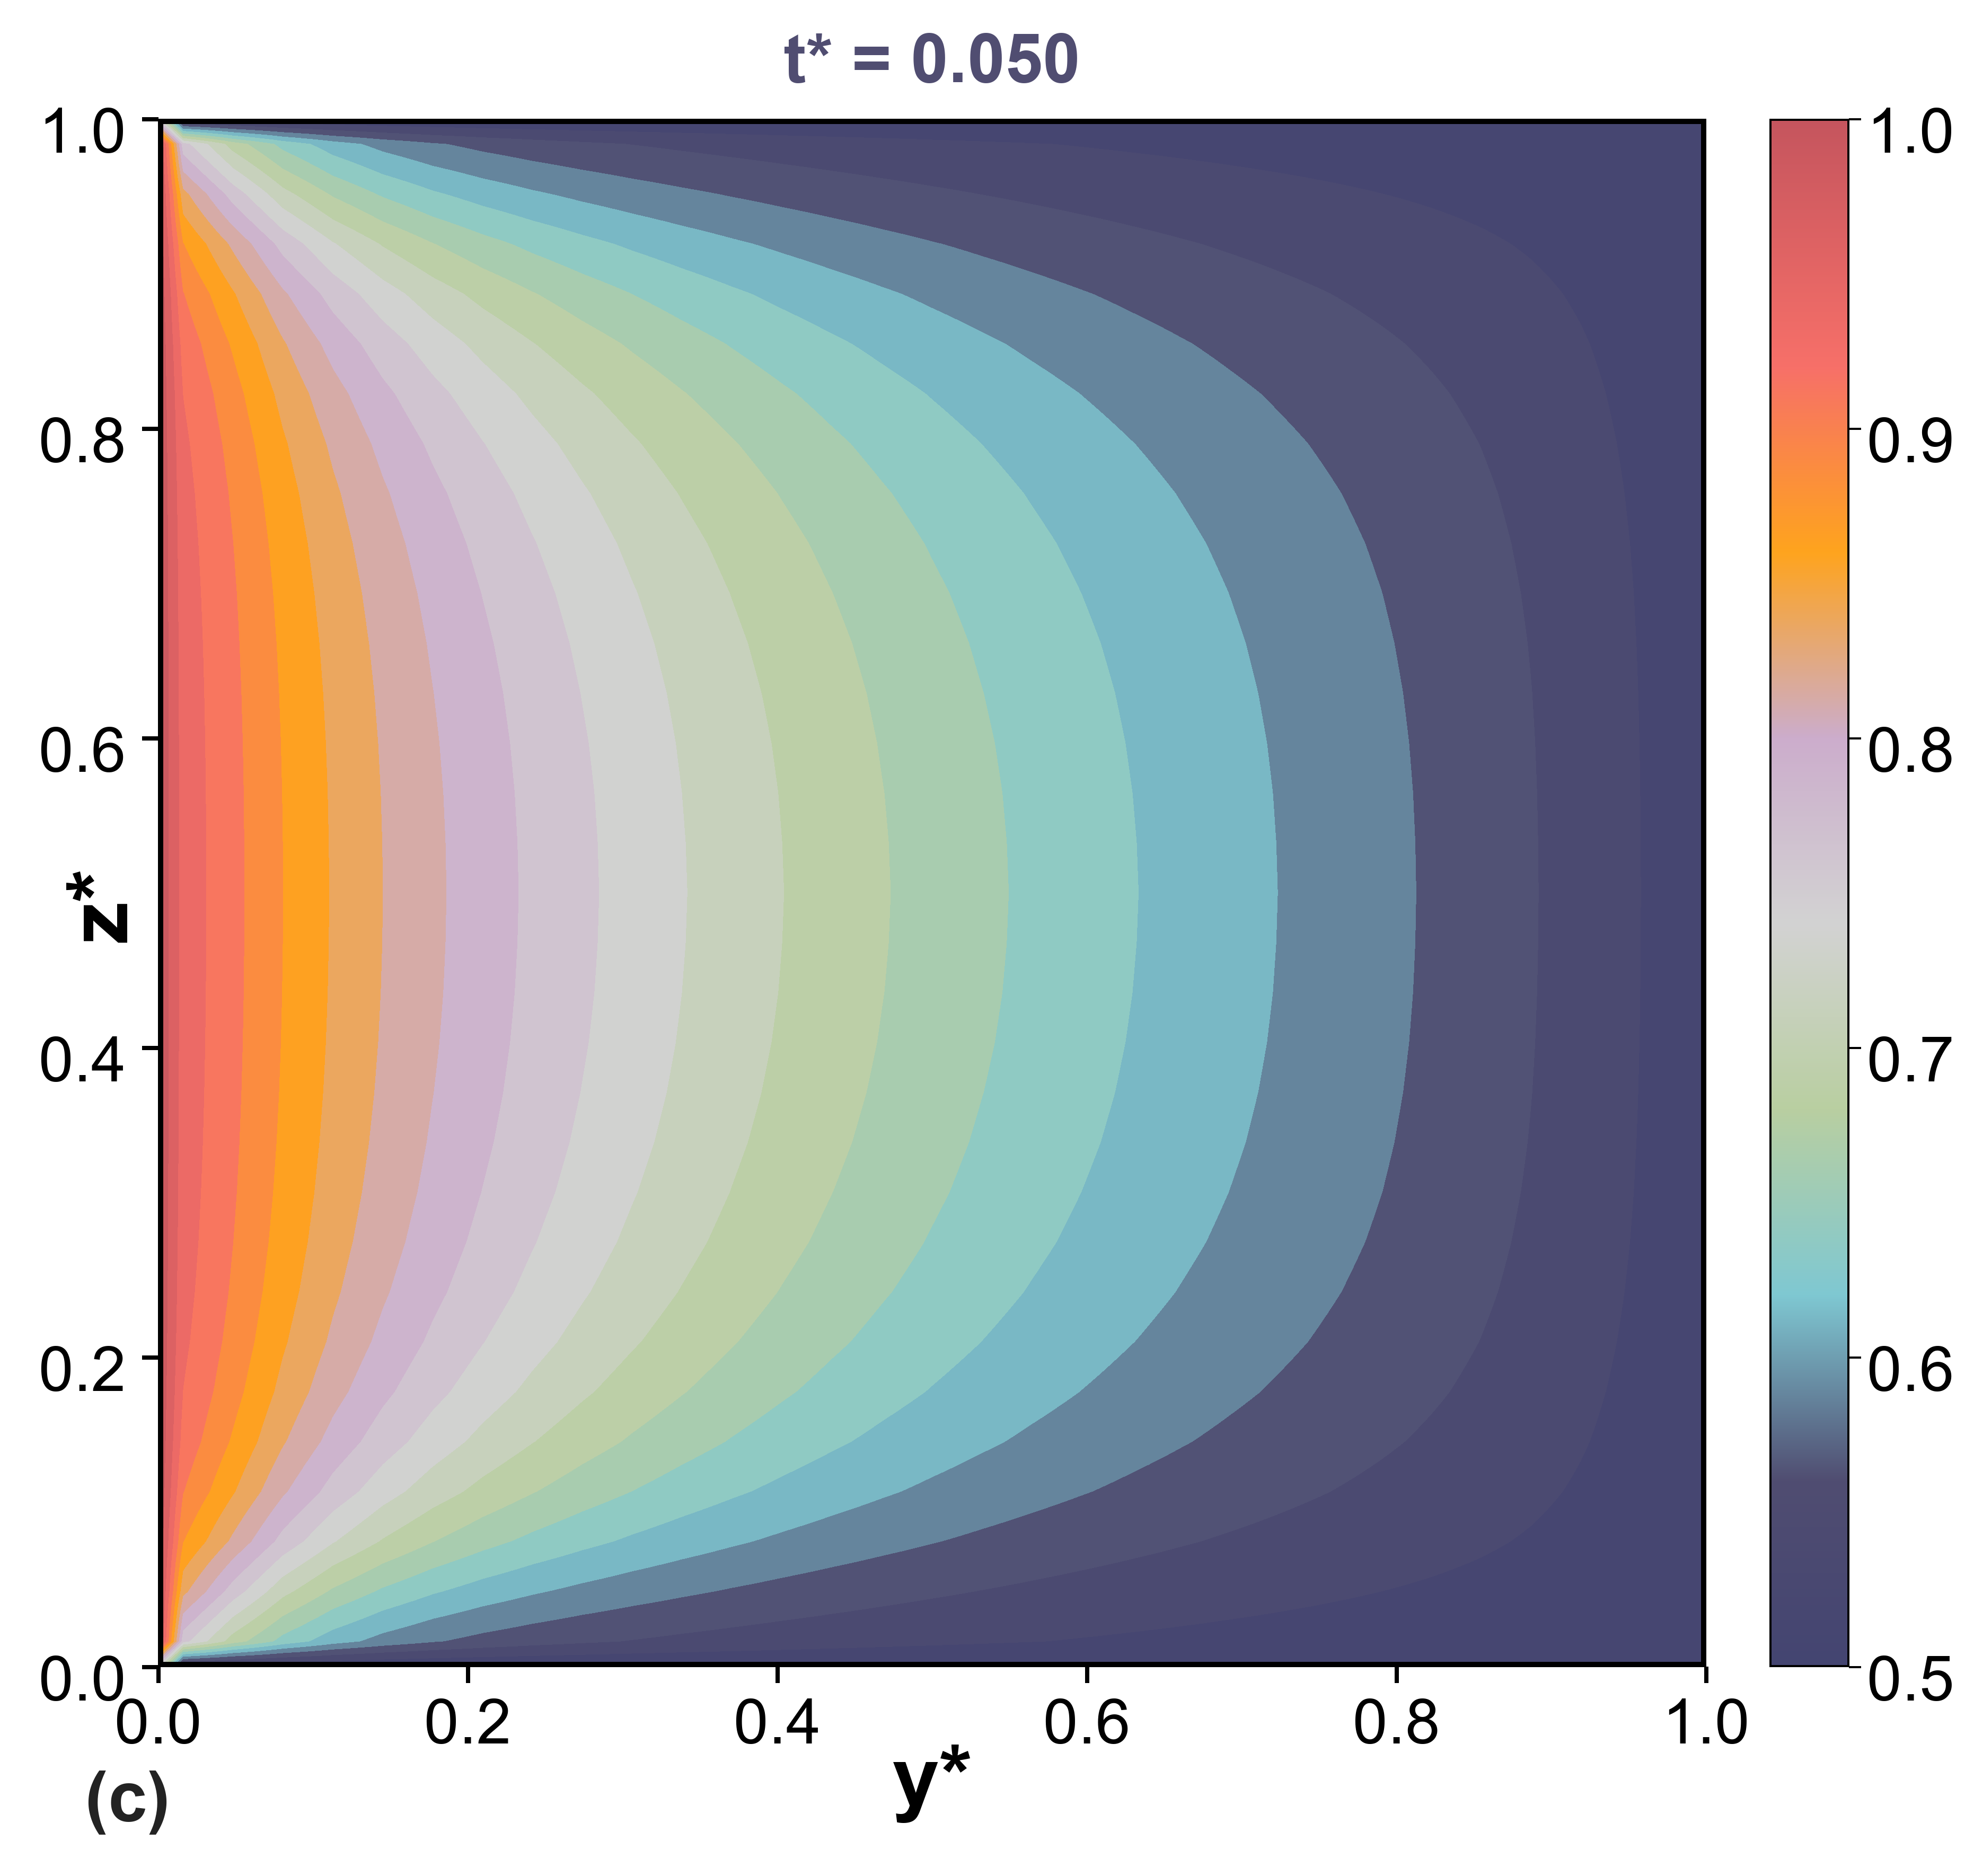
\includegraphics[width=\textwidth]{8C.png}
\caption{}
\end{subfigure}\hfill
\begin{subfigure}[b]{0.48\textwidth}
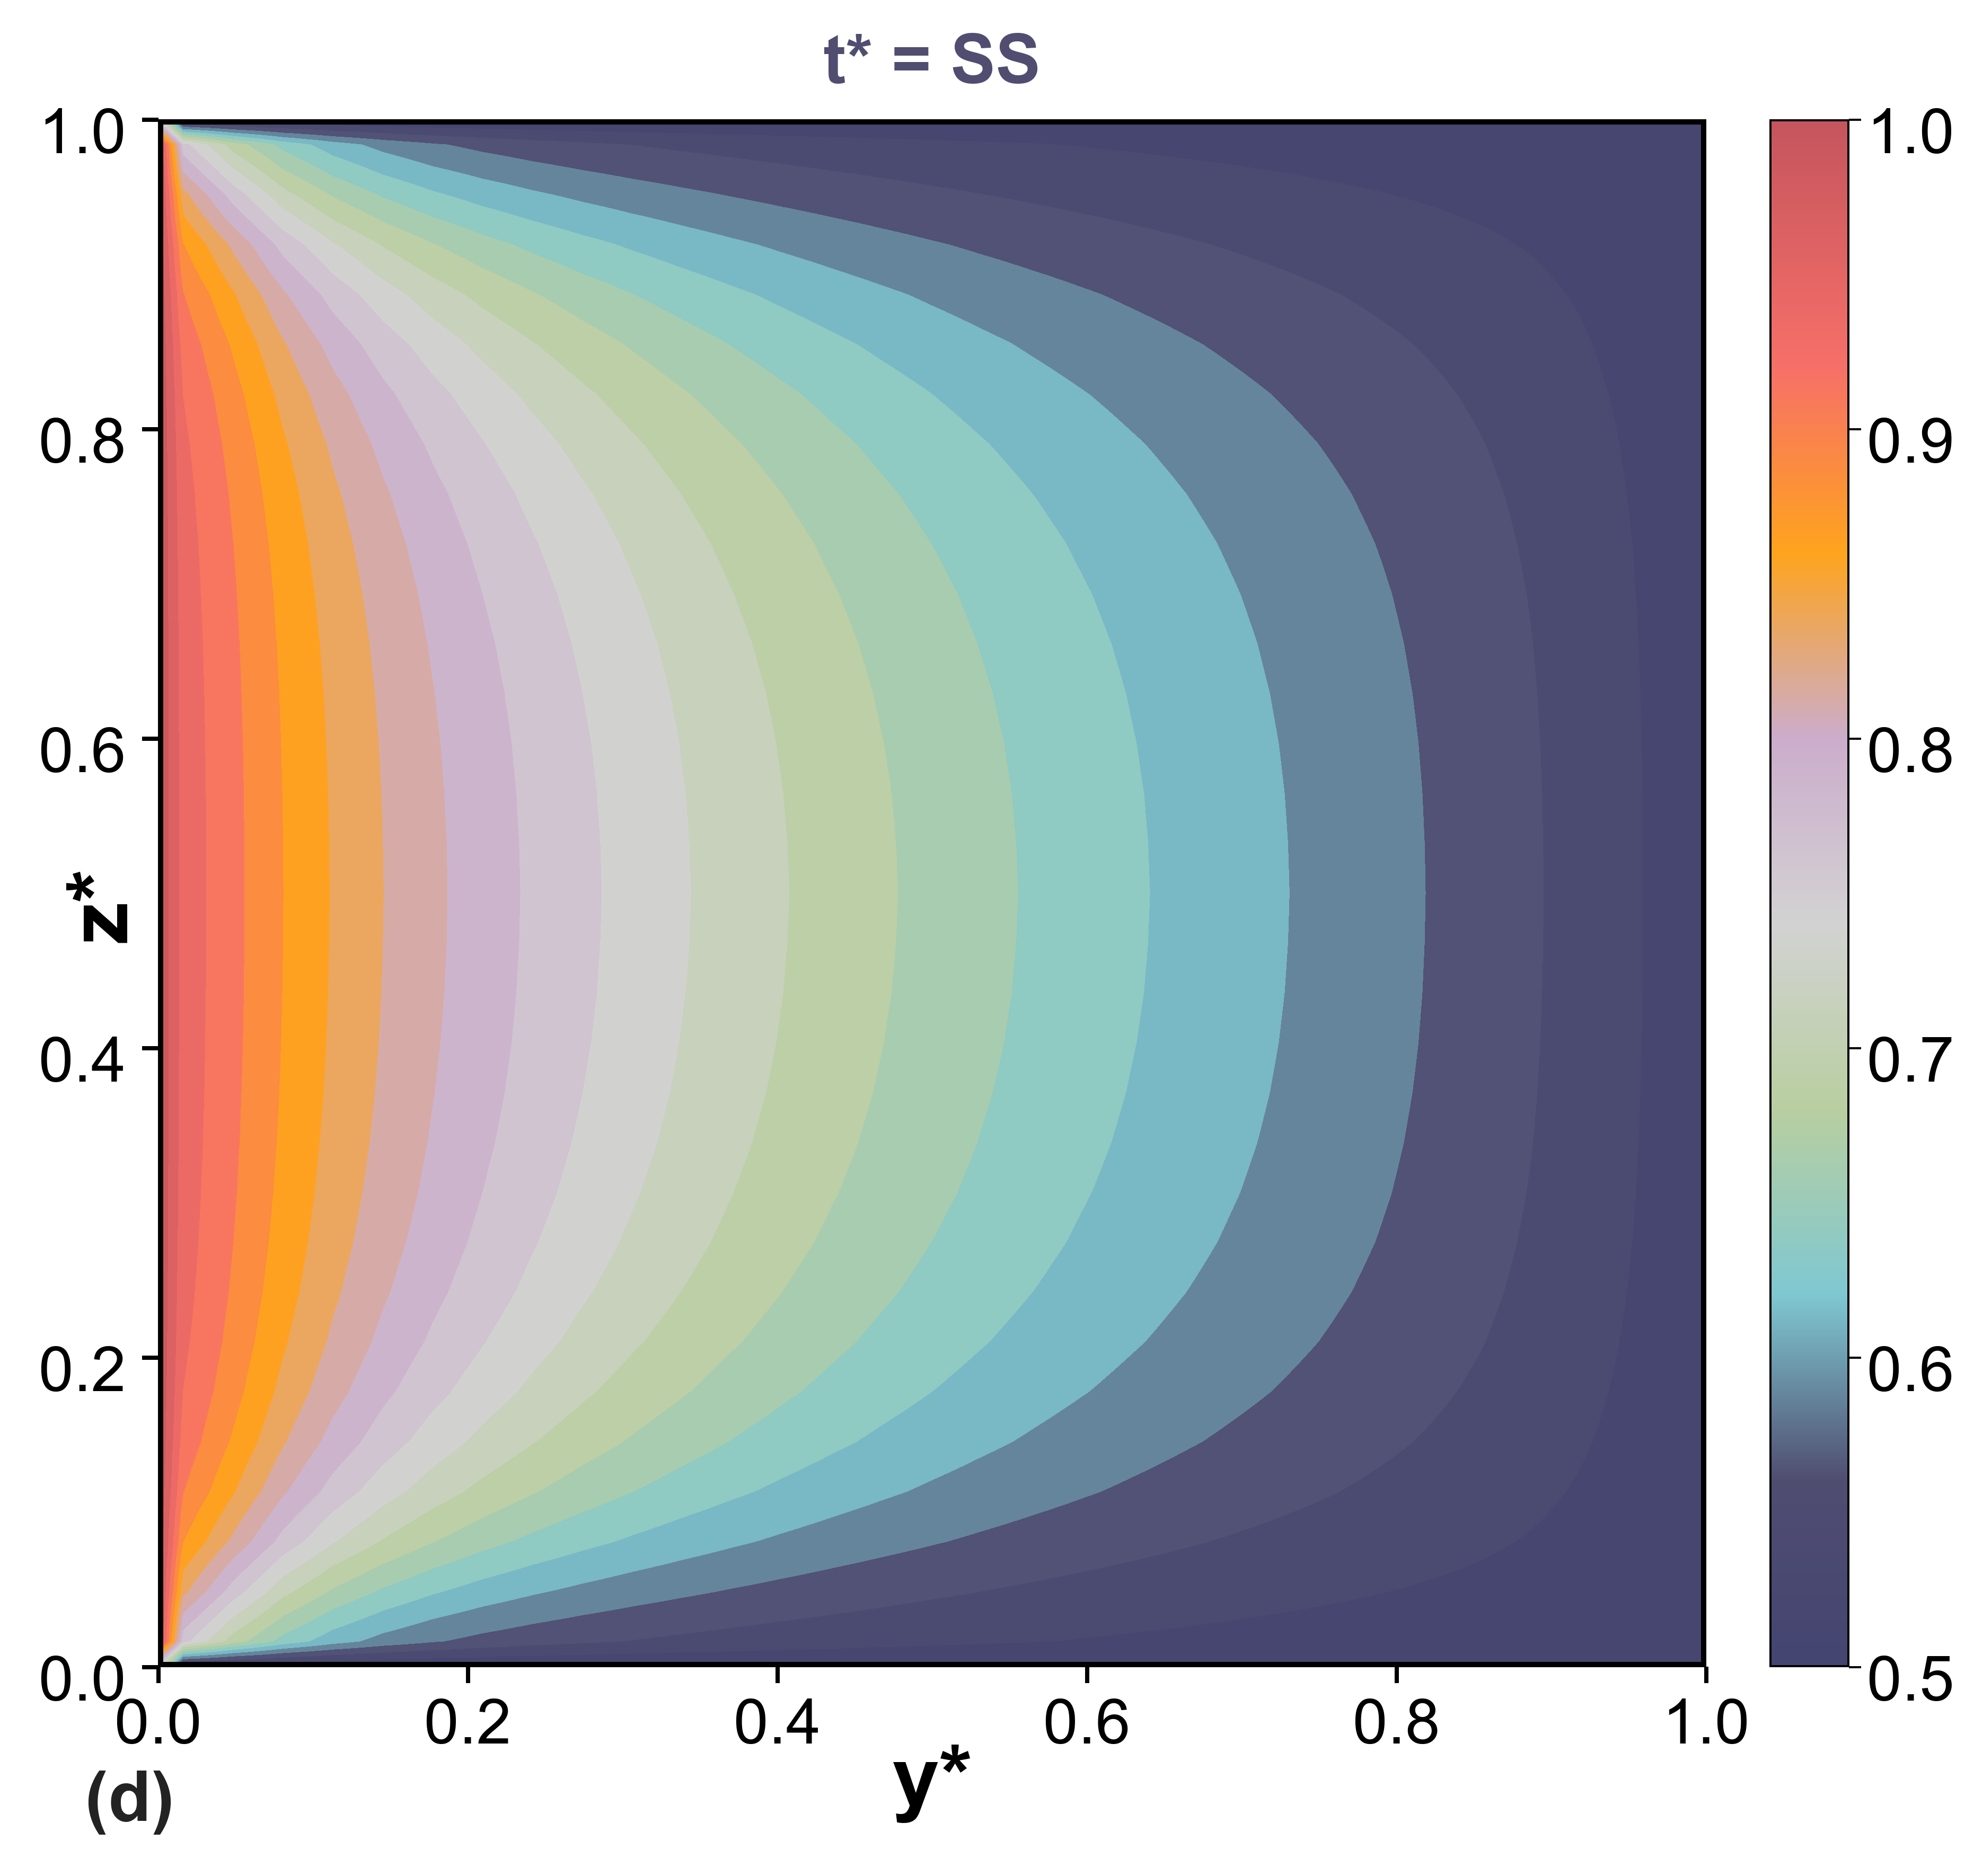
\includegraphics[width=\textwidth]{8D.png}
\caption{}
\end{subfigure}
\caption{Transient isotherms on the centre plane $X=0.5$ for the baseline cubical enclosure. The case uses $\tau_L=1.0$, $\omega=0$, $\varepsilon=1.0$, and $N_{cr}=0.01$. The retained times are shown in the panels.}
\label{fig8}
\end{figure}

Figure~\ref{fig8} follows the baseline isotherm sequence reported by Sun et al.~\cite{SunMaLi2012}. The hot south wall first produces a steep thermal layer near $Y=0$, and the high-temperature region then penetrates towards the enclosure interior. The contours remain symmetric about the mid-plane in $Z$, which is consistent with the identical bottom and top wall temperatures. The centre point $(X,Y,Z)=(0.5,0.5,0.5)$ warmed from $\theta=0.542$ at $t^*=0.005$ to $\theta=0.668$ at steady state.

\begin{figure}[H]
\centering
\begin{subfigure}[b]{0.48\textwidth}
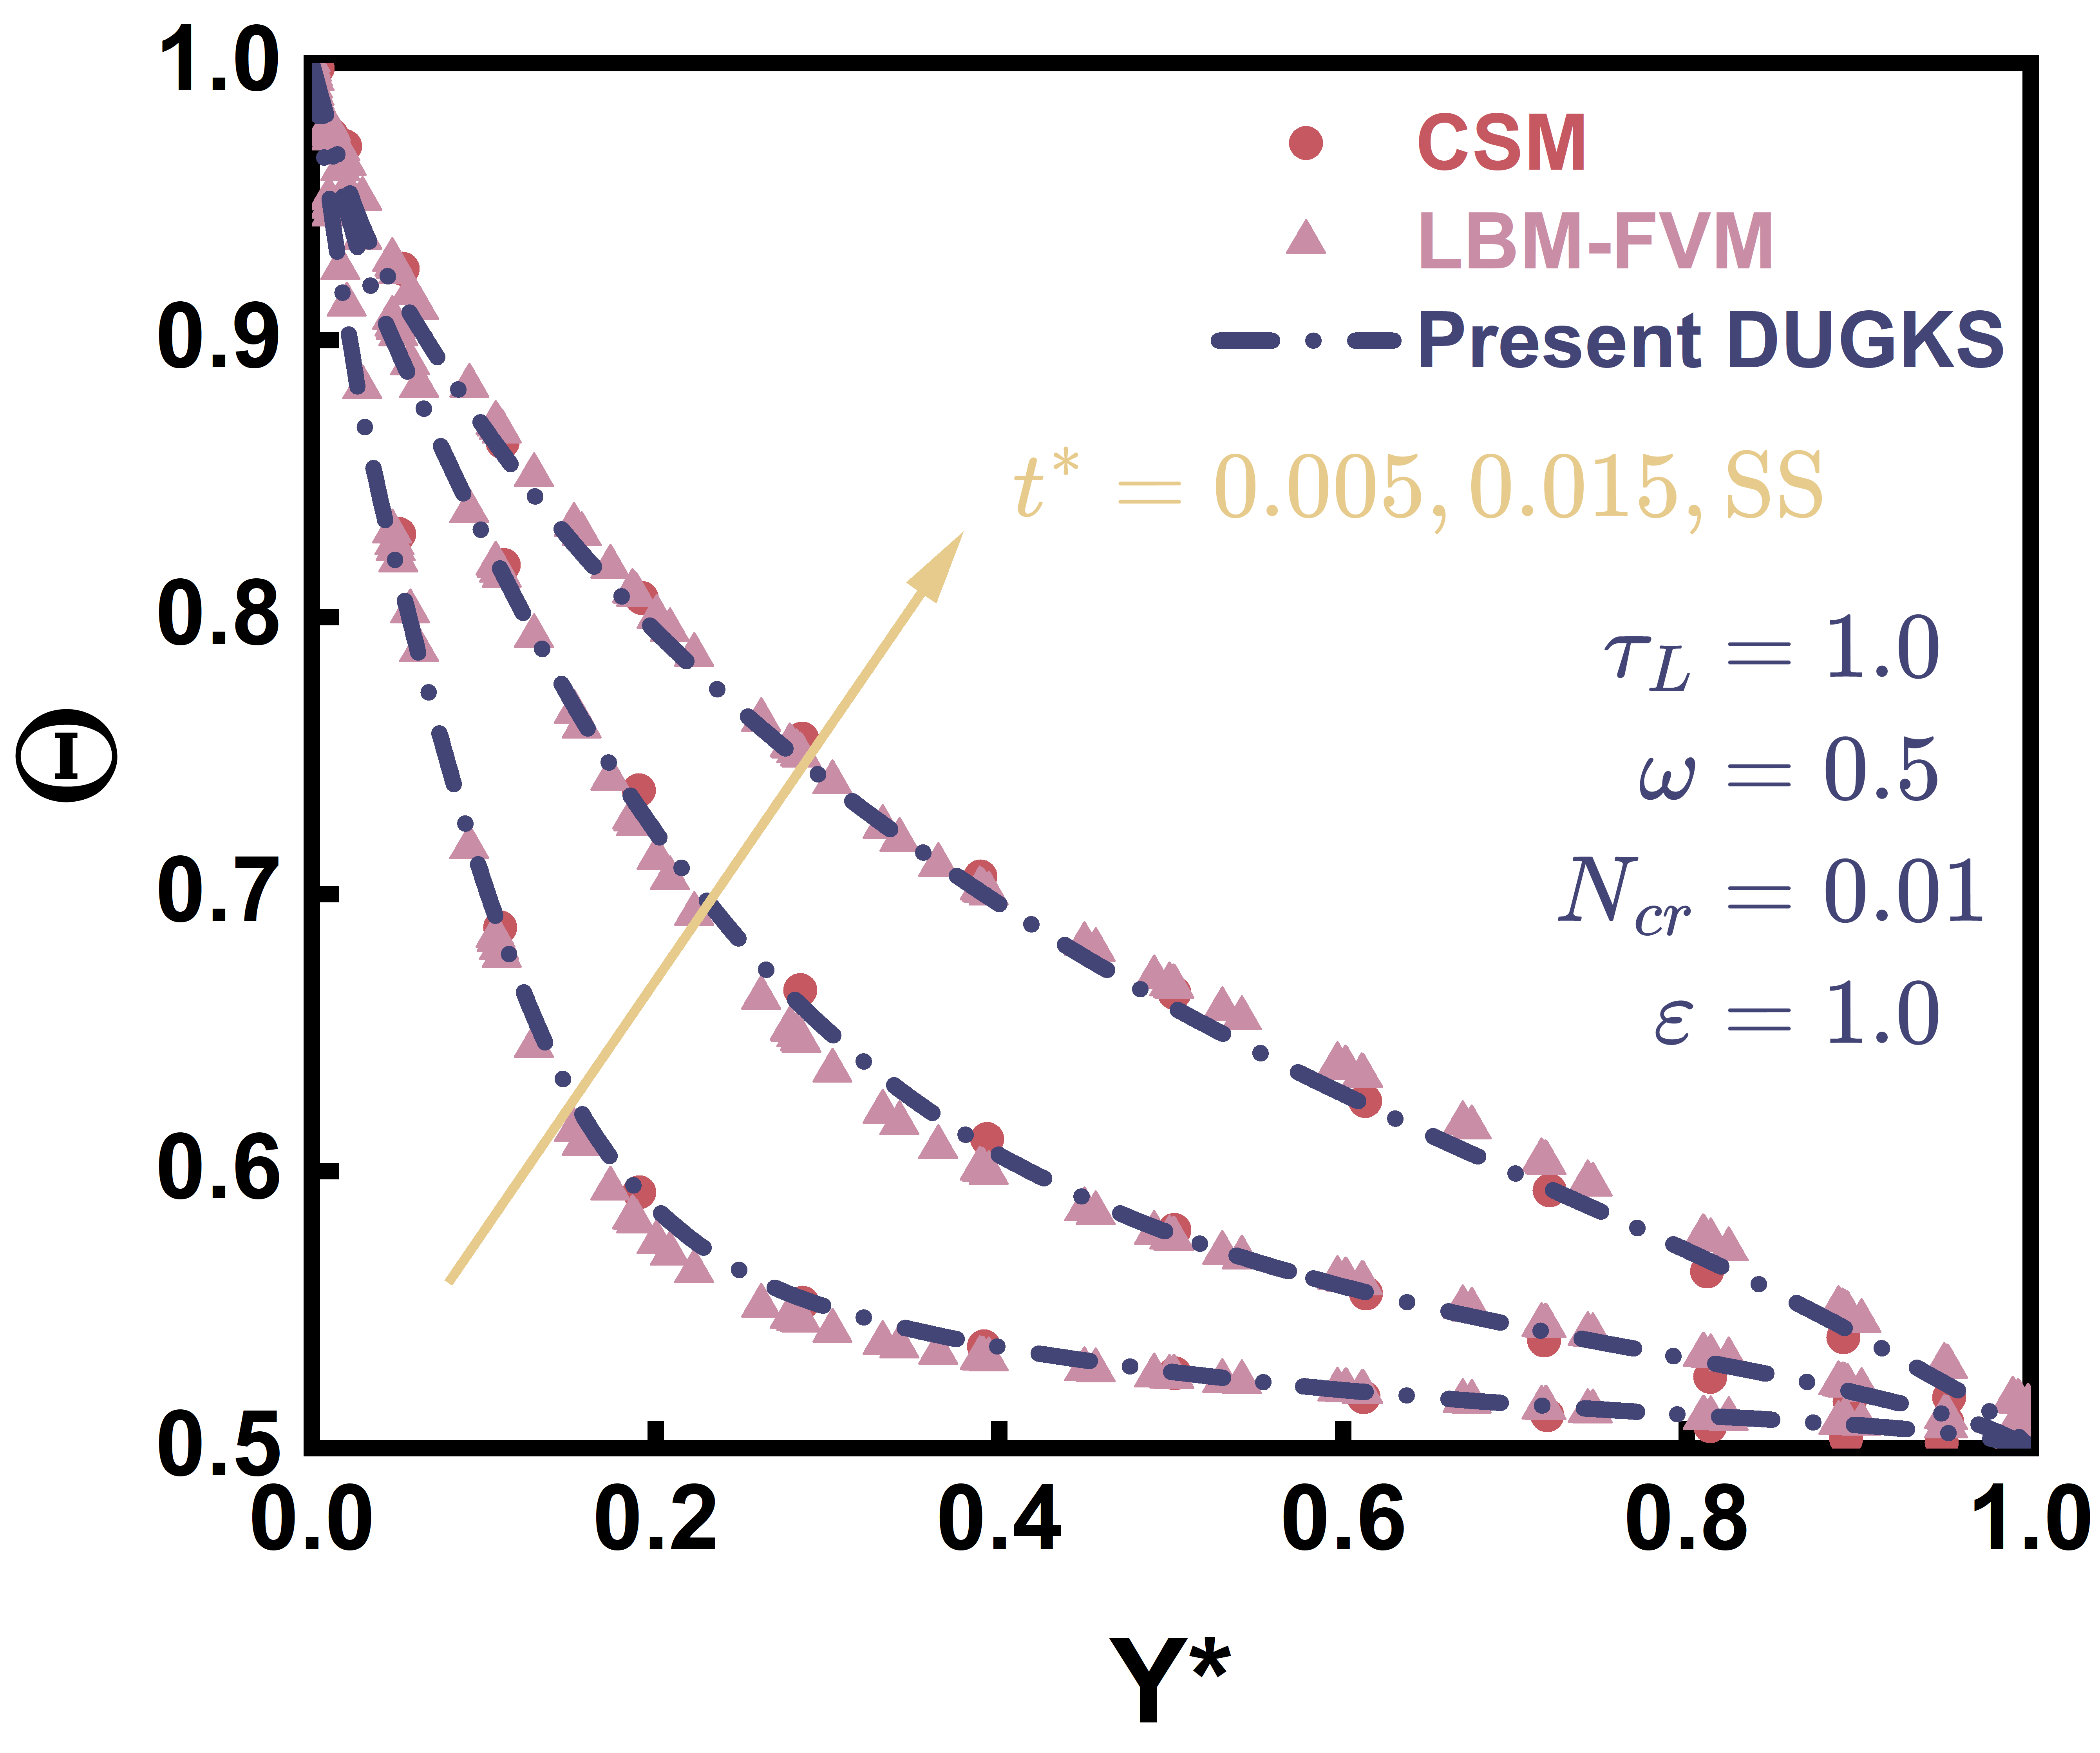
\includegraphics[width=\textwidth]{9A.png}
\caption{}
\end{subfigure}\hfill
\begin{subfigure}[b]{0.48\textwidth}
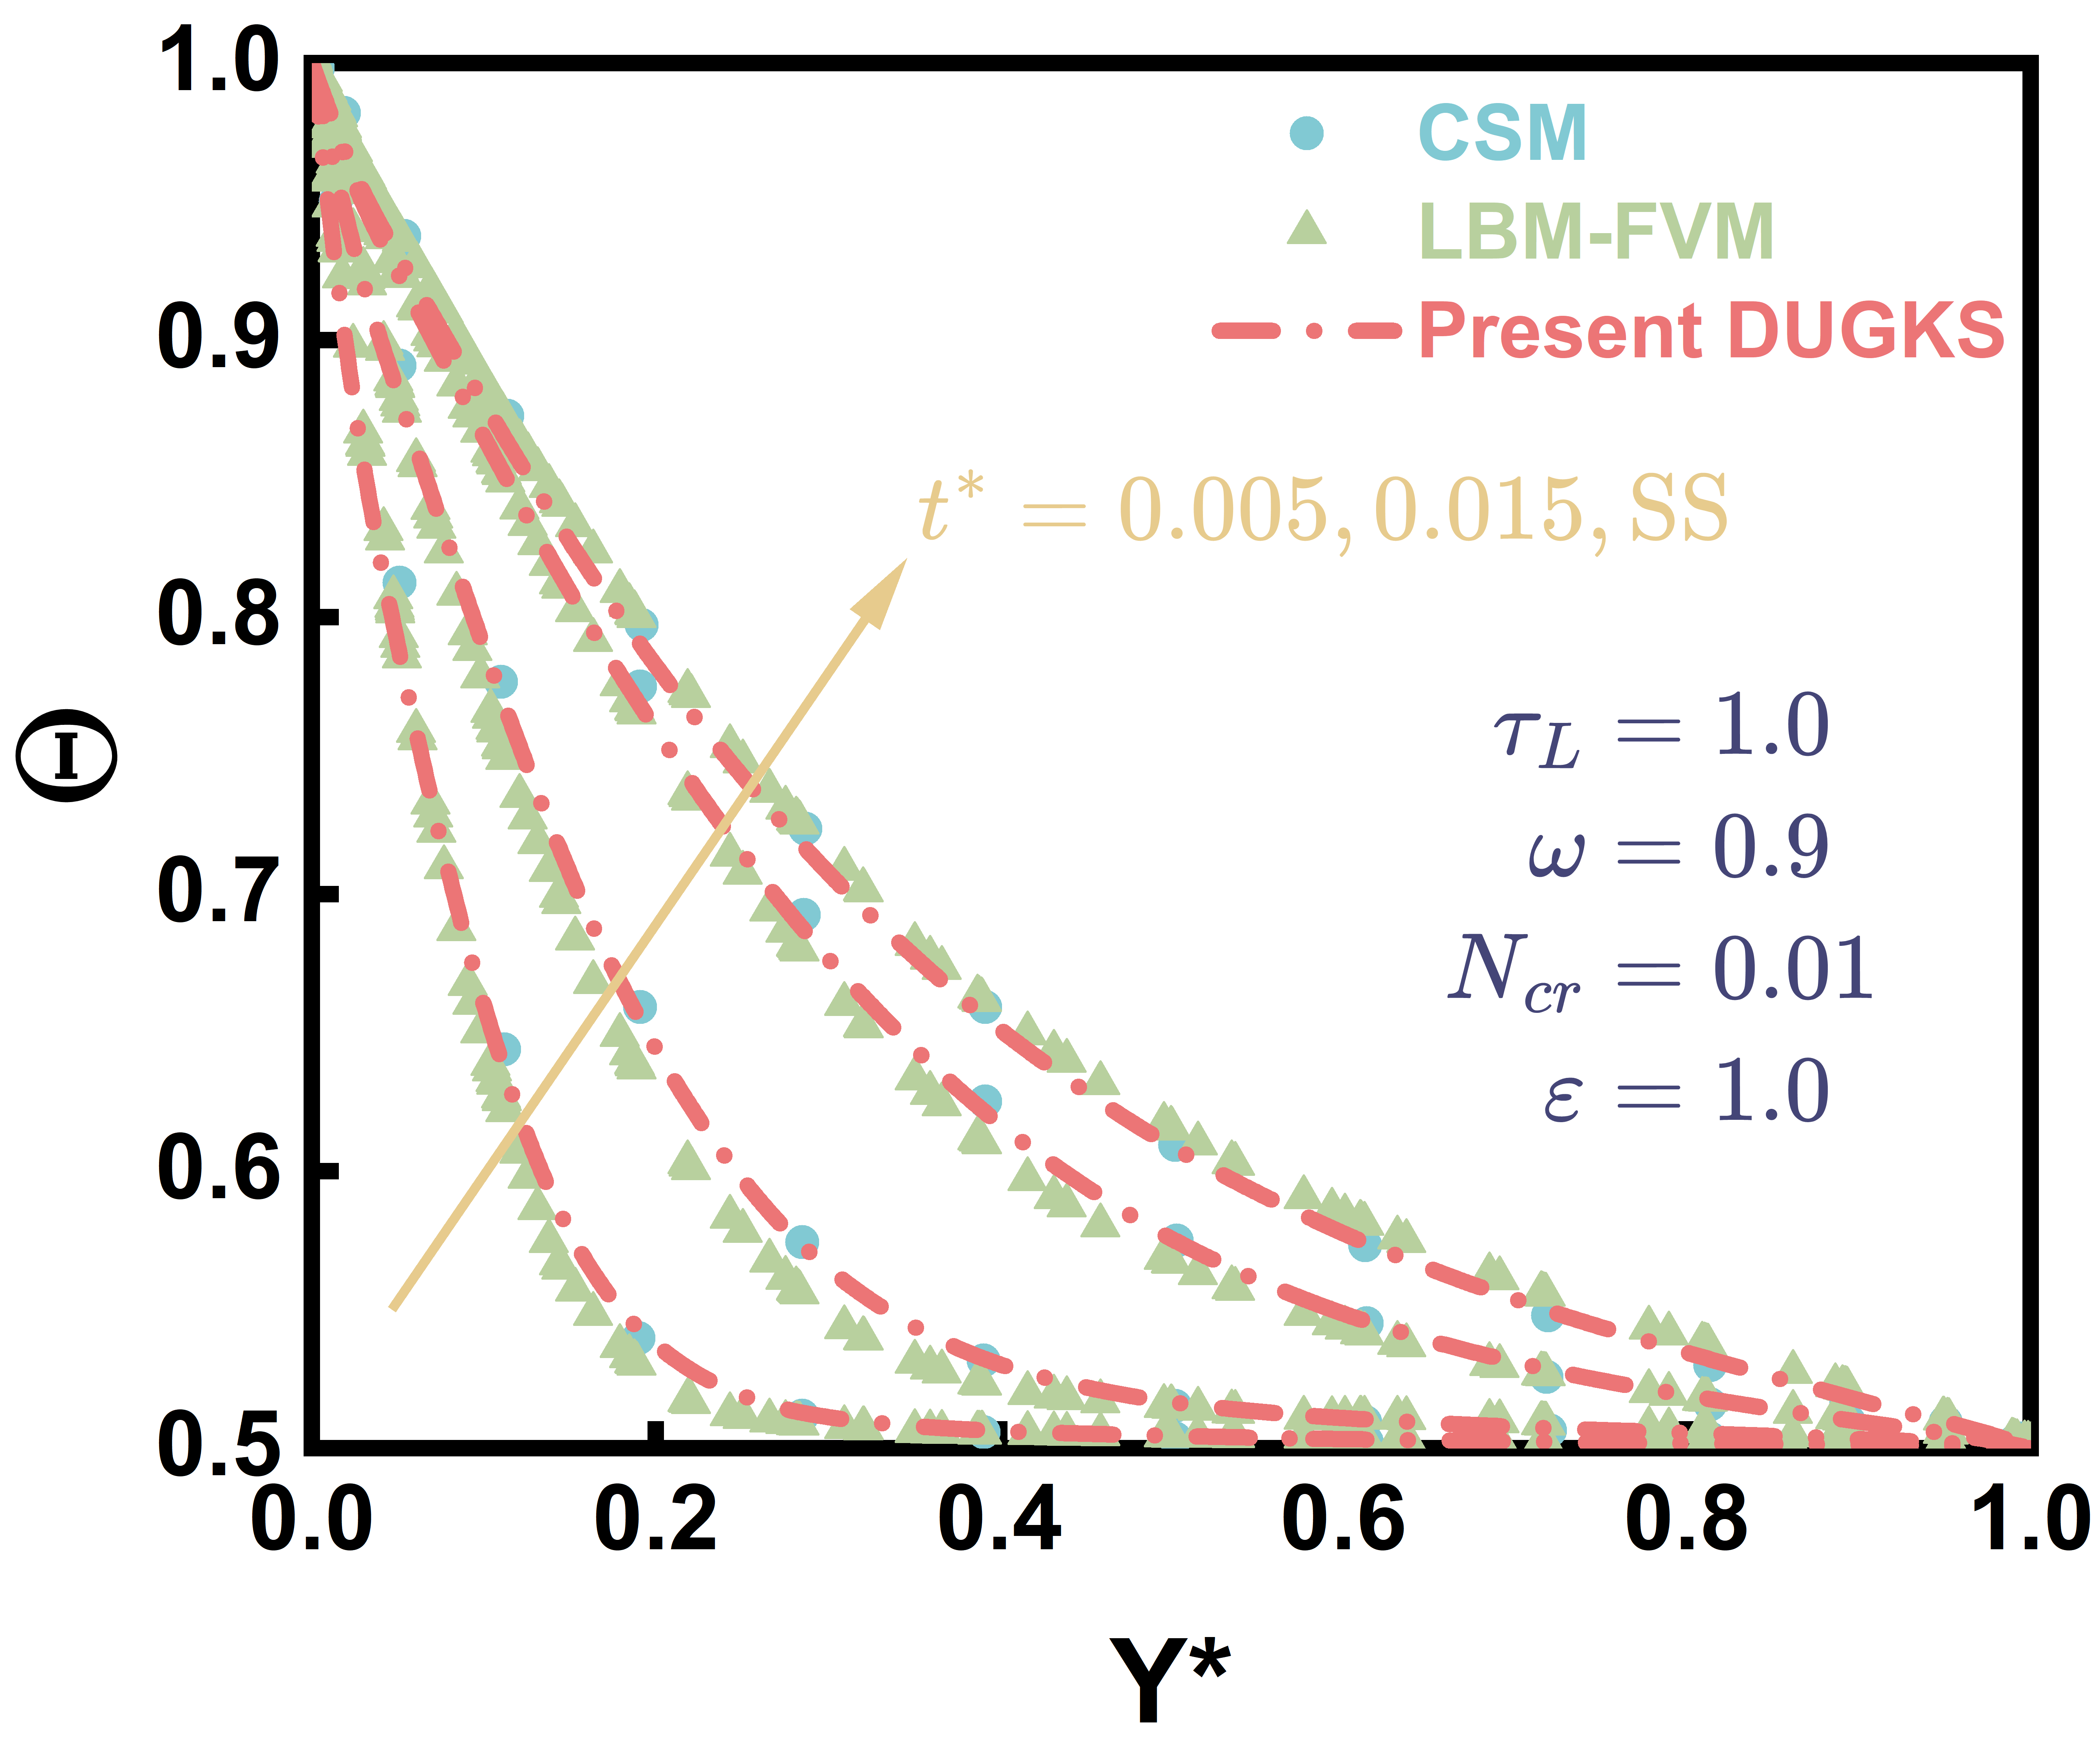
\includegraphics[width=\textwidth]{9B.png}
\caption{}
\end{subfigure}
\caption{Effect of scattering albedo on the centreline temperature in the cubical enclosure. The profiles are taken along $X=0.5$, $Z=0.5$ with $\tau_L=1.0$, $N_{cr}=0.01$, and $\varepsilon=1.0$. Symbols denote the CSM and LBM--FVM reference data reported by Sun et al.~\cite{SunMaLi2012}; dashed lines denote the present DUGKS results.}
\label{fig9}
\end{figure}

\begin{figure}[H]
\centering
\begin{subfigure}[b]{0.48\textwidth}
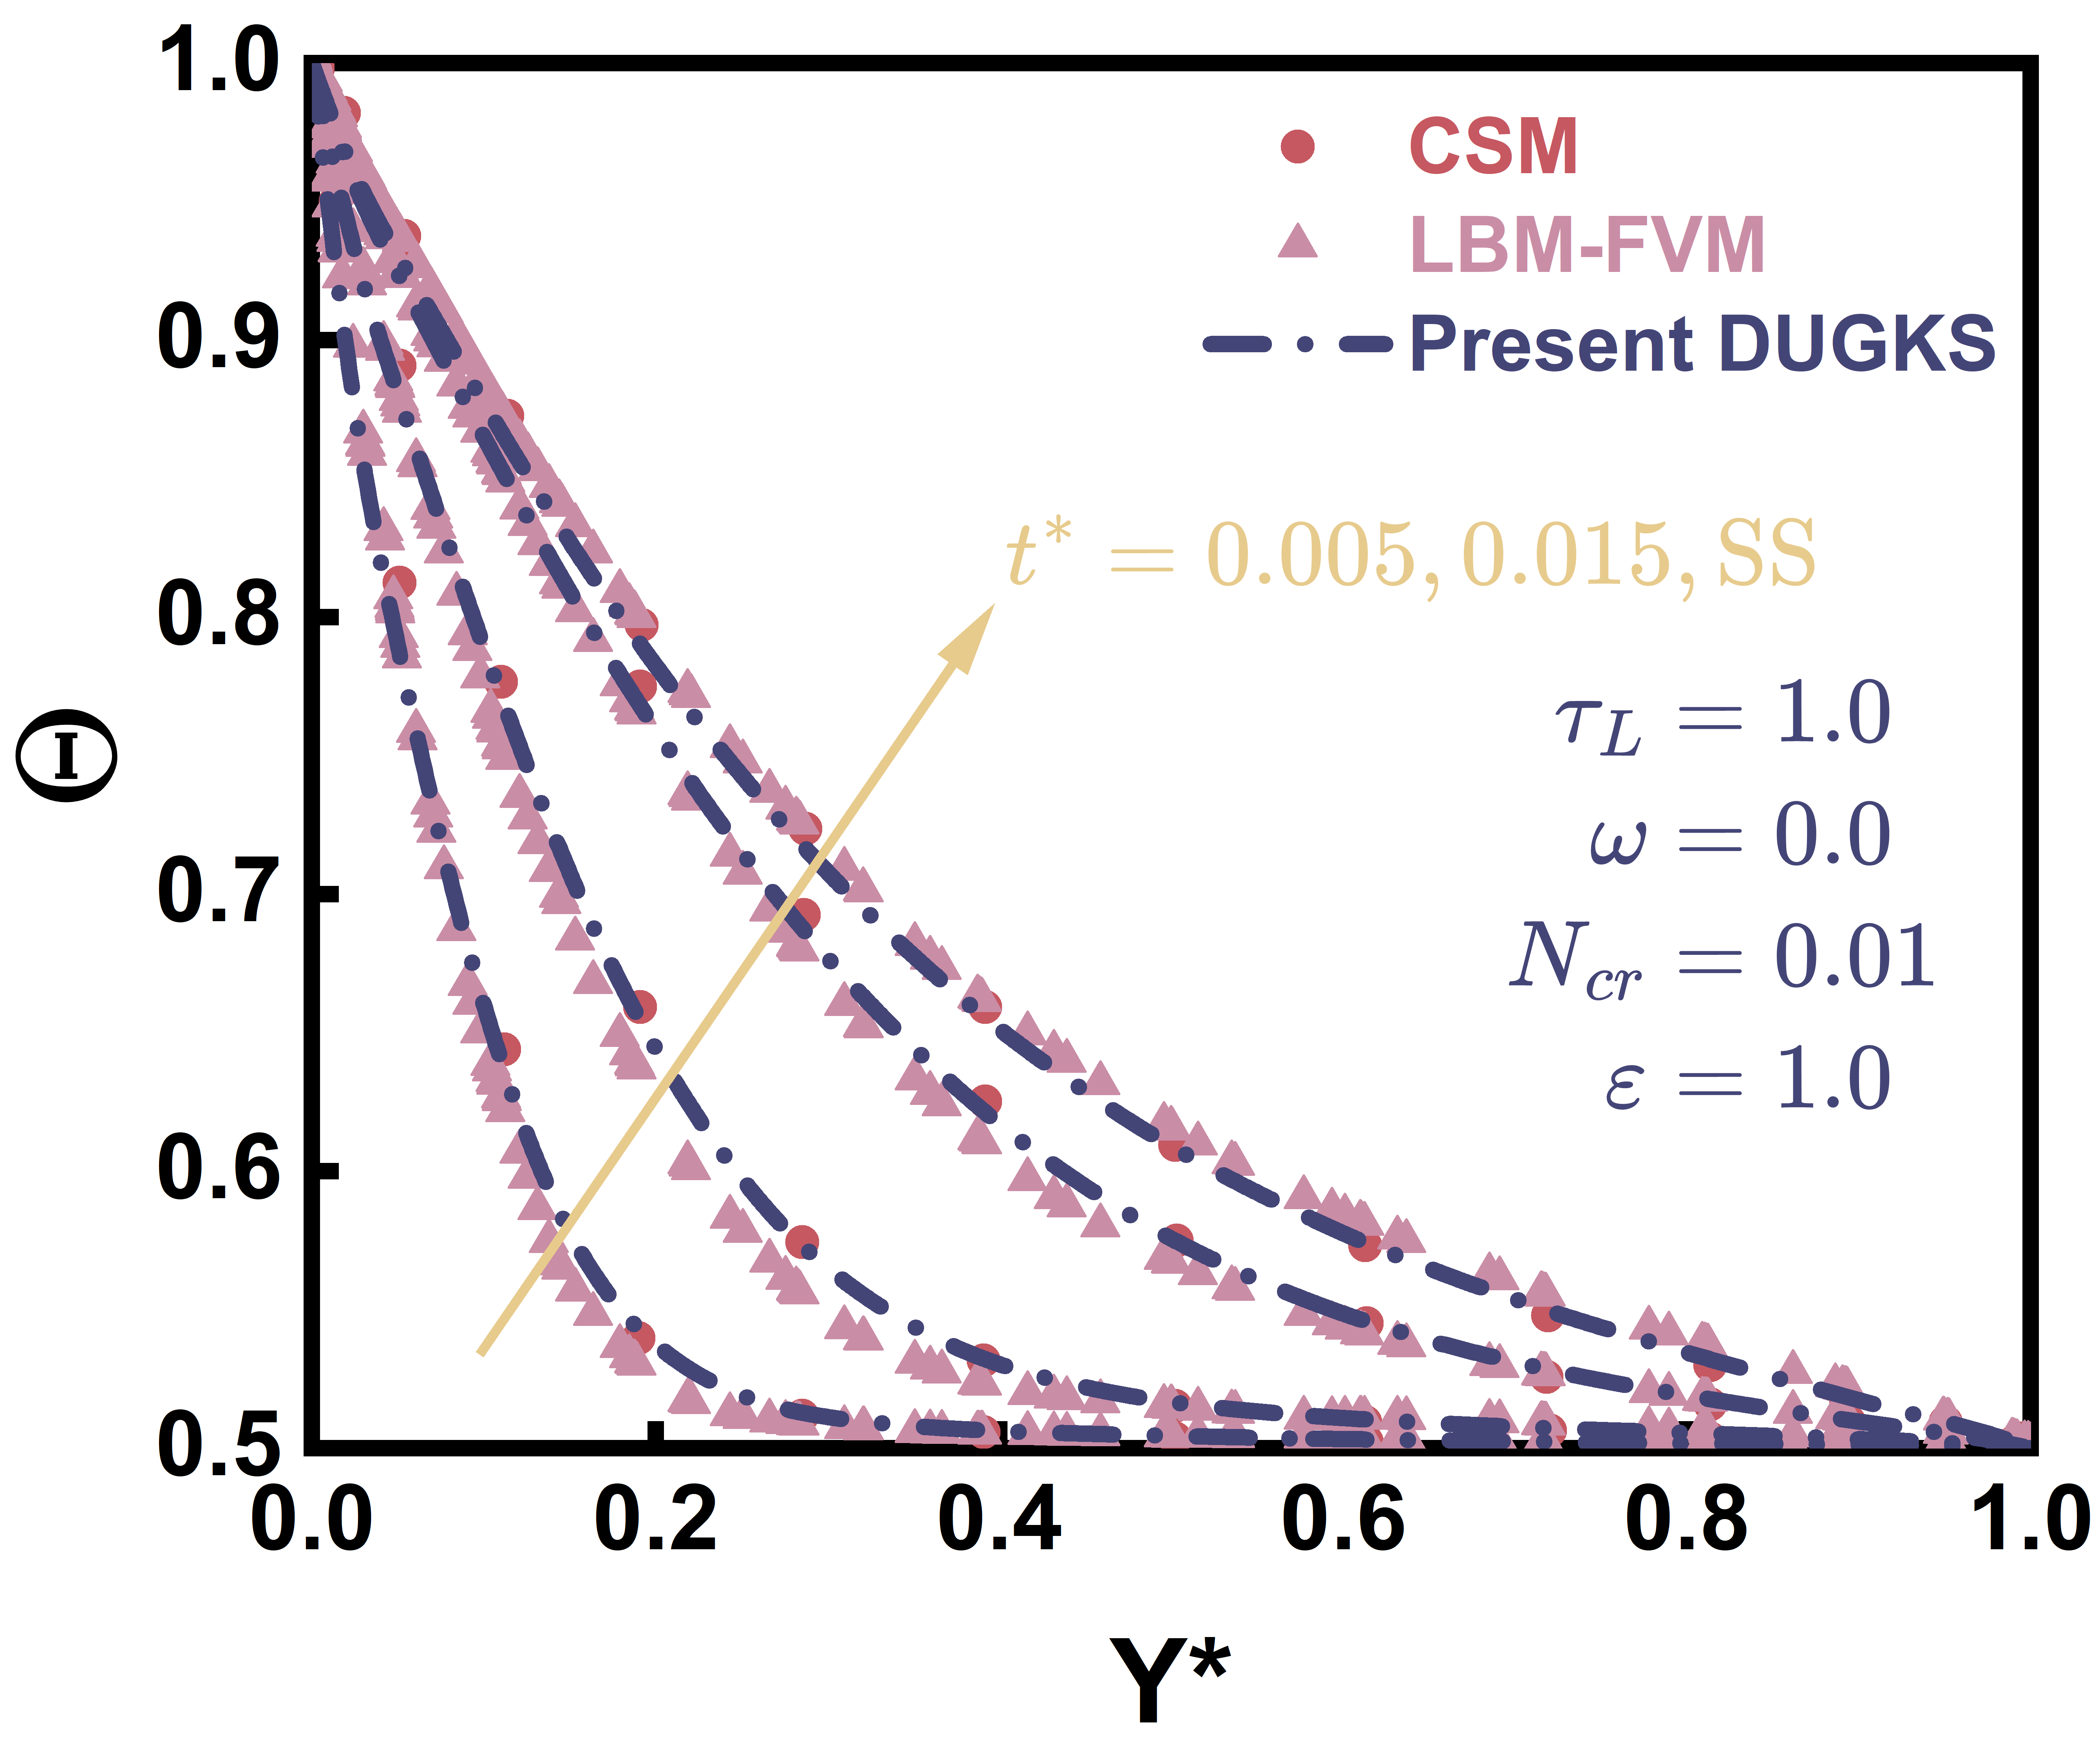
\includegraphics[width=\textwidth]{10A.png}
\caption{}
\end{subfigure}\hfill
\begin{subfigure}[b]{0.48\textwidth}
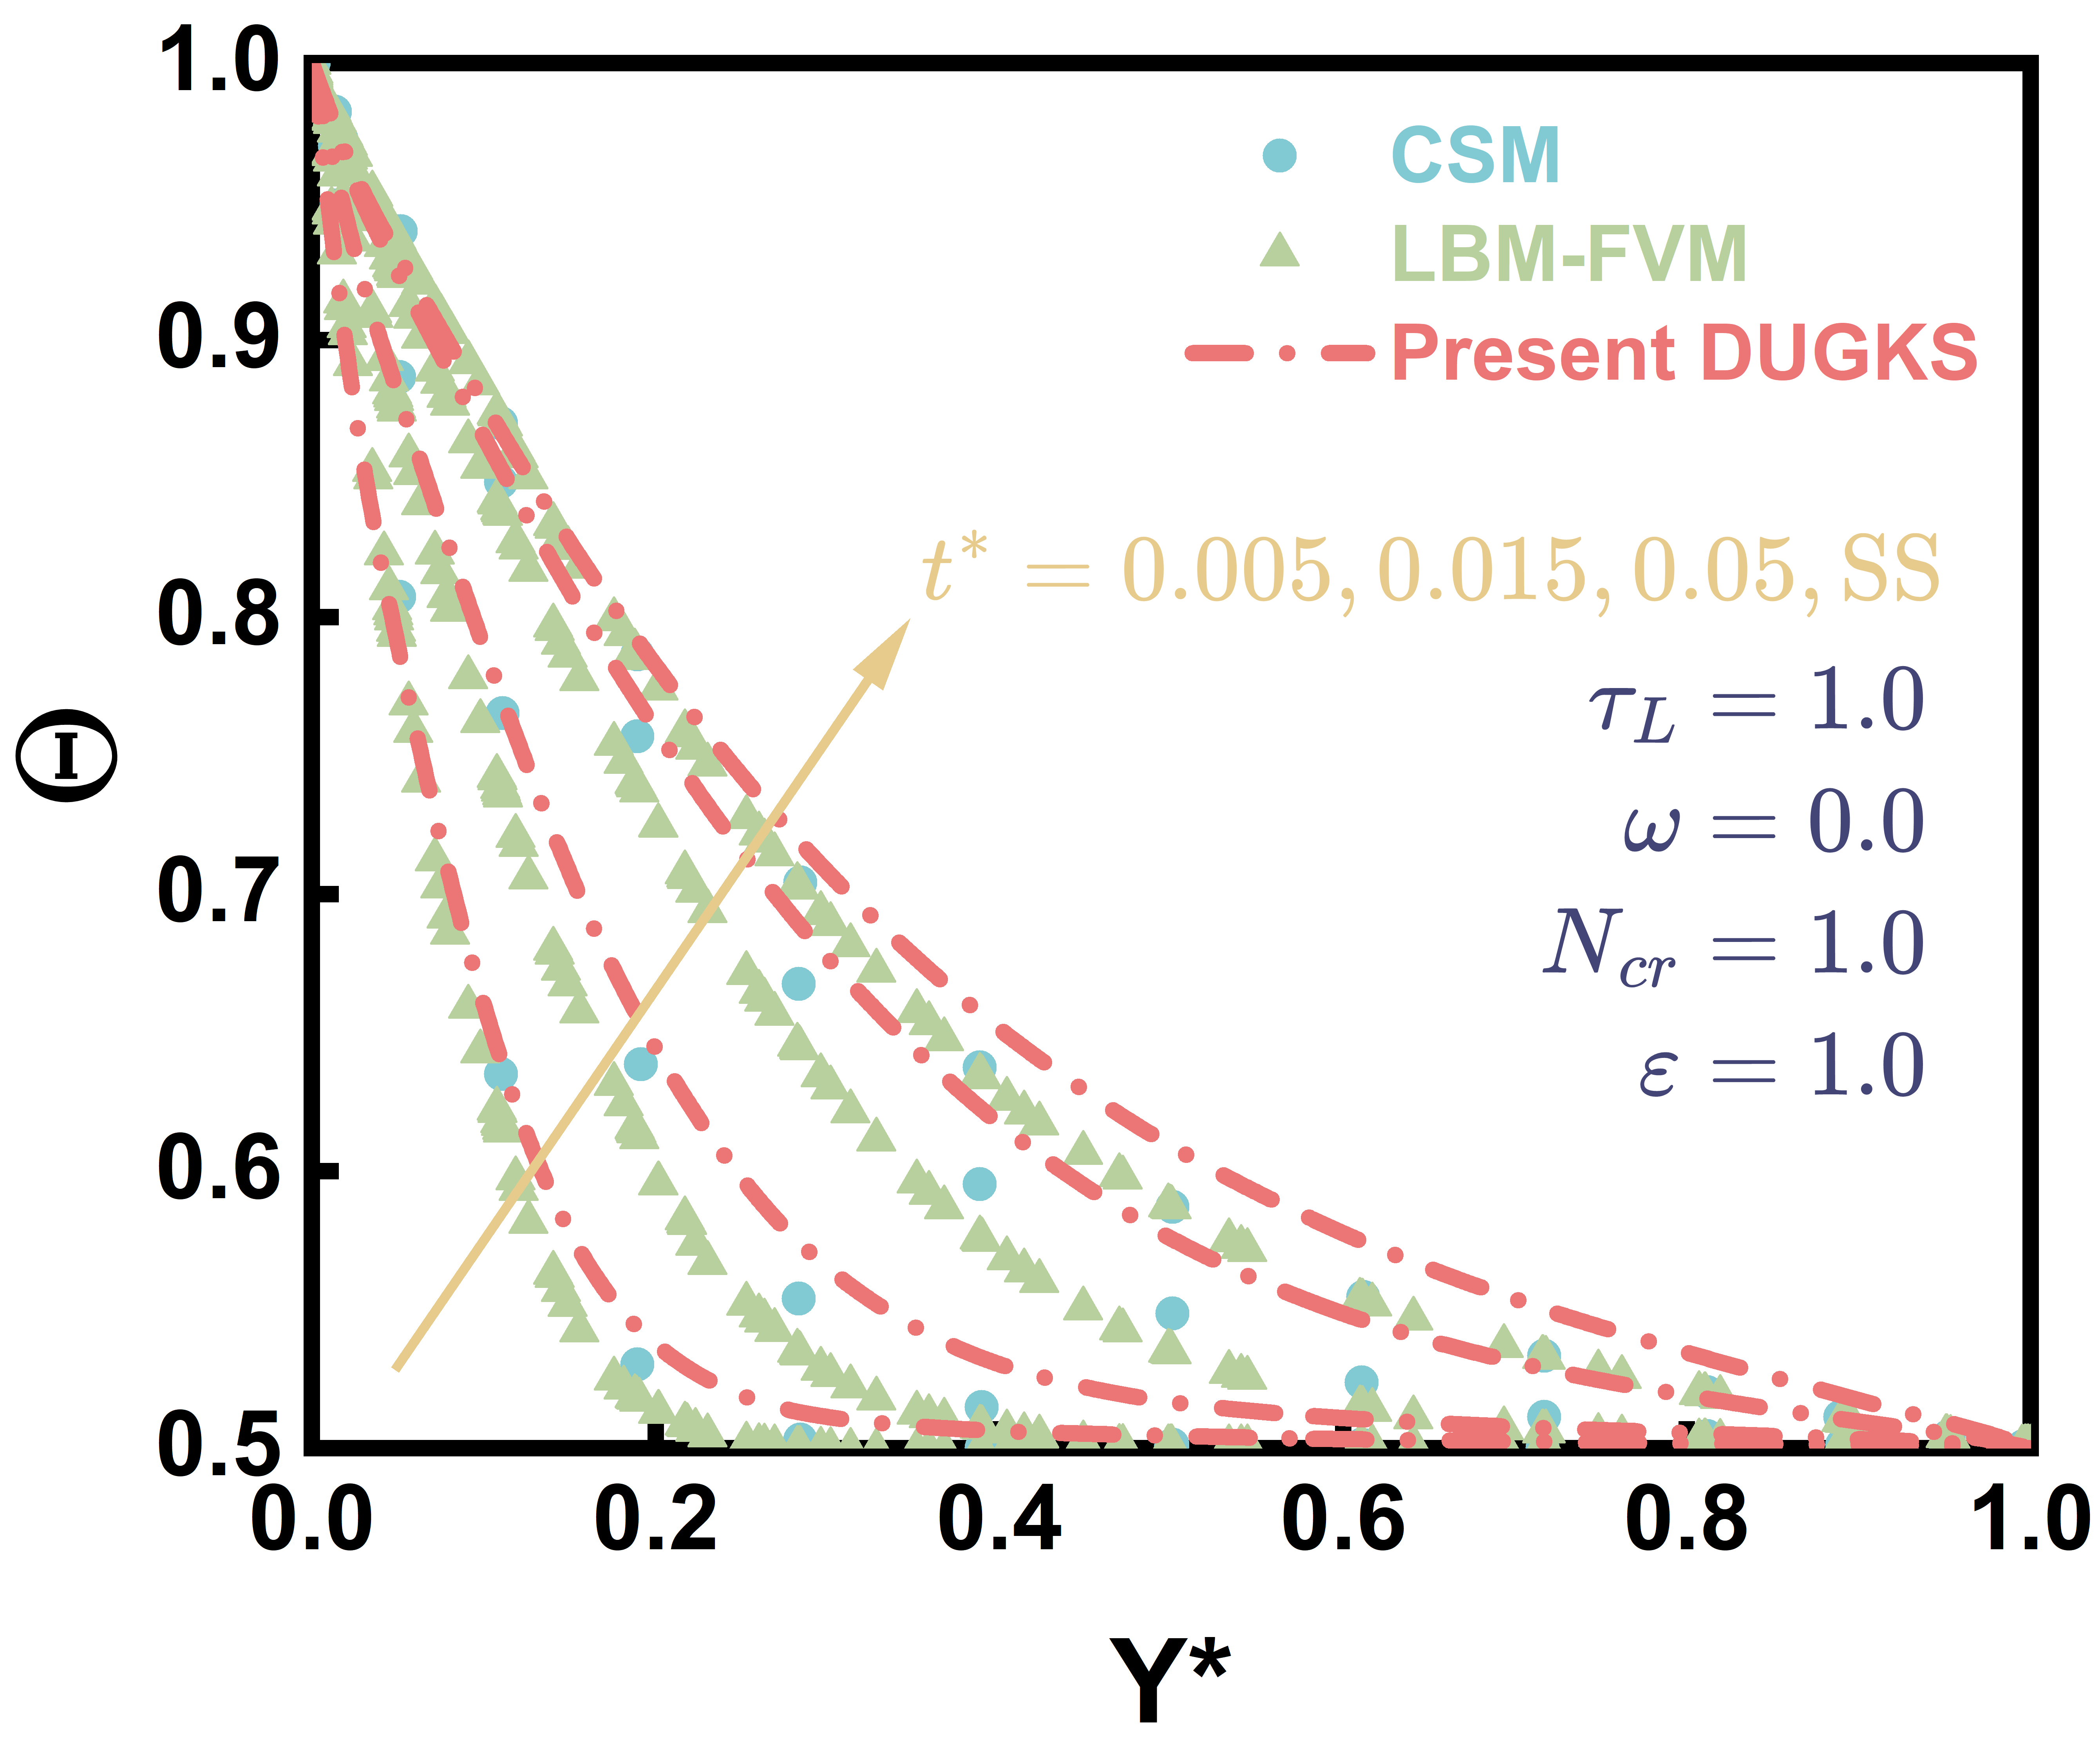
\includegraphics[width=\textwidth]{10B.png}
\caption{}
\end{subfigure}
\caption{Effect of the conduction--radiation parameter on the centreline temperature in the cubical enclosure. The profiles are taken along $X=0.5$, $Z=0.5$ with $\tau_L=1.0$, $\omega=0$, and $\varepsilon=1.0$. Symbols denote the CSM and LBM--FVM reference data reported by Sun et al.~\cite{SunMaLi2012}; dashed lines denote the present DUGKS results.}
\label{fig10}
\end{figure}

\begin{figure}[H]
\centering
\begin{subfigure}[b]{0.48\textwidth}
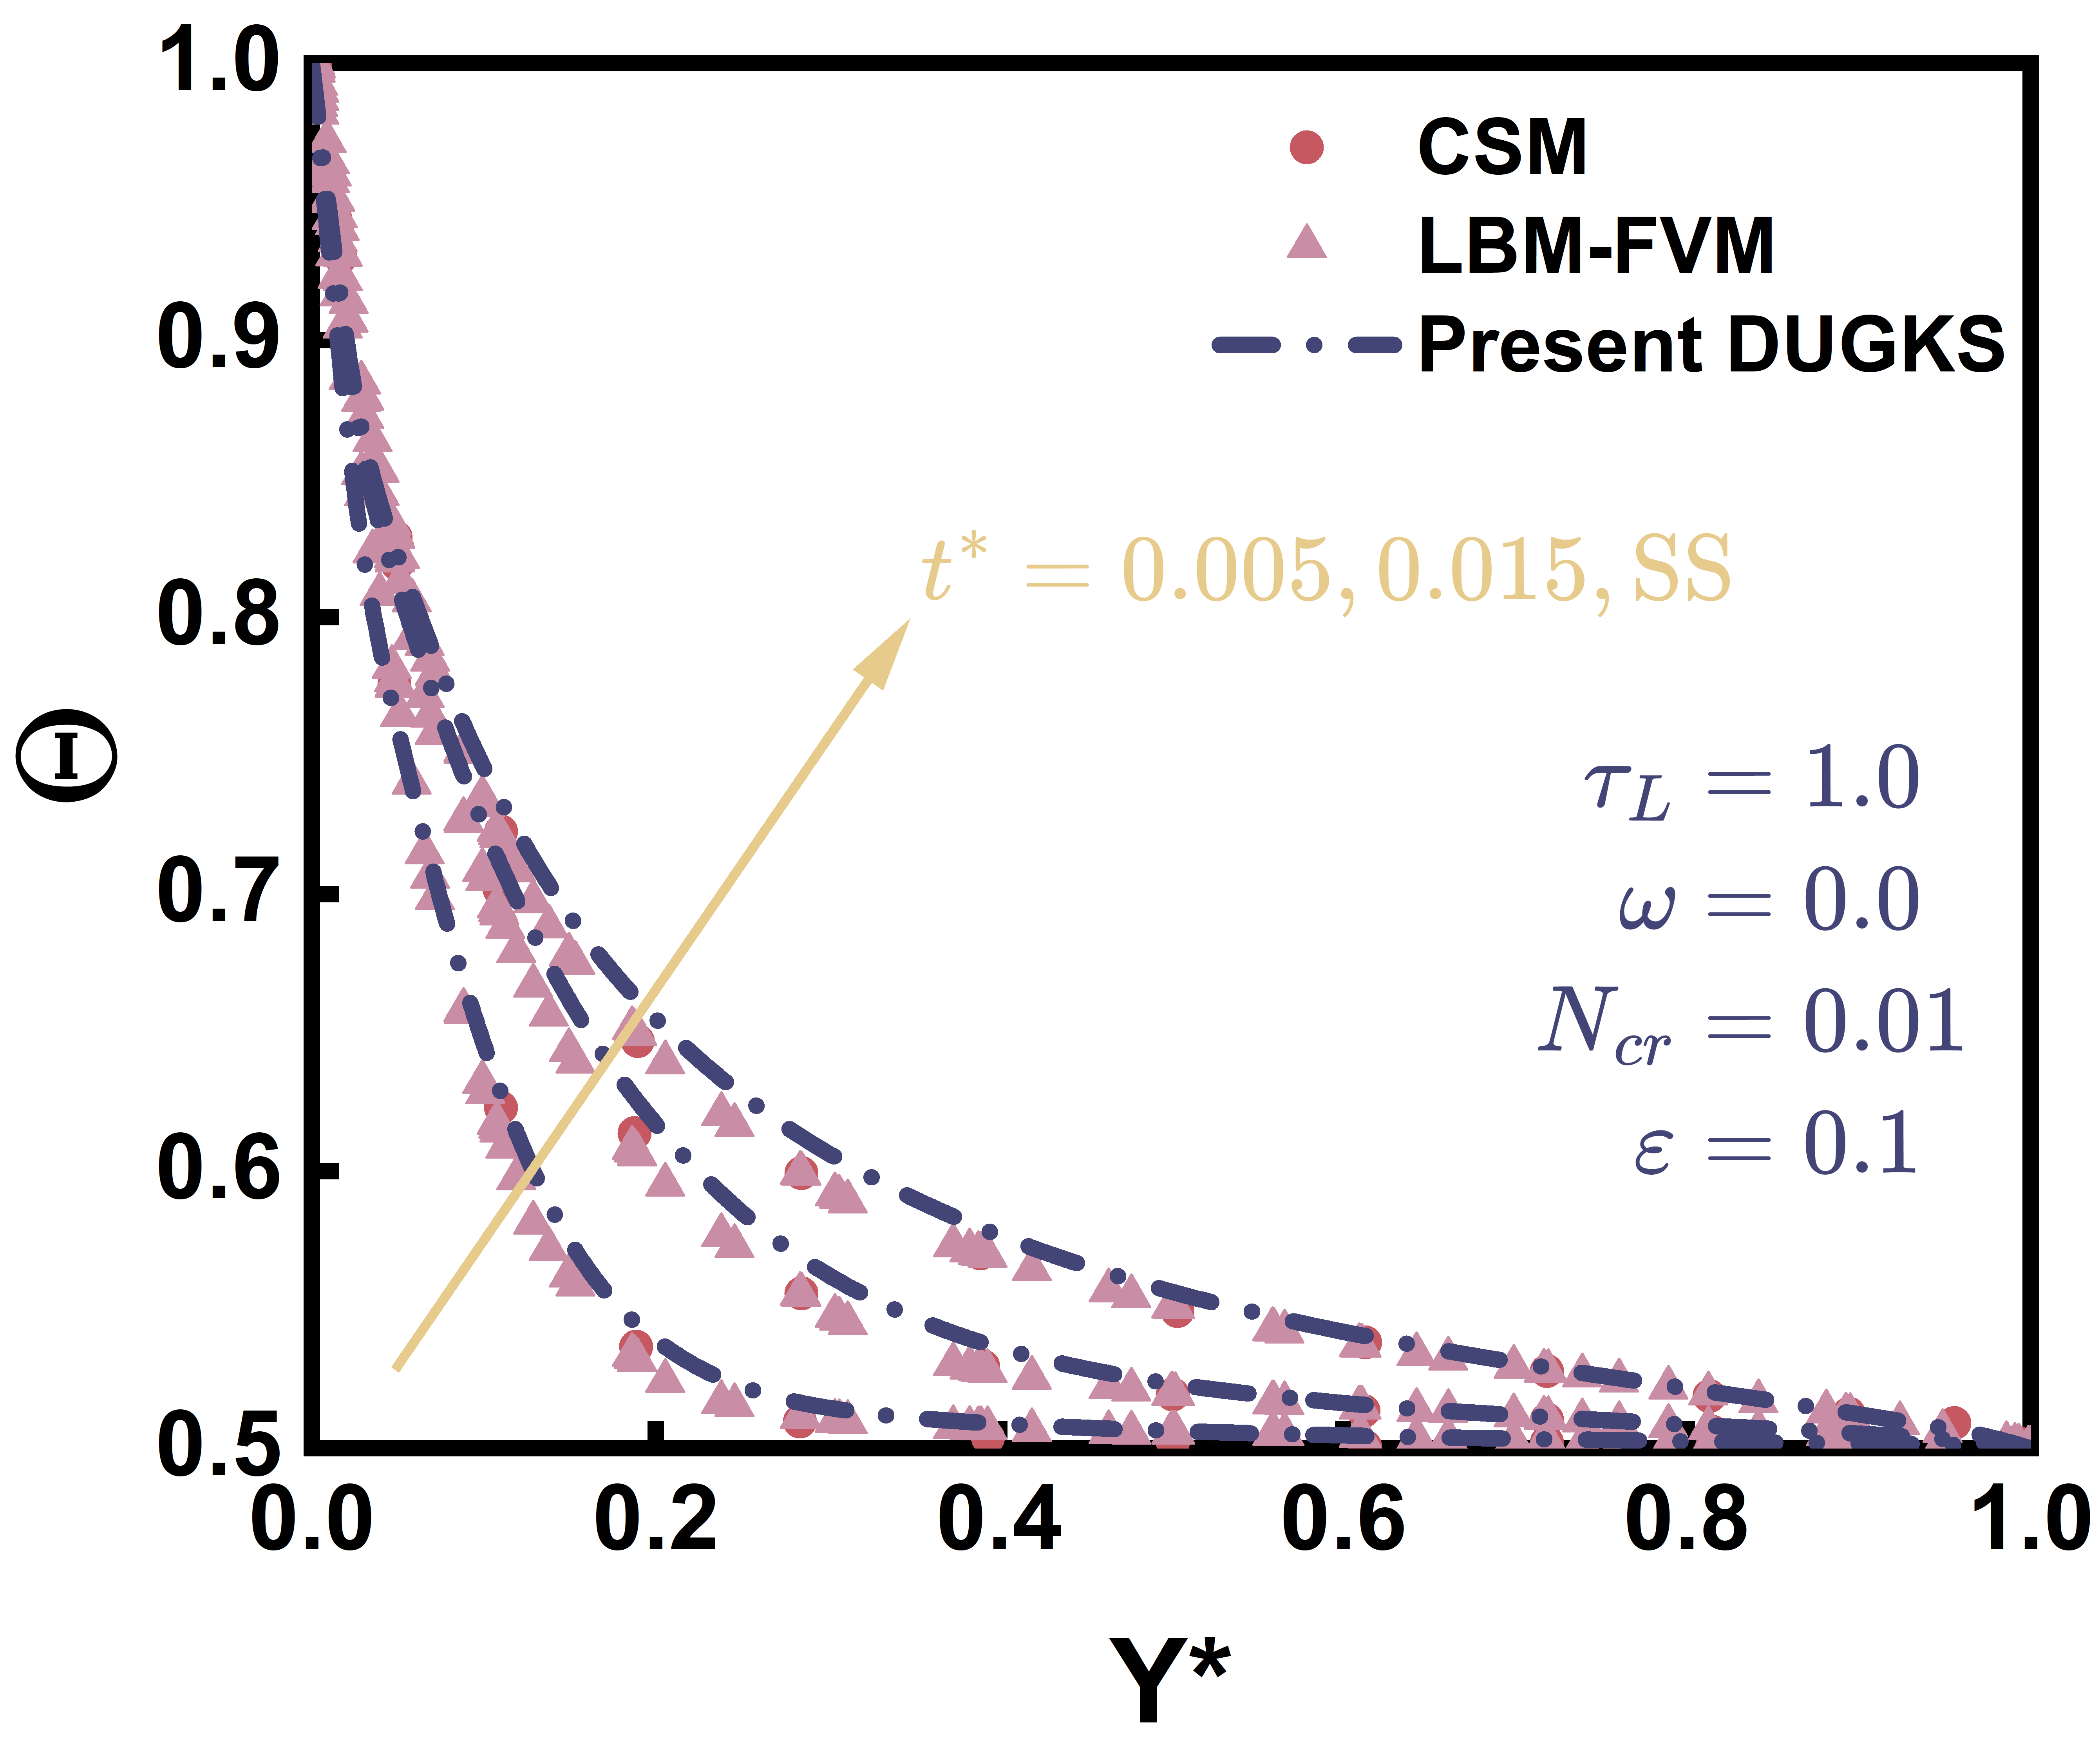
\includegraphics[width=\textwidth]{11A.png}
\caption{}
\end{subfigure}\hfill
\begin{subfigure}[b]{0.48\textwidth}
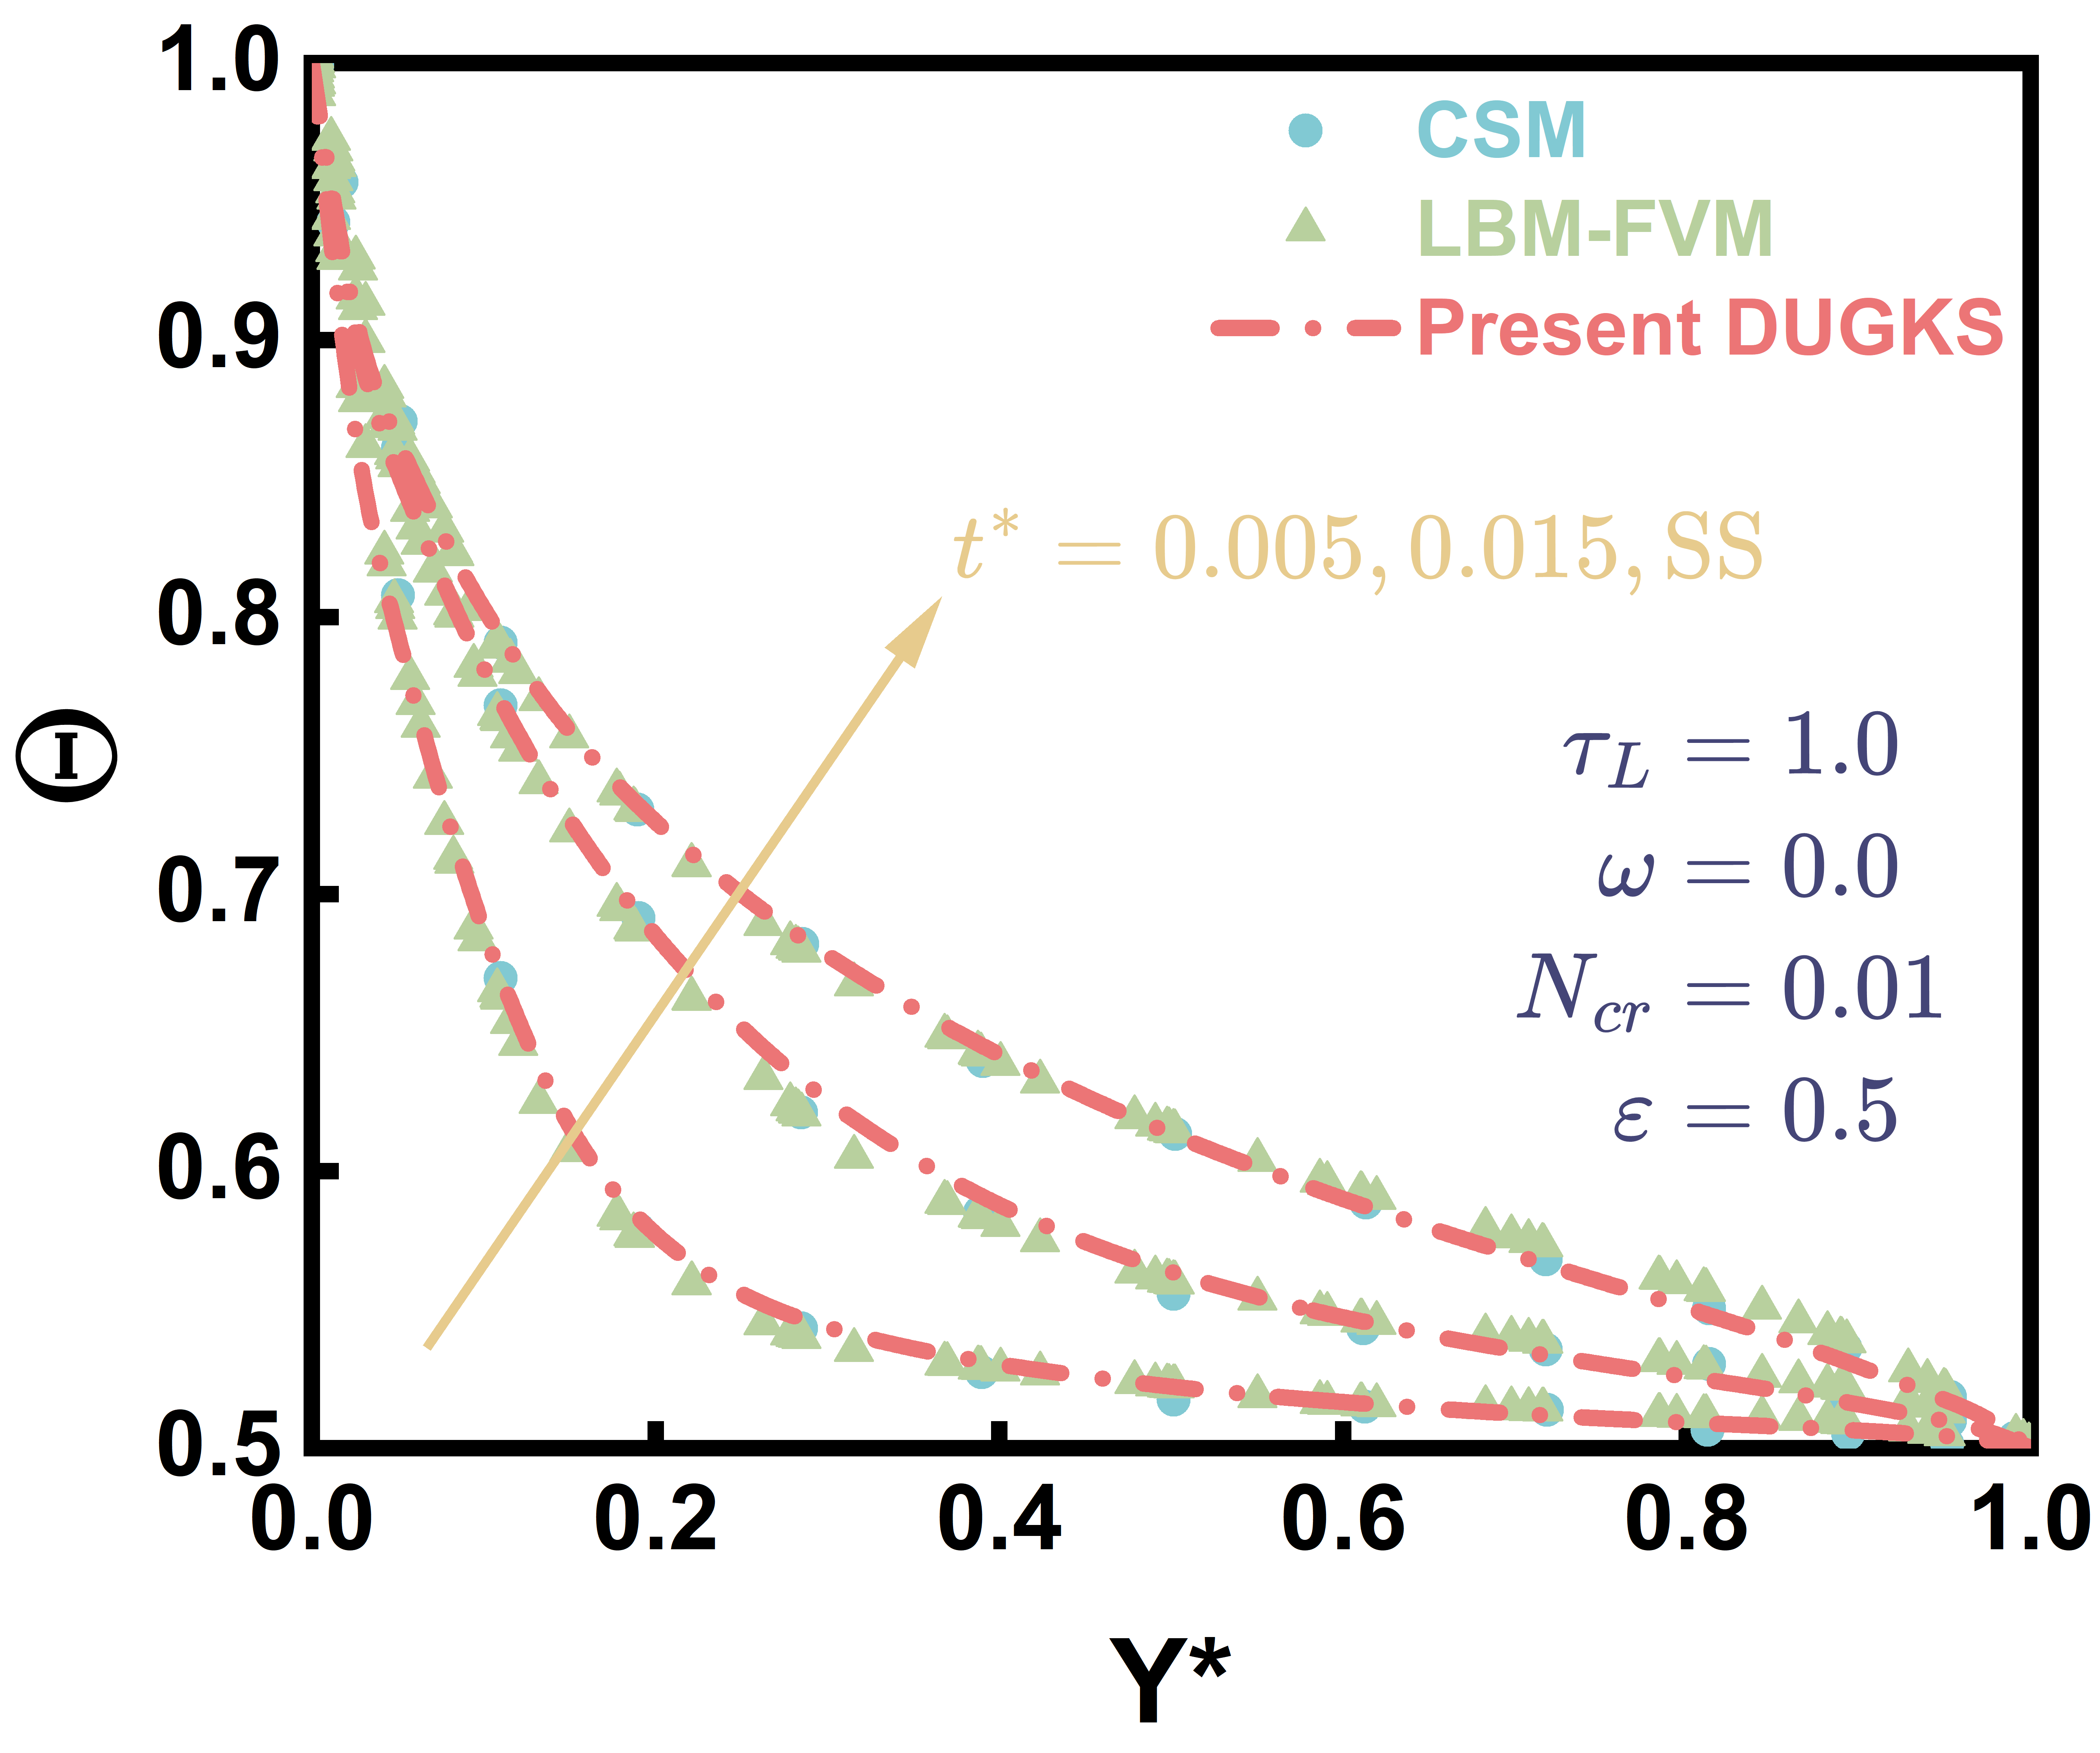
\includegraphics[width=\textwidth]{11B.png}
\caption{}
\end{subfigure}
\caption{Effect of south-wall emissivity on the centreline temperature in the cubical enclosure. The profiles are taken along $X=0.5$, $Z=0.5$ with $\tau_L=1.0$, $\omega=0$, and $N_{cr}=0.01$. Symbols denote the CSM and LBM--FVM reference data reported by Sun et al.~\cite{SunMaLi2012}; dashed lines denote the present DUGKS results.}
\label{fig11}
\end{figure}

\begin{figure}[H]
\centering
\begin{subfigure}[b]{0.48\textwidth}
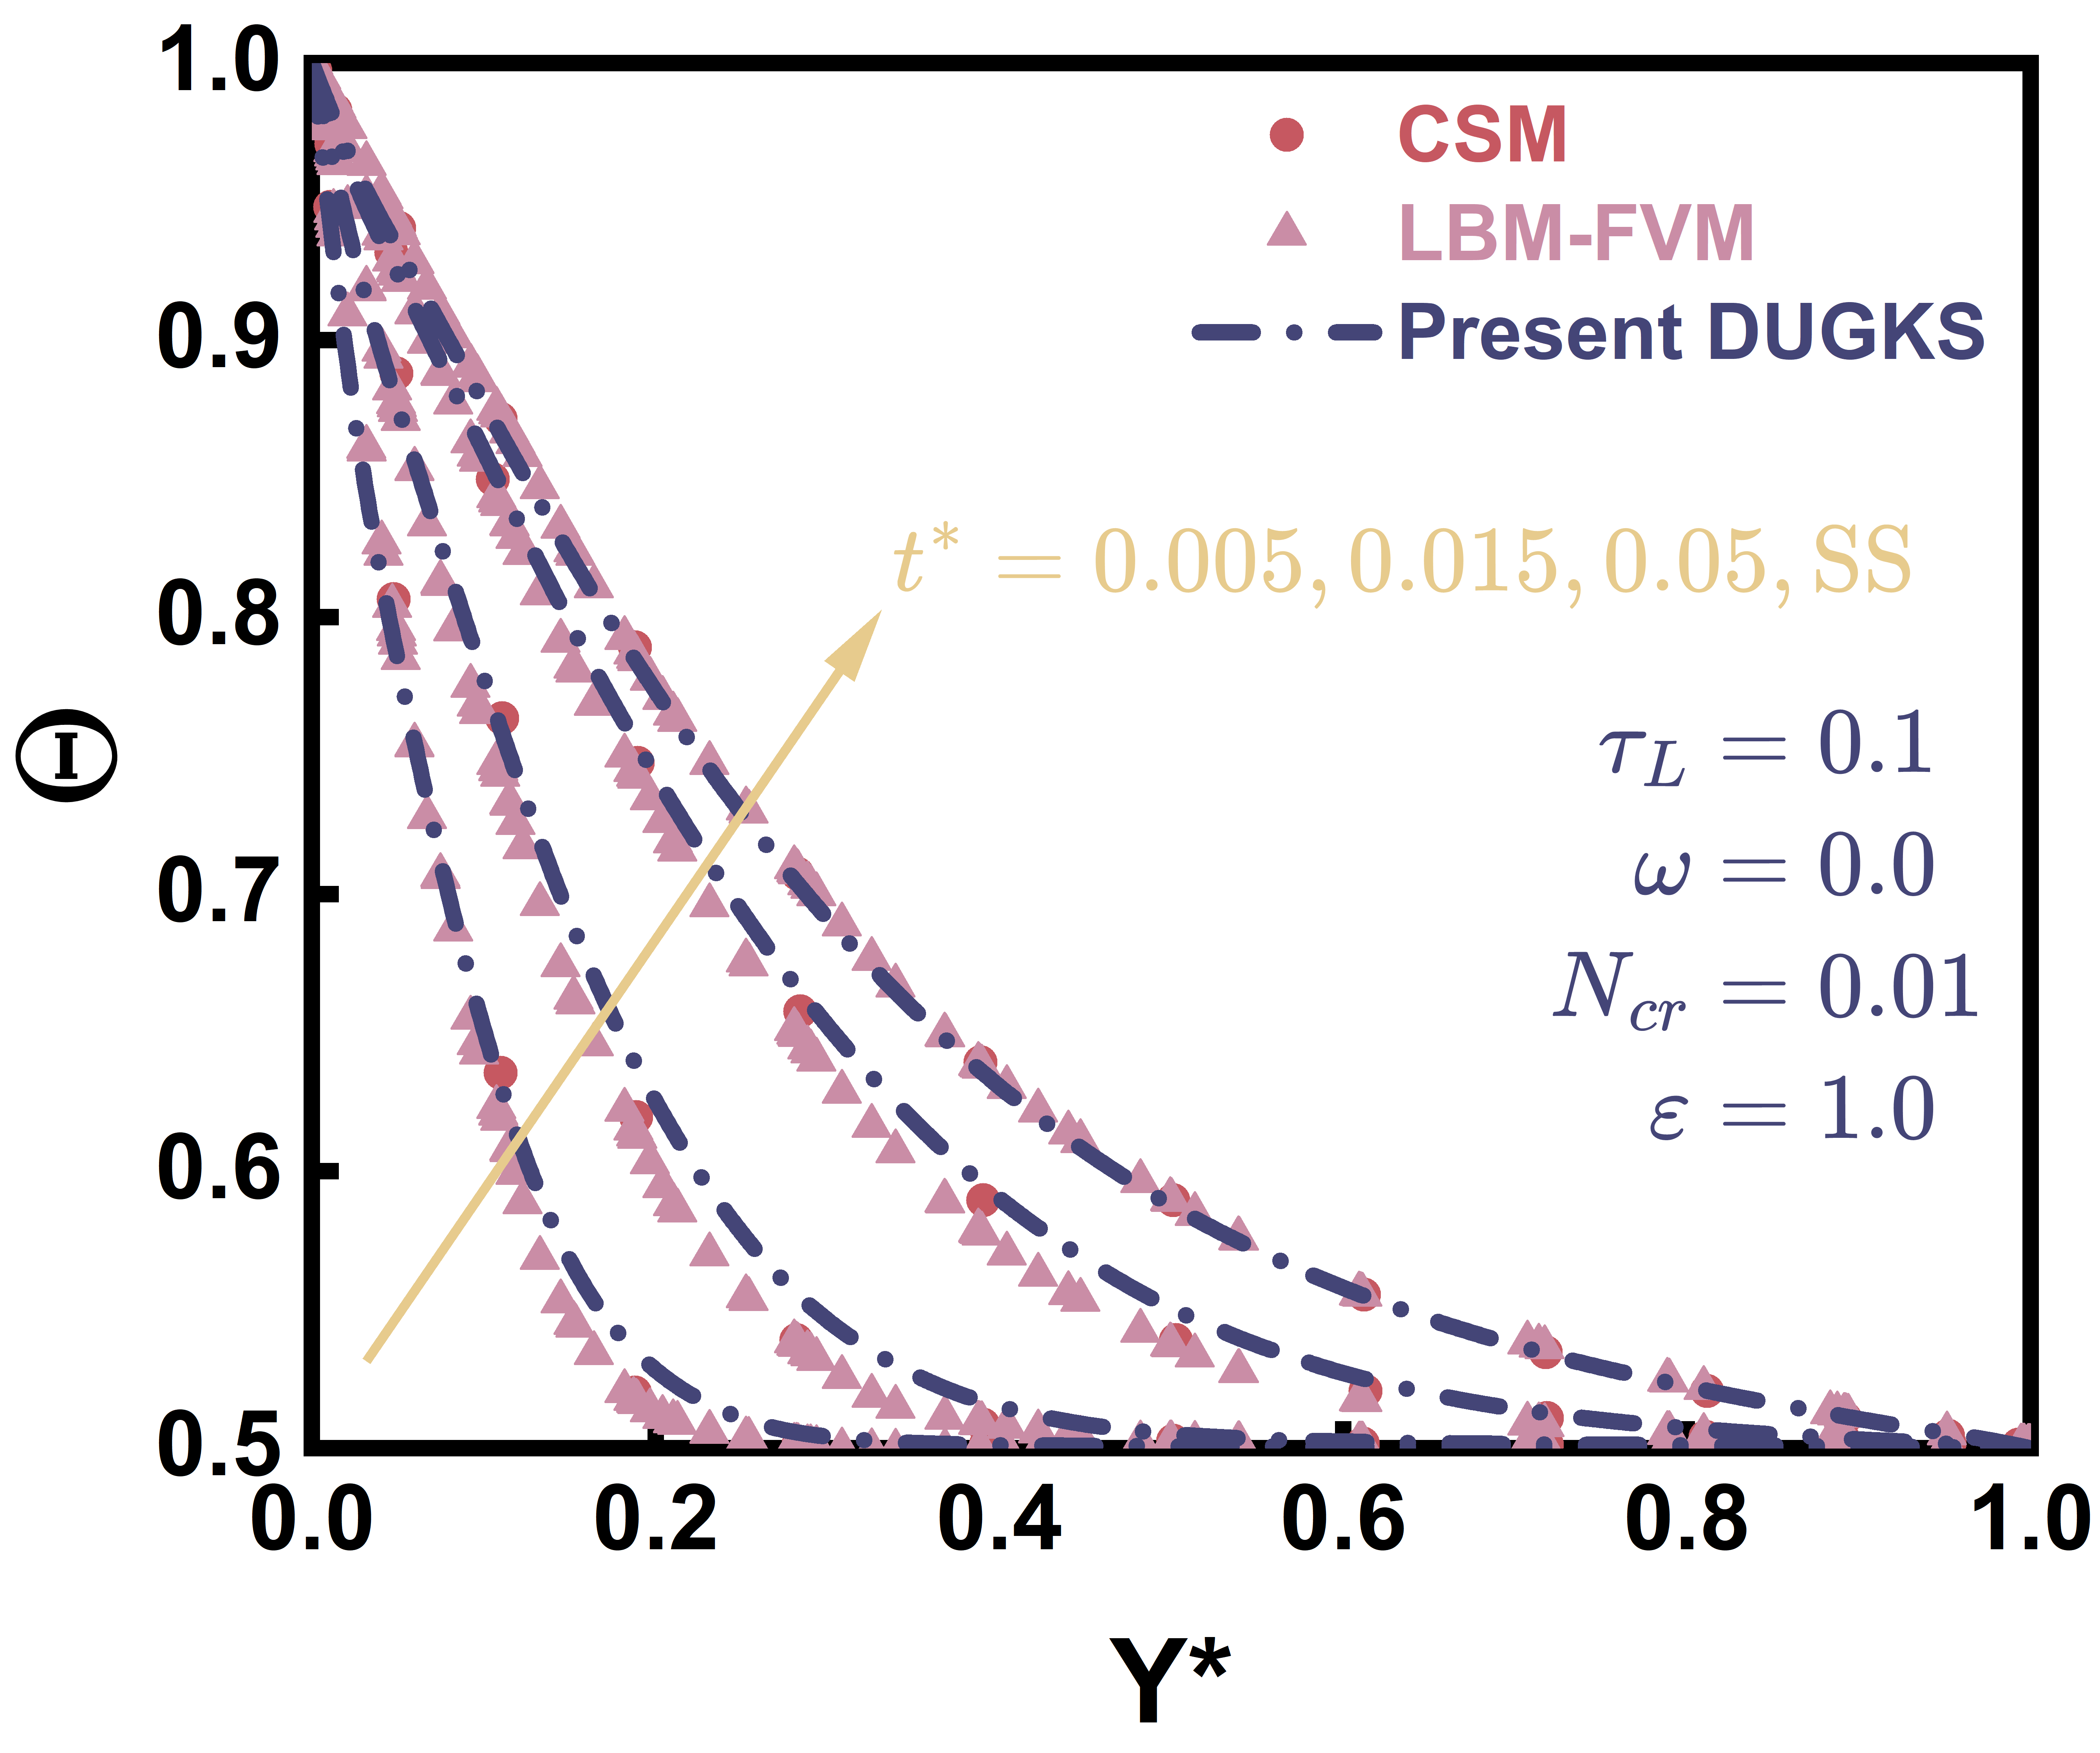
\includegraphics[width=\textwidth]{12A.png}
\caption{}
\end{subfigure}\hfill
\begin{subfigure}[b]{0.48\textwidth}
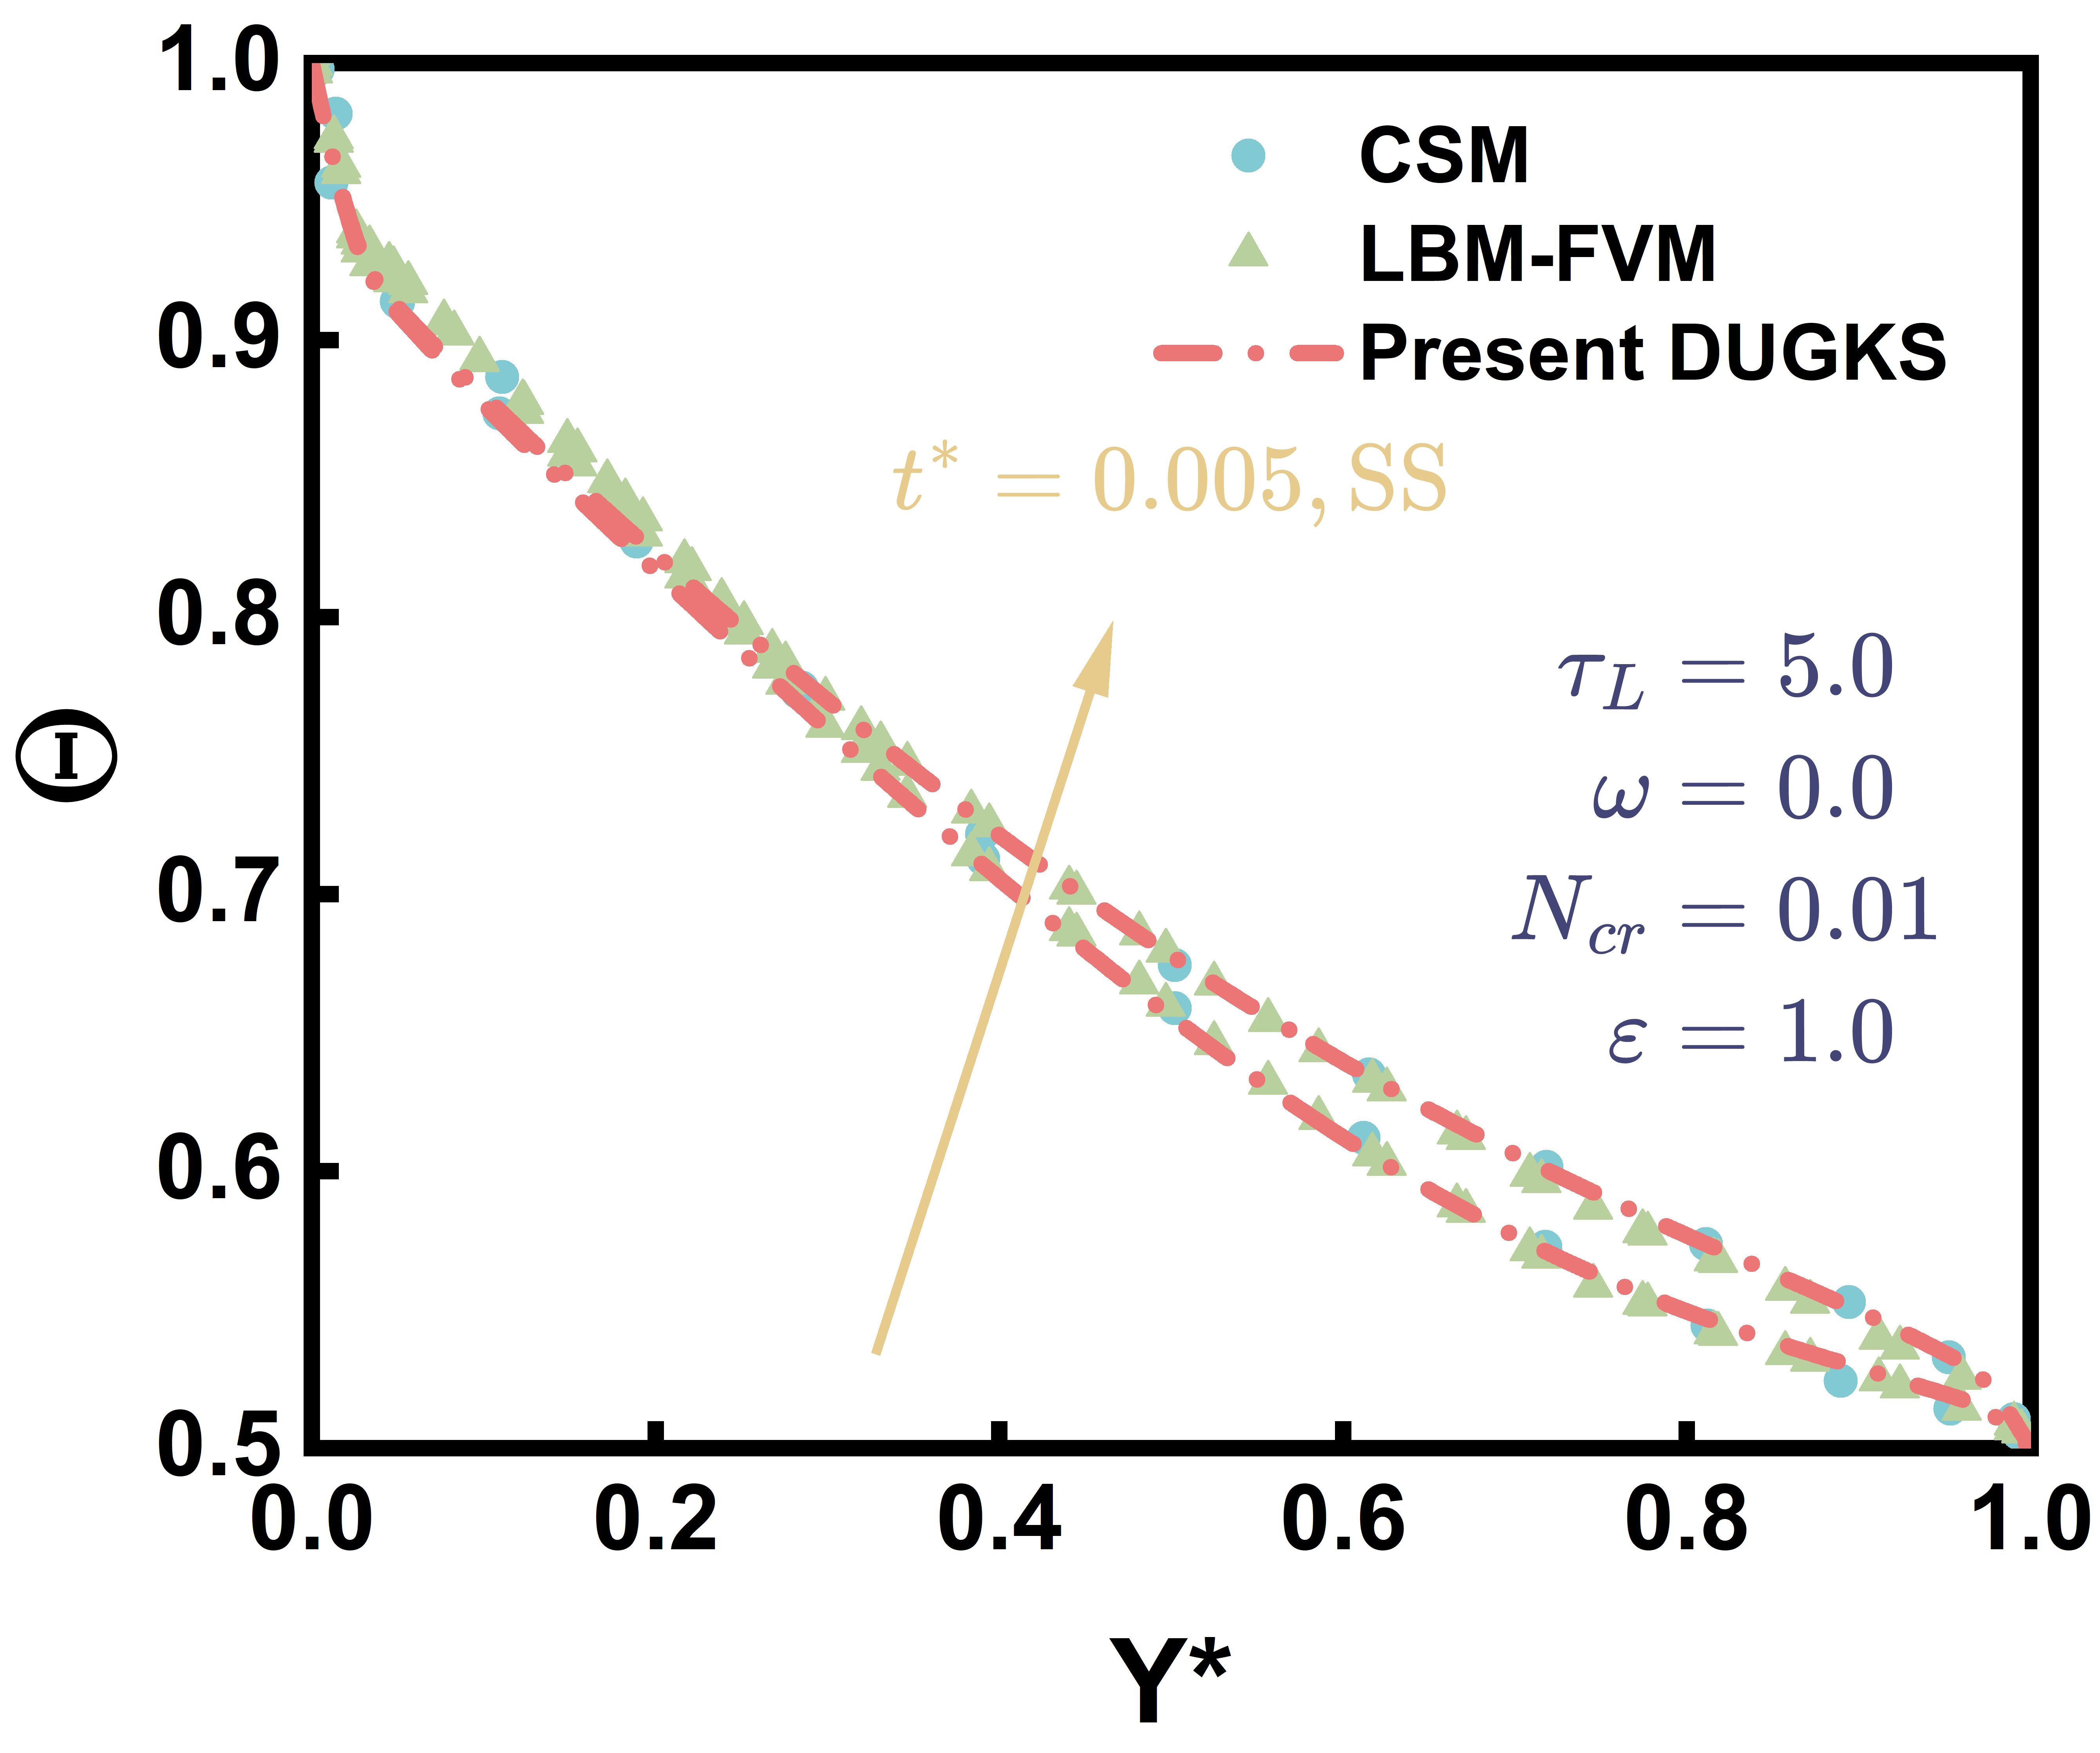
\includegraphics[width=\textwidth]{12B.png}
\caption{}
\end{subfigure}
\caption{Effect of optical thickness on the centreline temperature in the cubical enclosure. The profiles are taken along $X=0.5$, $Z=0.5$ with $\omega=0$, $N_{cr}=0.01$, and $\varepsilon=1.0$. Symbols denote the CSM and LBM--FVM reference data reported by Sun et al.~\cite{SunMaLi2012}; dashed lines denote the present DUGKS results.}
\label{fig12}
\end{figure}

Figures~\ref{fig9}--\ref{fig12} arrange the remaining Sun et al. cubical benchmark conditions in the same order as the original study: scattering albedo, conduction--radiation parameter, south-wall emissivity, and optical thickness. In each case, the plotted curves are centreline temperatures at $X=0.5$ and $Z=0.5$. The present DUGKS profiles follow the reference CSM and LBM--FVM trends over the retained transient times, while the comparison remains a profile-level benchmark check under the single three-dimensional discretisation stated above.

\begin{table}[H]
\centering
\scriptsize
\caption{Representative centre-point temperatures from the current three-dimensional cubical-enclosure calculations. Values are hot-wall-normalised temperatures at $X=0.5$, $Y=0.5$, and $Z=0.5$. The baseline is $\tau_L=1.0$, $\omega=0$, $N_{cr}=0.01$, and $\varepsilon=1.0$. Here, n.r. indicates that the intermediate time was not retained for that run.}
\label{tab:3d_center_values}
\resizebox{\textwidth}{!}{%
\begin{tabular}{@{}l l cccc@{}}
\toprule
Case group & Varied parameter & $t^*=0.005$ & $t^*=0.015$ & $t^*=0.050$ & Steady state \\
\midrule
Baseline transient field & Reference & 0.542 & 0.610 & 0.666 & 0.668 \\
Scattering albedo effect & $\omega=0.5$ & 0.528 & 0.577 & n.r. & 0.659 \\
Scattering albedo effect & $\omega=0.9$ & 0.507 & 0.524 & 0.588 & 0.619 \\
Conduction--radiation parameter effect & $N_{cr}=0.1$ & 0.504 & 0.517 & 0.576 & 0.609 \\
Conduction--radiation parameter effect & $N_{cr}=1.0$ & 0.500 & 0.504 & 0.549 & 0.586 \\
South-wall emissivity effect & $\varepsilon_S=0.1$ & 0.506 & 0.523 & n.r. & 0.556 \\
South-wall emissivity effect & $\varepsilon_S=0.5$ & 0.522 & 0.564 & n.r. & 0.613 \\
Optical-thickness effect & $\tau_L=0.1$ & 0.501 & 0.505 & 0.550 & 0.587 \\
Optical-thickness effect & $\tau_L=5.0$ & 0.656 & n.r. & n.r. & 0.678 \\
\bottomrule
\end{tabular}%
}
\end{table}

The centre-point values in Table~\ref{tab:3d_center_values} quantify the trends visible in Figs.~\ref{fig9}--\ref{fig12}. At fixed $\tau_L$ and $N_{cr}$, increasing the scattering albedo from $\omega=0.5$ to $0.9$ lowered the centre-point steady temperature from $0.659$ to $0.619$, which is consistent with weaker conversion of radiative transport into material heating. Increasing $N_{cr}$ from $0.1$ to $1.0$ also lowered the centre-point steady temperature, from $0.609$ to $0.586$, because the radiative source is reduced relative to conduction. Boundary emission produced a separate control: the steady centre-point temperature was $0.556$ at $\varepsilon_S=0.1$ and $0.613$ at $\varepsilon_S=0.5$. The optical-thickness sweep changed both the radiative propagation scale and the thermal diffusion coefficient in Eq.~\eqref{eq:3d_energy_sun}; the centre point therefore remained close to its initial value for $\tau_L=0.1$ at early time but warmed rapidly for $\tau_L=5.0$.

This subsection therefore completes the bridge from the existing one- and two-dimensional benchmark comparisons to the fully three-dimensional case. The current cubical results use the same temperature and radiation solvers as the lower-dimensional benchmarks; no additional governing equation or interpolation procedure is required. A separate grid and angular-independence study is still needed before the three-dimensional curves are used as final quantitative benchmark data.

\section{Discussion}
\label{sec:discussion}

The results support two bounded numerical claims. First, the coupled DUGKS reproduces established transient conduction--radiation benchmarks in planar and square media. It recovered the nonlinear temperature and decomposed heat-flux behaviour reported for the one-dimensional slab~\cite{Talukdar2001}, and it reproduced the centreline behaviour of the two-dimensional LBM--FVM benchmark~\cite{Sun2016}. Second, the same update structure can be applied to the cubical benchmark without introducing a separate radiation mesh. In that case, the calculation must treat three coordinate fluxes, six wall boundaries, and optical-thickness-scaled radiative transport.

The principal numerical contribution is the shared DUGKS update used for conduction and radiation. A kinetic representation advances temperature, while pseudo-time relaxation resolves the angular intensity. Both equations use characteristic interface reconstruction on the same control-volume grid. The radiative source is therefore evaluated directly at temperature nodes without inter-mesh interpolation. This alignment matters because $G$ and the nonlinear emission term $\theta^4$ are updated during every physical time step.

The parametric trends reflect distinct controls on energy exchange. Increasing scattering albedo redirects more radiation without converting it into material energy, which weakens volumetric heating. Increasing $N$ or $N_{cr}$ reduces the radiative source relative to thermal diffusion, so the response approaches a conduction-dominated limit. Reducing wall emissivity lowers emitted radiation at the heated boundary and delays interior warming. The optical-thickness sweep further shows that three-dimensional transport cannot be inferred only from the unit-optical-thickness case, because $\tau_L$ changes both radiative propagation and thermal diffusion scaling in the cubical formulation.

Angular convergence depended on the reported quantity in the two-dimensional tests. Temperature changed little beyond $N_\phi=8$, whereas heat flux retained visible angular-discretisation errors. This difference arises because radiative heat flux is the first angular moment of intensity. Flux prediction therefore requires a finer representation of directionality than temperature prediction. The current three-dimensional calculations used $N_\theta=8$ and $N_\phi=16$ as the principal angular set, but a dedicated three-dimensional angular sweep remains necessary for final quantitative validation.

The present evidence is bounded by the benchmark assumptions. The calculations considered gray media, isotropic scattering, constant properties, and regular slab, square, or cubical geometries. They do not establish performance for non-gray radiation, anisotropic scattering, strongly temperature-dependent properties, or complex boundaries. The present benchmarks also do not by themselves prove formal accuracy, asymptotic preservation, positivity, or efficiency. Three-dimensional spatial errors, solver tolerances, and the cost of pseudo-time radiation iteration require separate quantification. Extensions to nonuniform or unstructured grids will need additional tests of angular accuracy, nonlinear convergence, conservation, and computational cost.


\section{Conclusions}
\label{sec:conclusions}

A coupled DUGKS formulation has been developed for transient conduction--radiation heat transfer in gray participating media. The formulation couples a temperature distribution function with a pseudo-time radiative-intensity equation on the same control-volume grid, so the radiative source is evaluated without interpolation between thermal and radiative meshes. One-dimensional and two-dimensional benchmarks verify this shared-grid coupling against established temperature and heat-flux data. The cubical benchmark of Sun et al.~\cite{SunMaLi2012} extends the same update sequence to D3Q27 thermal velocities, three-component angular directions, optical-thickness-scaled radiative transport, and six diffuse-gray walls. The resulting calculations cover baseline transients and variations in scattering albedo, conduction--radiation parameter, south-wall emissivity, and optical thickness. Within the tested gray, isotropically scattering, constant-property cases, the method provides a consistent kinetic finite-volume route from lower-dimensional benchmarks to fully three-dimensional participating media. Grid refinement, angular convergence, and iteration-cost assessment remain the next steps before using the cubical results as final quantitative benchmark comparisons.

\bibliographystyle{unsrt}
\bibliography{ref}

\end{document}
